%# -*- coding:utf-8 -*-
%=========================================================================%
%   LaTeX File for phd thesis of Institute of Automation, CAS
%-------------------------------------------------------------------------%

%%%%%%%%%%%%%%%%%%%%%%%%%%%%%%%%%%%%%%%%%%%%%%%%%%%%%%%%%%%%%%%
%文件头部定义
%%%%%%%%%%%%%%%%%%%%%%%%%%%%%
\documentclass [12pt,a4paper,twoside] {book}
%\documentclass [12pt,a4paper,openany,twoside,draft] {book}
%============================ 引用的宏包 ==================================%
%# -*- coding:utf-8 -*-
%=========================================================================%
%   LaTeX File for phd thesis of Institute of Automation, CAS
%-------------------------------------------------------------------------%
%   张兆翔将原来的dvipdf改为dvipdfm宏包,可使用latex + dvipdf自动生成索引
%-------------------------------------------------------------------------%
%   Revised by J. G. Lou (jglou@nlpr.ia.ac.cn)
%-------------------------------------------------------------------------%
%=========================================================================%
%                          引用的宏包和相应的定义
%=========================================================================%

%============================ 中文支持宏包 ==============================%
% \usepackage{CJK}
\usepackage{CJKutf8}

%====================== 图形和超链接支持宏包 ========================%
% 图形支持宏包 为了使用PDFLaTeX需要作相应判断
% hyperref
% 可以在转换为pdf文件时自动加入索引, dvi2ps 加入-z 参数
% 为了支持pdftex 使用不同的宏包选项
\ifx\pdfoutput\undefined
\usepackage[dvips]{graphicx}
\usepackage[dvipdfm,
            pagebackref,
            %backref,
            unicode=true,
            % CJKbookmarks=true,
            bookmarksnumbered=true
            % bookmarksopen=false,
            ]{hyperref}
\else
\usepackage[dvipdfm,
            pagebackref,
            %backref,
            unicode=true,
            % CJKbookmarks=true,
            bookmarksnumbered=true
            ]{hyperref}
\usepackage[pdftex]{graphicx}
\fi


% \usepackage{ccmap}


\usepackage{color}      % 支持彩色
\usepackage{subfigure}  % 支持子图
\usepackage{floatflt}   % 图文混排用宏包
\usepackage{rotating}   % 图形和表格的控制
\usepackage{flafter}    % 因为图形可浮动到当前页的顶部,所以它可能会出现
                        % 在它所在文本的前面. 要防止这种情况,可使用 flafter
                        % 宏包

\usepackage[below]{placeins}    %浮动图形控制宏包
                                %允许上一个section的浮动图形出现在下一个
                                %section的开始部分该宏包提供处理浮动对象
                                %的 \FloatBarrier 命令,使所有未处理的浮动
                                %图形立即被处理
%\usepackage{endfloat}  %可将浮动对象放置到文件的最后
%\usepackage{overpic}   %将LaTeX对象放置在图上
%\usepackage{pstricks}  %Postscript macrosfor Generic TeX(我没用过,据说很强)
\usepackage{bez123}

%============================表格支持宏包=================================%
\usepackage{rotating}   % 用法 \begin{sidewaystable}....\end{sidewaystable}
                        % 即可旋转表格
\usepackage{longtable}  % 支持长表格
\usepackage{tabls}
\usepackage{multirow}   % 表格多行合并, 矩阵的边注
\usepackage{colortbl}   % 彩色表格
\usepackage{dcolumn}    % 让表格中将小数点对齐
\usepackage{hhline}     % 在表格中用 \hhline 得到的结果就如同\hline
                        % 或 \hline\hline,当然在和垂直线的交叉处会有所不同。
\usepackage{slashbox}   % 可在表格的单元格中画上一斜线。

%\newcommand{\centpcol}{\leftskip\fill \rightskip\fill}%制表使可用p{ncm}设置栏宽,还使本栏居中

%\iffalse 举例
%  \begin{tabular}{|l|c|c|} \hline
%    & \multicolumn{2}{c|}{MRD} \\ \cline{2-3}
%   & \multicolumn{1}{p{3.5cm}|}{\centpcol Same as previous response} &
%     \multicolumn{1}{p{3.5cm}|}{\centpcol Different from previous response}\\
%   \hline
%    Observed frequency & 966 & 148 \\
%    Expected frequency & 1066 & 48 \\ \hline
%    \multicolumn{3}{c}{${\chi}^2 = 213.97,\quad \mathit{d.f.}=1,\quad p<0.001$}
%  \end{tabular}
%\fi

%============================版面控制宏包=================================%
\usepackage[top=3.0cm,bottom=3.3cm,left=3.2cm,right=3.2cm, headheight=0.5cm, headsep=1.0cm, footskip=1.5cm %,includehead,includefoot
            ]{geometry}                 % 页面设置
\usepackage{indentfirst}                % 首行缩进宏包
\usepackage[perpage,symbol]{footmisc}   % 脚注控制
\usepackage{fancyhdr}                   % fancyhdr宏包 页眉和页脚的相关定义
\usepackage{lastpage}                   %自动记录总页数宏包,计数器为 LastPage
                                        %注意大小写
\usepackage{pageno}     % 章首页的页眉处理, 可以改为自己想要的形式
%\iffalse \makeatletter
%\renewcommand{\ps@plain}{%
%   \renewcommand{\@mkboth}{\@gobbletwo}%
%   \renewcommand{\@evenhead}{\reset@font\sf -- \thepage -- \hfil}%
%   \renewcommand{\@oddhead}{\reset@font\sf\hfil -- \thepage --}%
%   \renewcommand{\@evenfoot}{}%
%   \renewcommand{\@oddfoot}{}
%} \makeatother \fi

%======================= 多列文本与多列编号宏包 ===========================%
\usepackage{multicol,multienum}
%\iffalse 用法为:可嵌套使用
%\begin{multienumerate}[evenlist,oddlist]
%\mitemxxxx{Not}{Linear}{Not}{Quadratic}
%\mitemxxxo{Not}{Linear}{No; if $x=3$, then $y=-2$.}
%\mitemxx{$(x_1,x_2)=(2+\frac{1}{3}t,t)$ or
%$(s,3s-6)$}{$(x_1,x_2,x_3)=(2+\frac{5}{2}s-3t,s,t)$}
%\end{multienumerate}
%\begin{multicols}{2}
%\end{multicols}
%\fi

%======================== 数学公式相关宏包 ===============================%
\usepackage{bm}         % 处理数学公式中的黑斜体的宏包
\usepackage{amsmath}    % AMSLaTeX宏包 用来排出更加漂亮的公式
\usepackage{amssymb}    % AMSLaTeX宏包 用来排出更加漂亮的公式
\usepackage{mathrsfs}  % 不同于\mathcal or \mathfrak 之类的英文花体字体
\usepackage[amsmath,thmmarks]{ntheorem} % 定理类环境宏包,其中 amsmath 选项
                                        % 用来兼容 AMS LaTeX 的宏包
\usepackage{subeqnarray} %多个子方程(1-1a)(1-1b)
%\iffalse 以下是一个例子
%\begin{subeqnarray}
%\label{eqw} \slabel{eq0}
% x & = & a \times b \\
%\slabel{eq1}
% & = & z + t\\
%\slabel{eq2}
% & = & z + t
%\end{subeqnarray}
%\fi

%=============================标题与列表宏包=============================%
\usepackage[sf]{titlesec}   % 控制标题的宏包,配合命令在后面,
                            % 将cjk+miktex+scrbook+gb.cap下的章的标题号,
                            % 比如~``第二章 XXX''位置于中心
\usepackage{cite}           % 支持引用的宏包
\usepackage{enumerate}      % 改变列表标号样式宏包 其后可接选项[a,A,i,I,1]
\usepackage{caption2}       % 浮动图形和表格标题样式,可选项为
                            % [scriptsize,footnotesize,centerlast]
%\usepackage{setspace}      % 图形和表格的标题如果是多行,行距比较大,可以加宏包
\usepackage{pifont}         % 有很漂亮的带圈的各种数字符号使用
%\usepackage{atbeginend}    % 可选宏包, 能解决许多问题,
                            % 比如itemize, enumerate环境\item之间的控制
%用法
%\AfterBegin{itemize}{\addtolength{\itemsep}{-0.5\baselineskip}}
%\AfterBegin{enumerate}{\addtolength{\itemsep}{-0.5\baselineskip}}

%=================== 支持LaTexCAD生成的源程序的宏包 =====================%
\usepackage{TEXcad/lgrind}     % for formated source code
\usepackage{TEXcad/latexcad}   % latexcad.sty for drawings etc
\usepackage{TEXcad/epic}       %picture macros
\usepackage{TEXcad/eepic}      %extended picture macros
\usepackage{TEXcad/fancybox}   %box macros
\usepackage{TEXcad/epsf}       %postscript macros
\usepackage{TEXcad/rotate}     % postscript text rotation macros


%=========================== 特殊文本元素宏包 ==============================%
\usepackage{nicefrac}   % 在正文文本中排版分式时,可以用它来得到较好的排版效果。
\usepackage{units}      % 基于 nicefrac 宏包,提供对计量单位比较美观的排版效果。
\usepackage{soul}       % 支持对单词加上下划线或其每个字母在一定的宽度内均匀散布
\usepackage{altfont}    % 使用该宏包, 可以在一个宏包中使用多种不同的字体,
                        % 包括PSNFSS 和 MFNFSS
%\usepackage{prelim2e}  % 可以在每页页脚下方标记出本文档的版本信息等
\usepackage{a0size}     % 自由定义字号,在后面“字号设置”中可设置到107pt为止的大字体
%\usepackage{ulem}      % 用于支持文字内容的删除(非latex源文件中的注释!)(对中文的支持不够好,不会换行)
\usepackage{CJKulem}    % 用于支持文字内容的删除(非latex源文件中的注释!)(CJK字体专用)

\begin{document}
\begin{CJK*}{UTF8}{song}

\graphicspath{
    {Figures/chap01/}
    {Figures/chap02/}
    {Figures/chap03/}
    {Figures/chap04/}
    {Figures/chap05/}
    {Figures/chap06/}
    {Figures/chap07/}
    {Figures/chap08/}
    {Figures/chap09/}
    {Figures/chap10/}
    {Figures/misc/}
}   %定义所有的eps文件在 Figures 子目录下

%=========================== 文本格式定义 =================================%
%# -*- coding:utf-8 -*- 
%=========================================================================%
%   LaTeX File for phd thesis of Institute of Automation, CAS
%-------------------------------------------------------------------------%
%   张兆翔重新修改了相关格式,以满足最新要求
%-------------------------------------------------------------------------%
%   Revised by J. G. Lou (jglou@nlpr.ia.ac.cn)
%-------------------------------------------------------------------------%

%=========================================================================%
%                          主文档 格式定义
%=========================================================================%

%===================== 重定义字体、字号命令 =============================%
% 注意win2000,没有 simsun, 最好到网上找一个。一些字体是office2000带的
\newcommand{\song}{\CJKfamily{song}}    % 宋体   (Windows自带simsun.ttf)
\newcommand{\fs}{\CJKfamily{fs}}        % 仿宋体 (Windows自带simfs.ttf)
\newcommand{\kai}{\CJKfamily{kai}}      % 楷体   (Windows自带simkai.ttf)
\newcommand{\hei}{\CJKfamily{hei}}      % 黑体   (Windows自带simhei.ttf)
\newcommand{\li}{\CJKfamily{li}}        % 隶书   (Windows自带simli.ttf)
\newcommand{\you}{\CJKfamily{you}}      % 幼圆   (Windows自带simyou.ttf)
\newcommand{\chuhao}{\fontsize{42pt}{\baselineskip}\selectfont}     % 字号设置
\newcommand{\xiaochuhao}{\fontsize{36pt}{\baselineskip}\selectfont} % 字号设置
\newcommand{\yihao}{\fontsize{28pt}{\baselineskip}\selectfont}      % 字号设置
\newcommand{\erhao}{\fontsize{21pt}{\baselineskip}\selectfont}      % 字号设置
\newcommand{\xiaoerhao}{\fontsize{18pt}{\baselineskip}\selectfont}  % 字号设置
\newcommand{\sanhao}{\fontsize{15.75pt}{\baselineskip}\selectfont}  % 字号设置
\newcommand{\sihao}{\fontsize{14pt}{\baselineskip}\selectfont}      % 字号设置
\newcommand{\xiaosihao}{\fontsize{12pt}{\baselineskip}\selectfont}  % 字号设置
\newcommand{\wuhao}{\fontsize{10.5pt}{\baselineskip}\selectfont}    % 字号设置
\newcommand{\xiaowuhao}{\fontsize{9pt}{\baselineskip}\selectfont}   % 字号设置
\newcommand{\liuhao}{\fontsize{7.875pt}{\baselineskip}\selectfont}  % 字号设置
\newcommand{\qihao}{\fontsize{5.25pt}{\baselineskip}\selectfont}    % 字号设置

%===================================================================%
%                         各种距离与缩进
%===================================================================%

%-------------------- 用于中文段落缩进 和正文版式 ------------------%
\CJKcaption{GB_aloft_UTF8}
\setlength{\parindent}{2em}                 % 首行两个汉字的缩进量
\setlength{\parskip}{3pt plus1pt minus1pt}  % 段落之间的竖直距离
\renewcommand{\baselinestretch}{1.2}        % 定义行距

%------------------------- 列表与图表距离设置 -----------------------%
\setlength{\topsep}{3pt plus1pt minus2pt}           % 第一个item和前面版落间的距离
\setlength{\partopsep}{3pt plus1pt minus2pt}        % 当在一个新页开始时加到
                                                    % \topsep的额外空间
\setlength{\itemsep}{3pt plus1pt minus2pt}          % 连续items之间的距离.
\setlength{\floatsep}{10pt plus 3pt minus 2pt}      % 图形之间或图形与正文之间的距离
\setlength{\abovecaptionskip}{2pt plus1pt minus1pt} % 图形中的图与标题之间的距离
\setlength{\belowcaptionskip}{3pt plus1pt minus2pt} % 表格中的表与标题之间的距离

%下面这组命令使浮动对象的缺省值稍微宽松一点,从而防止幅度
%对象占据过多的文本页面,也可以防止在很大空白的浮动页上放置
%很小的图形。
\renewcommand{\textfraction}{0.15}
\renewcommand{\topfraction}{0.85}
\renewcommand{\bottomfraction}{0.65}
\renewcommand{\floatpagefraction}{0.60}

%---------------------------- 数学公式设置 ------------------------------%
\setlength{\abovedisplayskip}{2pt plus1pt minus1pt}     %公式前的距离
\setlength{\belowdisplayskip}{2pt plus1pt minus1pt}     %公式后面的距离
\setlength{\arraycolsep}{2pt}   %在一个array中列之间的空白长度, 因为原来的太宽了

\allowdisplaybreaks[4]  % \eqnarray如果很长,影响分栏、换行和分页
                        %(整块挪动,造成页面空白),可以设置成为自动调整模式

%===================================================================%
%                         各种标题样式
%===================================================================%
%======================= 标题名称中文化 ============================%
\renewcommand\contentsname{目\ 录}
\renewcommand\listfigurename{插图目录}
\renewcommand\listtablename{表格目录}
%\renewcommand\abstractname{摘\ 要} %err undefined
%\renewcommand\refname{参考文献}         %article类型
\renewcommand\bibname{参\ 考\ 文\ 献}    %book类型
\renewcommand\indexname{索\ 引}
\renewcommand\figurename{图}
\renewcommand\tablename{表}
\renewcommand\partname{部分}


%======================= 定制章节的标题样式 =============================%
\setcounter{secnumdepth}{3}
%---------------------- 定义章节的编号格式 --------------------------%
%\renewcommand{\thesection}{\CJKnumber{\arabic{section}}、} % 定义 一、。九、十
\renewcommand{\thesection}{\arabic{chapter}.\arabic{section}}
\renewcommand{\thesubsection}{\arabic{chapter}.\arabic{section}.\arabic{subsection}}
\renewcommand{\thesubsubsection}{\arabic{chapter}.\arabic{section}.\arabic{subsection}.\arabic{subsubsection}}
\let\oldtitle=\title
\def\title#1{\oldtitle{\cnbf{#1}}}
\renewcommand{\CJKglue}{\hskip 0pt plus 0.08\baselineskip}

%----------------------- 定义章节标题格式 ----------------------------%
\titleformat{\chapter}[hang]{\fontsize{15pt}{15pt}\selectfont\filcenter\CJKfamily{hei}}
    {\fontsize{15pt}{15pt}\selectfont{\chaptertitlename}}{20pt}{\fontsize{15pt}{15pt}\selectfont}
\titlespacing{\chapter}{0pt}{-3ex  plus .1ex minus .2ex}{2.5ex plus .1ex minus .2ex}

%\titleformat{\section}[hang]{\CJKfamily{hei}\Large \centering} %标题居中
\titleformat{\section}[hang]{\CJKfamily{hei}\fontsize{14pt}{14pt}\selectfont}
    {\fontsize{14pt}{17pt}\selectfont \thesection}{1em}{}{}
\titlespacing{\section}
    {0pt}{1.5ex plus .1ex minus .2ex}{\wordsep}

\titleformat{\subsection}[hang]{\CJKfamily{hei}\fontsize{13pt}{13pt}\selectfont}
    { \fontsize{13pt}{13pt}\selectfont\thesubsection}{1em}{}{}
\titlespacing{\subsection}%
    {0pt}{1.5ex plus .1ex minus .2ex}{\wordsep}

\titleformat{\subsubsection}[hang]{\CJKfamily{hei}\fontsize{12pt}{12pt}\selectfont}
    {\fontsize{12pt}{12pt}\selectfont\thesubsubsection}{1em}{}{}
\titlespacing{\subsubsection}%
    {0pt}{1.2ex plus .1ex minus .2ex}{\wordsep}

%======================= 定义列表项目格式 ==========================%
\renewcommand\labelenumi{\textcircled{\scriptsize \theenumi}}  %带圈的数字
%\renewcommand\labelenumi{(\theenumi)}
\renewcommand\labelenumii{(\theenumii)}
\renewcommand\labelenumiii{\theenumiii.}
\renewcommand\labelenumiv{\theenumiv.}

%====================== 定制图形和表格标题样式 =====================%
%---------------------- 定制图形和表格标题格式 ---------------------%
\renewcommand{\captionlabeldelim}{}
\renewcommand{\captionlabelfont}{\small \CJKfamily{hei}\bf}
\renewcommand{\captionfont}{\small \CJKfamily{song}\rmfamily}
%% \scriptsize \footnotesize \small \large \Large  %图形标签字体大小

%--------------------- 定义图、表、公式的编号格式 -------------------%
\renewcommand{\thetable}{\arabic{chapter}-\arabic{table}}
\renewcommand{\theequation}{\arabic{chapter}-\arabic{equation}}
\renewcommand{\thefigure}{\arabic{chapter}-\arabic{figure}}


%=========================== 目录设置 ==================================%
\setcounter{tocdepth}{3} \setcounter{secnumdepth}{3}
% 可以用\section[abc]{abcdefg}形式的命令,这样abc就做为缩短标题出现
% 在目录表中和页眉上.另外,还可以利用\addtocounter{secnumdepth}{num}
% 来使得当前章节编号深度增加或减小,num可取正值或负值.

%============================= 页面设置 ================================%
%-------------------- 定义页眉和页脚 使用fancyhdr 宏包 -----------------%
\newcommand{\makeheadrule}{%
    %\makebox[0pt][l]{\rule[.7\baselineskip]{\textwidth}{1.2pt}}
    \rule[.6\baselineskip]{\linewidth}{0.4pt}\vskip-.8\baselineskip}
\makeatletter
\renewcommand{\headrule}{%
    {\if@fancyplain\let\headrulewidth\plainheadrulewidth\fi
     \makeheadrule }} %
\makeatother                                % 定义页眉与正文间隔线

\pagestyle{fancyplain}
\renewcommand{\chaptermark}[1]%
{\markboth{\chaptername \ #1}{}}            % 去掉章节标题中的数字
\fancyhf{} %\fancyfoot[C,C]{\thepage}

\fancyhead[CO]{\CJKfamily{fs}\leftmark}          % 在book文件类别下,
\fancyhead[CE]{\CJKfamily{fs}\rightmark}         % \leftmark自动存录各章之章名,

\fancyfoot[C]%                                  % [RE][LO]
{\CJKfamily{hei} -\;\thepage\;-}

%=== 配合前面的ntheorem宏包产生各种定理结构,重定义一些正文相关标题 ===%
\theoremstyle{plain}
\theoremheaderfont{\normalfont\rmfamily\CJKfamily{hei}}
\theorembodyfont{\normalfont\rm\CJKfamily{kai}} \theoremindent0em
%\theorembodyfont{\normalfont\rm\CJKfamily{song}} \theoremindent0em
\theoremseparator{:} \theoremnumbering{arabic}
%\theoremseparator{\hspace{1em}} \theoremnumbering{arabic}
%\theoremsymbol{}          %定理结束时自动添加的标志
%\newtheorem{definition}{\noindent定义}[chapter]
\newtheorem{definition}{\hspace{2em}定义}[chapter]
%\newtheorem{definition}{\hei 定义}[section] %!!!注意当section为中国数字时,[sction]不可用!
\newtheorem{proposition}{\hspace{2em}命题}[chapter]
\newtheorem{property}{\hspace{2em}性质}[chapter]
\newtheorem{lemma}{\hspace{2em}引理}[chapter]
%\newtheorem{lemma}[definition]{引理}
\newtheorem{theorem}{\hspace{2em}定理}[chapter]
\newtheorem{axiom}{\hspace{2em}公理}[chapter]
\newtheorem{corollary}{\hspace{2em}推论}[chapter]
\newtheorem{exercise}{\hspace{2em}习题}[chapter]
%\theoremsymbol{$\blacksquare$}
\newtheorem{example}{\hspace{2em}例}[chapter]

\theoremstyle{nonumberplain}
\theoremheaderfont{\CJKfamily{hei}\rmfamily}
\theorembodyfont{\normalfont \rm \CJKfamily{song}}
\theoremindent0em \theoremseparator{\hspace{1em}}
\theoremsymbol{$\blacksquare$}
\newtheorem{proof}{\hspace{2em}证明:}

%=========================== 修改引用的格式 ==============================%
% 第一行在引用处数字两边加方框
% 第二行去除参考文献里数字两边的方框
%\makeatletter
%\def\@cite#1{\mbox{$\m@th^{\hbox{\@ove@rcfont[#1]}}$}}
%\renewcommand\@biblabel[1]{#1}
%\makeatother
% 增加 \upcite 命令使显示的引用为上标形式
%\newcommand{\upcite}[1]{$^{\mbox{\scriptsize \cite{#1}}}$}             % 方法1
\newcommand{\upcite}[1]{\textsuperscript{\textsuperscript{\cite{#1}}}}  % 方法2


%=============================== 脚注 =============================%
\renewcommand{\thefootnote}{\arabic{footnote}}
%detcounter{footnote}{0}

%==================== 定义题头格言的格式 ==========================%
% 用法 \begin{Aphorism}{author}
%         aphorism
%      \end{Aphorism}
\newsavebox{\AphorismAuthor}
\newenvironment{Aphorism}[1]
{\vspace{0.5cm}\begin{sloppypar} \slshape
\sbox{\AphorismAuthor}{#1}
\begin{quote}\small\itshape }
{\\ \hspace*{\fill}------\hspace{0.2cm} \usebox{\AphorismAuthor}
\end{quote}
\end{sloppypar}\vspace{0.5cm}}

%============================== 控制表格线宽 ==========================%
% 更改横线(\hline)线宽:定义如下命令\hlinewd代替\hline。
% 更改垂直线(\vline)线宽:使用\usapackage{array},则可以在指定垂直线的地方用
% “!{\vrule width 3.5pt}”代替“|”,如“|c!{\vrule width 5pt}p{5cm}|r|”

\makeatletter
\def\hlinewd#1{%
  \noalign{\ifnum0=`}\fi\hrule \@height #1 \futurelet
   \reserved@a\@xhline}
\makeatother
\newcommand\vlinewd[1][1pt]{\vrule width #1}

% 不过上面的命令\hlinewd不能与longtable正常工作(reported by %钟圣俊老师),
% 只能使用下面的方法实现线宽控制:
%
%\setlength{\arrayrulewidth}{0.5pt}
%\setlength{\doublerulesep}{\arrayrulewidth}
%\newcommand{\dhline}{\hline\hline}
%\newcommand{\thline}{\hline\hline\hline}
%(类似的可以定义更多不同宽度的\hline)


%========================== 其它自定义 ==============================%
%====================================================================%
% 下面定义的命令(\alpheqn \reseteqn)可以使公式编号变为 4-a,4-b
% 使用说明:\alpheqn 为开始产生处,\reseteqn为恢复原来公式编号形式处
% 这两个命令为自定义,使用时应注意:不可放于 数学环境中!!!
% 在公式开始前和结束后使用!!!
%====================================================================%
\newcounter{saveeqn}%

\newcommand{\alpheqn}{%
\setcounter{saveeqn}{\value{equation}}%
\stepcounter{saveeqn}%
\setcounter{equation}{0}%
%\renewcommand{\theequation}{\arabic{saveeqn}-\alph{equation}}}%%article 中的定义
\renewcommand{\theequation}{\arabic{chapter}-\arabic{saveeqn}\alph{equation}}}%book %中的定义
%{\mbox{\arabic{equation}-\alph{equation}}}}%

\newcommand{\reseteqn}{%
\setcounter{equation}{\value{saveeqn}}%
%%\renewcommand{\theequation}{\arabic{equation}}}    %article 中的定义
\renewcommand{\theequation}{\arabic{chapter}-\arabic{equation}}}  %book 中的定义

%====================================================================%
% 下面定义的命令(\alphfig \resetfig)可以使插图编号变为 4-a,4-b
% 使用说明:\alphfig 为开始产生处,\resetfig为恢复原来插图编号形式处
% 这两个命令为自定义,使用时应注意:不可放于 数学环境中!!!
% 在插图开始前和结束后使用!!!
%====================================================================%
\newcounter{savefig}%

\newcommand{\alphfig}{%
\setcounter{savefig}{\value{figure}}%
\stepcounter{savefig}%
\setcounter{figure}{0}%
%%\renewcommand{\thefigure}{\arabic{savefig}-\alph{figure}}}%%article 中的定义
\renewcommand{\thefigure}{\arabic{chapter}-\arabic{savefig}\alph{figure}}}%book 中的定义
%{\mbox{\arabic{figure}-\alph{figure}}}}%

\newcommand{\resetfig}{%
\setcounter{figure}{\value{savefig}}%
%%\renewcommand{\thefigure}{\arabic{figure}}}    %article 中的定义
\renewcommand{\thefigure}{\arabic{chapter}-\arabic{figure}}}  %book 中的定义

%====================================================================%
% 下面定义的命令(\alphtab \resettab)可以使表格编号变为 4-a,4-b
% 使用说明:\alphtab 为开始产生处,\resettab为恢复原来表格编号形式处
% 这两个命令为自定义,使用时应注意:不可放于 数学环境中!!!
% 在表格开始前和结束后使用!!!
%====================================================================%
\newcounter{savetab}%

\newcommand{\alphtab}{%
\setcounter{savetab}{\value{table}}%
\stepcounter{savetab}%
\setcounter{table}{0}%
%%\renewcommand{\thetable}{\arabic{savetab}-\alph{table}}}%%article 中的定义
\renewcommand{\thetable}{\arabic{chapter}-\arabic{savetab}\alph{table}}}%%book 中的定义
%{\mbox{\arabic{table}-\alph{table}}}}%

\newcommand{\resettab}{%
\setcounter{table}{\value{savetab}}%
%%\renewcommand{\thetable}{\arabic{table}}}    %article 中的定义
\renewcommand{\thetable}{\arabic{chapter}-\arabic{table}}}  %book 中的定义

%====================================================================%
% 自定义项目列表标签及格式 \begin{mylist} 列表项 \end{mylist}
%====================================================================%
\newcounter{newlist} %自定义新计数器
\newenvironment{mylist}[1][可改变的列表题目]{%%%%%定义新环境
\begin{list}{\textbf{\hei #1} \arabic{newlist}:} %%标签格式
    {
    \usecounter{newlist}
     \setlength{\labelwidth}{22pt} %标签盒子宽度
     \setlength{\labelsep}{0cm} %标签与列表文本距离
     \setlength{\leftmargin}{0cm} %左右边界
     \setlength{\rightmargin}{0cm}
     \setlength{\parsep}{0.5ex plus0.2ex minus0.1ex} %段落间距
     \setlength{\itemsep}{0ex plus0.2ex} %标签间距
     \setlength{\itemindent}{44pt} %标签缩进量
     \setlength{\listparindent}{22pt} %段落缩进量
    }}
{\end{list}}%%%%%


%============================== 封面 ======================================%
\renewcommand{\baselinestretch}{1.6}    %\baselineskip 的倍数,两者相乘为行间距。
\fontsize{14.75pt}{12pt}\selectfont     %\fontsize{size}{skip}skip相当于\baselineskip
%\cleardoublepage
%\phantomsection
%\addcontentsline{toc}{part}{经皮介入冠脉导管术仿真系统中创建解剖环境的关键技术研究}
%\addcontentsline{toc}{chapter}{封面}
%# -*- coding:utf-8 -*- 
%=========================================================================%
%   LaTeX File for phd thesis of Institute of Automation, CAS
%-------------------------------------------------------------------------%
%   Revised by J. G. Lou (jglou@nlpr.ia.ac.cn)
%   封面
%-------------------------------------------------------------------------%

\thispagestyle{empty} %取消当前页码

\vspace*{0.5cm} %插入空白
\begin{tabbing}
%样本行
\hspace*{-0.8cm} \= \hspace{9.4cm} \= \kill

\>{\wuhao 分类号} \underline{\hspace{2.8cm}} \>{\wuhao 密级}\underline{\hspace{3.3cm}}\\

\>{\wuhao UDC} \underline{\hspace{3.1cm}} \> {\wuhao 编号}\underline{\hspace{3.3cm}}\\
\end{tabbing}

\vspace*{1.7cm} %插入空白
\begin{center}
{\Huge \song \textbf{中国科学院大学}}\\
\vspace{0.8cm} {\Huge \song \textbf{博士学位论文}}\\
\vspace{1.8cm}
{\xiaoerhao \song \underline{经皮介入冠脉导管术仿真系统的关键技术研究}}\\
\vspace{1.1cm} {\sanhao \underline{\;杨\;\;\;\;帆\;}}\\
\end{center}
\sanhao \vspace{1.2cm}
\begin{tabbing}
%样本行
\hspace*{-0.8cm} \= \hspace{6.4cm} \= \kill

\>指导教师\underline{\hspace{4.8cm}侯增广\;\;研究员\hspace{4.6cm}}\\

\>\hspace{2.0cm} \underline{\hspace{13.1cm}}\\

\>申请学位级别\underline{\hspace{0.5cm}工学博士\hspace{0.5cm}} \>学科专业名称 \underline{\hspace{0.2cm}控制理论与控制工程\hspace{0.2cm}}\\

\>论文提交日期\underline{\hspace{0.3cm}2013年11月\hspace{0.3cm}} \> 论文答辩日期\underline{\hspace{1.4cm}2013年12月\hspace{1.4cm}}\\

\>培养单位 \underline{\hspace{3.5cm}中国科学院自动化研究所 \hspace{3.5cm}} \\

\>学位授予单位\underline{\hspace{3.5cm}中国科学院大学 \hspace{4.6cm}} \\
\end{tabbing}
\vspace{0.5cm}
\hspace*{7.1cm}答辩委员会主席\underline{\hspace{3.4cm}}
 %中文封面
%插入空白页
%# -*- coding:utf-8 -*- 
%=========================================================================%
%   LaTeX File for phd thesis of Institute of Automation, CAS
%-------------------------------------------------------------------------%
%   Revised by J. G. Lou (jglou@nlpr.ia.ac.cn)
%   封面
%-------------------------------------------------------------------------%

\thispagestyle{empty} %取消当前页码

\vspace*{22cm}

\cleardoublepage
\phantomsection
%\addcontentsline{toc}{chapter}{Cover}
%# -*- coding:utf-8 -*-
%=========================================================================%
%   LaTeX File for phd thesis of Institute of Automation, CAS
%-------------------------------------------------------------------------%
%   Revised by J. G. Lou (jglou@nlpr.ia.ac.cn)
%   封面
%-------------------------------------------------------------------------%

{\renewcommand{\baselinestretch}{1.0}

\thispagestyle{empty} %取消当前页码

\vspace*{0.5cm} %插入空白
\begin{center}
  {\xiaoerhao \hei \textsf{\textbf{\underline{Research on Key Technologies for The Generation}\\
  \underline{of Anatomical Environment in Coronary}\\
  \underline{Intervention Simulation}}}}
\end{center}

\vspace*{3.5cm} %插入空白
\begin{center}

\textsf{\sanhao \textrm{\textbf{By}}}\\
\textsf{\sanhao \textrm{\textbf{Fan Yang}}}

\vspace*{2.0cm} %插入空白
\xiaosihao \textrm{\textbf{ A Dissertation Submitted to\\
University of Chinese Academy of Sciences\\
In partial fulfillment of the requirements\\
For the degree of\\
Doctor of Engineering\\
In Control Theory and Control Engineering}}
\end{center}

\begin{center}
\vspace{1.5cm}
\xiaosihao \textrm{\textbf{Institute of Automation, Chinese Academy of Sciences}}\\
\wuhao \textrm{\textbf{December, 2013}}
\end{center}
}  %英文封面
%插入空白页
%# -*- coding:utf-8 -*- 
%=========================================================================%
%   LaTeX File for phd thesis of Institute of Automation, CAS
%-------------------------------------------------------------------------%
%   Revised by J. G. Lou (jglou@nlpr.ia.ac.cn)
%   封面
%-------------------------------------------------------------------------%

\thispagestyle{empty} %取消当前页码

\vspace*{22cm}

%\cleardoublepage
%\phantomsection
%\addcontentsline{toc}{chapter}{独创性声明}
%# -*- coding:utf-8 -*- 
\thispagestyle{empty} %取消当前页码
\vspace*{1.0cm}

\centerline{\erhao \song \textsf{\textbf{独创性声明}}}
\vspace*{0.5cm}
{\small
本人声明所递交的论文是我个人在导师指导下进行的研究工作及取得的研究成果。
尽我所知,除了文中特别加以标注和致谢的地方外,论文中不包含其他人已经发
表或撰写过的研究成果。与我一同工作的同志对本研究所做的任何贡献均已在论
文中作了明确地说明并表示了谢意。

\hspace*{4.5cm}签~名:\underline{\hspace{3.0cm}}日~期:\underline{\hspace{3.0cm}}}

\vspace*{3.0cm}

\centerline{\erhao \song \textsf{\textbf{关于论文使用授权的说明}}}
\vspace*{0.5cm}
{\small
本人完全了解中国科学院自动化研究所有关保留、使用学位论文的规定,即:中国
科学院自动化研究所有权保留送交论文的复印件,允许论文被查阅和借阅;可以公
布论文的全部或部分内容,可以采用影印、缩印或其他复制手段保存论文。\\
{\bf(保密的论文在解密后应遵守此规定)}
\vspace*{3.5cm}

\centerline{签~名:\underline{\hspace{3.0cm}}导师签名:\underline{\hspace{3.0cm}}日~期:\underline{\hspace{3.0cm}}}
}
 %独创性声明
\renewcommand{\baselinestretch}{1.6}
%# -*- coding:utf-8 -*- 
%=========================================================================%
%   LaTeX File for phd thesis of Institute of Automation, CAS
%-------------------------------------------------------------------------%
%   Revised by J. G. Lou (jglou@nlpr.ia.ac.cn)
%   封面
%-------------------------------------------------------------------------%

\thispagestyle{empty} %取消当前页码

\vspace*{22cm}

%============================= 导言部分 ===================================%
\frontmatter        %导言部分页码自动为罗马数字
\sloppy             %放松拆行的限制解决中英文混排的断行问题,会加入间距,但
                    %不会影响断行
\fontseries{mex}
%中文摘要
\renewcommand{\baselinestretch}{1.2}
\fontsize{12pt}{12pt}\selectfont
\cleardoublepage
\phantomsection
\addcontentsline{toc}{chapter}{摘要}
%# -*- coding:utf-8 -*-
%=========================================================================%
%   LaTeX File for phd thesis of Institute of Automation, CAS
%-------------------------------------------------------------------------%
%   Revised by J. G. Lou (jglou@nlpr.ia.ac.cn)
%   中文摘要页
%-------------------------------------------------------------------------%
\chapter*{摘\;\;\;要 \markboth{摘\;\;要}{摘\;\;要}}

\vspace{0.5cm} \wuhao
%以下为摘要的正文

在本文中,我们研究了经皮冠状动脉介入术仿真训练系统的关键技术。研究工作的重点集
中在与经皮冠状动脉介入术这一被大量采用的治疗冠心病的治疗技术过程相关的人体解剖
环境模型的生成方面,尤其关注基于CTA体数据的血管系统模型的建立和心脏模型的建立。
在传统的手术操作和学习过程、尤其是学习过程中,仍存在着一些不足,例如:见习机会
的稀缺,活体动物的高成本,以及培训考核中评估意见的主观性等。仿真训练系统为解决
这些问题提供了可能性。本文的贡献在于对这种仿真训练系统的关键技术的研究。

本文的关注点在于与经皮冠状动脉介入术相关的血管系统等人体解剖结构的几何建模和物
理建模。在这一能够表达出恰当物理特性的解剖环境模型中,虚拟手术工具可以在其中进
行类似被仿真手术中的各种基本操作,这样,就能够提高训练的真实性,进而为受训人员
的技能评估提供了客观依据,最终保证了训练的质量水平。

基于区域的图像分割方法和基于水平集的图像分割方法被用于CTA体数据中相关人体解剖结
构的分割提取。面绘制的渲染方法被用于被提取体素的可视化。然后,我们对所得几何模
型的数据进行优化,改善解剖结构的可视化效果。接着,我们对不同的解剖结构的物理特
性分别进行分析和建模,实现一系列仿真手术操作的视觉特效,增强了相应器官和主要手
术操作的真实性。最后,我们在这些工作成果的基础上,进行手术过程的状态建模,为整
个操作过程的记录和评估提供基础支持。在这些成果的基础上,我们设计并开发了经皮冠
状动脉介入术仿真训练系统样机(VitroCathIA)来验证我们的工作。

经皮冠状动脉介入术仿真训练是虚拟现实技术在医学教学领域、尤其是介入心脏病学科教
育的应用。本文针对用经皮介入冠脉导管术仿真系统的关键技术进行了深入的研究,涉及
系统工程、材料工程、机器人工程、图像处理、计算机图形学、计算机科学、生物医学工
程、医学等学科。本文将从以下几个方面论述作者的主要学术工作和知识贡献:
\begin{enumerate}
    \item 提出了一种基于XXX的血管树提取方法。该方法以CTA为处理对象,经过XXX,获
    得了满足本文工作所需的表示血管区域的影像信息。
    \item 提出了一种基于XXX的血管树重建方法。该方法以从CTA中所得到的影像信息为处
    理对象,经过XXX,获得了血管树的可视化模型。
    \item 提出了一种基于XXX的心脏提取方法。该方法以CTA为处理对象,经过XXX,得到
    了满足本文工作要求的表示心脏区域的影像信息。
    \item 提出了一种基于XXX的心脏重建方法。该方法以从CTA中所得到的影像信息为处理
    对象,经过XXX,获取了心脏的可视化模型。
    \item 研究并实现了人体解剖环境的可视化模型的重建。采用XXX,对XXX进行XXX,得
    到了为手术仿真训练系统的实现提供了基础支持。
    \item 深入研究了血管和心脏的生理和物理特性,初步实现了可视化模型的物理特性,
    为虚拟手术工具与解剖环境的交互提供了进一步保障。
    \item 研究了经皮冠状动脉介入术的完整流程。初步实现了手术仿真的状态机模型,为
    整个手术仿真系统提供了关键设施。
    \item 设计并开发了经皮冠状动脉介入术仿真系统的软件系统。
\end{enumerate}
总的说来,本文在针对经皮冠状动脉介入术仿真系统的关键技术方面作了有益的探索。
\\
\\
\\
\noindent \textbf{关键词:} 虚拟现实,手术仿真训练,医学可视化,医学影像处理,
碰撞检测,形变模型,组织建模,经皮冠状动脉介入术


%英文摘要
\cleardoublepage
\phantomsection
\addcontentsline{toc}{chapter}{Abstract}
%# -*- coding:utf-8 -*-
%=========================================================================%
%   LaTeX File for phd thesis of Institute of Automation, CAS
%-------------------------------------------------------------------------%
%   Revised by J. G. Lou (jglou@nlpr.ia.ac.cn)
%-------------------------------------------------------------------------%
%%%%%%%%%%%%%%%%%%%%%%%%%%%%%%%%%%%%%%%%%%%%%%%%%%%%%%%%%%%%%%%%%%%%%%%%%

\chapter*{ \markboth{英文摘要}{英文摘要}}

\vspace*{-1.5cm}

\begin{center} \xiaoerhao \textsf{\textbf{Research on Key Technologies for Percutaneous Coronary Intervention Simulation}}\\
\xiaosihao Author: Fan Yang \\ Directed by Zeng-guang Hou\\
\xiaoerhao Abstract\\
\end{center}

\fontsize{12pt}{12pt}\selectfont \vspace{0.5cm}

In this thesis, we research the key technologies for percutaneous coronary 
intervention simulation. The focus is on the generation of human anatomical 
structures related to the pervasively adopted percutaneous coronary 
intervention procedures, especially on the generation of cadiac vasculatures 
and the heart itself. There are still unavoidable issues in doing the 
surgery and training the surgery when using the traditional way. During the 
training process, the trainee have to face the lack of opportunities to 
practice due to the uncertainty of the incoming patient's illness, the 
different anatomical structures between human and live animals,and different 
responses when applied forces when drilling the procedure on animals, and 
the subjectivity when the seniors evaluating the trainee's quality of 
training. Our research is aimed to enable the medicine institutes improve 
the reality of training without the need of real patient or live animals. 

The focus of this work is on the geometric modeling and physics modeling of 
the related anatomical structures. In the appropriately parameterized model, 
one can perform basic manipulations using virtual surgical tools. By adopting 
this system, we can improve the reality of training, thus the validation of 
trainee's skills can be judged by standards. 

The image segmentation technologies based on region and level sets are employed 
to segment the voxels representing the required anatomical structures from CTA. 
Surface rendering technique is used to extract and visualize the voxels. Then 
the data in resulting geometric vessel model is optimized, the visualization of 
the model is improved. Next, we analyze the physical characteristics of the 
organs, build the physics model, and implement several display effects to 
miniaturize the surgical manipulations. Finally, we develop the state-machine 
model of the standard workflow of the percutaneous coronary intervention 
procedure to provide the log functionality. In the end, we design and implement 
the percutaneous coronary intervention simulation system -- VitroCathIA.

Percutaneous coronary intervention simulation training is the promising 
application of virtual-reality technologies in the field of medical education, 
especially in the direction of interventional cardiology. In this thesis, we 
study the key technologies for the surgical simulators for the percutaneous 
coronary intervention procedures, which involves many disciplines, such as, 
system engineering, material engineering, robotic engineering, computer 
science, biomedical engineering, and medicine, etc. The main contributions of
this thesis include following issues:
\begin{enumerate}
    \item We propose a simple but convenient method for camera calibration in
    traffic scenes, an improved motion detection with less sensitivity to lighting,
    an efficient and robust vehicle localization algorithm.
    \item We propose a modified extended Kalman filter incorporated with a precise
    kinematics model for visual vehicle tracking. By being combined with an additional orthogonality
    condition, the filter has less sensitivity to the time varying model of system. Experiments
    show that the filter has a good performance when the tracked car is in a complex motion.
    \item In this thesis,a framework for semantic interpretation of vehicles and pedestrians'
    actions is proposed for practical applications in visual traffic surveillance.  We introduce
    a conceptual space to bridge the gap between low-level processing which is quantitative
    and high-level processing where information is handled by qualitative means.
    \item From human's \`mental experiences, there are two aspects of abstraction: ``generality'' and
    ``complexity". We deal with them in two deferent computational stages named ``conceptual process'' and ``symbolic process'' to
    simplify the modelling and inference for a computational aim.
    \item We propose a new interval-based model of action and a temporal analyzer to model and
    recognize the targets' behaviors in traffic scenes. A single object's behaviors and its
    interactions with other objects can be handled in the same framework. Finally, some of the recognized
    actions can be selected and translated into natural language descriptions by some simple grammar
    rules.
    \item We develop a demo platform for further research which can work at
    speed of 17 frames per second on a computer with PIV 1.7G CPU and Windows
    operating system. Now, the system can give some simple semantic interpretations
    of vehicle's behaviors.
\end{enumerate}

In a word, in this thesis, we have made a lot of fruitful attempts and significant
progresses on our simulation system.
\\
\\
\\
\noindent \textbf{Key Words:} virtual reality, surgical simulation, medical
visualization, medical imaging, collision detection, deformable models, tissue modeling


%目录
\renewcommand{\baselinestretch}{1.2}
\fontsize{12pt}{12pt}\selectfont
%# -*- coding:utf-8 -*- 
%=========================================================================%
%   LaTeX File for phd thesis of Institute of Automation, CAS
%-------------------------------------------------------------------------%
%   Revised by J. G. Lou (jglou@nlpr.ia.ac.cn)
%   注意:不需要修改
%-------------------------------------------------------------------------%

%-------目录------------------------
\thispagestyle{empty} %取消当前页眉
%\setcounter{page}{1}
\setcounter{tocdepth}{3}
\tableofcontents
\listoffigures %显示所有插图目录
\listoftables %显示所有表格目录
%显示所有定理类目录
%\listtheorems{definition}
%\listtheorems{example}
%\listtheorems{theorem}


%=============================== 正文部分 ================================%
\mainmatter %进入正文页码自动变为阿拉伯数字章节计数器启动
\renewcommand{\baselinestretch}{1.8}
\fontsize{12pt}{12pt}\selectfont
\setcounter{page}{1} %正文章节 input不重新起一页,include重起一页
% 根据最新要求http://www.gucas.ac.cn/site/82?u=58537  奇数页上注明每一章名称,偶数页上注明论文题目
\fancyhead[CE]{\CJKfamily{fs}冠状动脉介入仿真中创建解剖环境的关键技术研究} %设置偶数页页眉
%# -*- coding:utf-8 -*-
\chapter{绪\;\;\;论}
\label{chap1}

%# -*- coding:utf-8 -*-
第二次世界大战后,世界政治经济的整体状况趋于稳定。
在各国政府的政策引导下,人民饱享经济长期稳定发展、生活水平稳步提升的硕果,而由此带来的生存环境和生活方式的剧烈变化却导致心血管疾病等慢性疾病成为全世界范围最大的流行病 \cite{Hu2009}。%
心血管疾病的形成与个人日常生活中的不良习惯有关,如:吸烟,缺乏体育运动,不健康的饮食习惯,以及超重和肥胖等 \cite{Go2013}。
从生理上讲,促使心血管疾病形成的因素有很多,但大多与动脉粥样硬化有关。
动脉粥样硬化由血液成分的变化引起,当血液中累积过多的脂肪类物质、胆固醇、细胞代谢产生的废物,钙盐,以及纤维蛋白等成分时,就会逐渐附着于血管内壁,最终形成斑块甚至血栓,这些血管内壁上的异物影响血流通畅,最终导致血管疾病\cite{cvdaha}。
目前,以冠心病为代表的心血管疾病的防控形势严峻,据世界卫生组织2010年的报告 \cite{mho2011}称,心血管疾病已成为全球人口的首要死因。
2008年,约有$1730,0000$人死于心血管疾病,约占当年全球死亡人数的30\%,其中超过80\%的死亡人口来自中等收入国家和低收入国家 \cite{mho2011}。
卫生部的相关报告 \cite{moh2010annual,moh2007annual,moh2004annual}显示,在我国的城市和乡村,冠心病的死亡人数正在逐年攀升。
在美国,心血管疾病的死亡数字虽然在相当长一段时间(1999年~2009年)内呈下降趋势,但是由这种疾病所造成的经济负担依然沉重 \cite{Go2013}。
面对这一现实,提高心血管疾病的诊疗水平成为公共卫生管理者和心血管内科学领域的医学工作者的共同目标。
使人类远离疾病困扰、享受健康生活的天然使命促使医学界不断提出新的诊疗方法和药物配方。
其中,以经皮冠状动脉介入术 \cite{Baim2005}为代表的微创介入手术疗法是目前心血管内科学领域普遍采用的、用于治疗冠心病、动脉狭窄、钙化以及动脉血管瘤等病症的有效方法之一,它具有切口小、创伤轻、痛苦少、恢复快等优点,是广大心血管疾病患者的福音。%

在经皮冠状动脉介入术中,医师首先将导丝或导管(为了叙述方便,下文中除非特别说明,均以“导管”来代替这里的“导丝或导管”)通过皮肤穿刺送入病人的血管内;
然后,操作导管沿血管内腔运行,最终将导管送达病灶位置;
然后,再根据对病灶的病理特征的分析,行球囊扩张术或者球囊支架术;
最后,将导管等介入器材从血管中逐一撤出,对创口进行处理。
由于手术的非直观性,因此从事这类手术的医师必须 \cite{Li2012CUHK}:
\begin{itemize}
\item 深入理解血管的解剖结构以及各种导管的物理特性;
\item 克服手眼协调的困难;
\item 选择合适的导管,以进入特定的血管分支。
\end{itemize}
正因如此,医学界对心血管导管术的训练要求相当严格。
根据美国医学毕业生资格审查委员会(Accreditation Council for Graduate Medical Education,ACGME)的培训指南,要从事诊断性导管术的人,在3年心血管疾病资格基础培训里,至少有4个月的诊断性导管术实习(100例患者),附加4个月的导管术实习(附加100例患者) \cite{Beller2002CardTraining}。%
对心脏介入资格的培训,除了三年的普通心血管疾病培训外,附加12个月专业培训,在此期间至少要操作250例介入手术 \cite{Beller2002CardTraining,Hirshfeld1999CardTraining}。
随着新的器械和手术方法的不断引进,心导管介入术医师需要不断更新自己的知识,这就必须完成培训计划,并需要连续操作一定量的手术 \cite{Baim2005}。
由此可见,心血管导管术的训练对于这项手术技术的成功应用具有重要意义。 
%# -*- coding:utf-8 -*-
\section{问题声明}
\label{sec1-1}

%\subsection{问题的提出}
%\label{sec1-1-1}

经皮冠状动脉介入术仿真训练系统是一个以实现主要功能的软件系统为核心,辅以为受训者提供操作对象的触觉操作机构而成的一个功能完整的混合系统。
该系统能够为受训者提供充分的真实性,使受训者能够“沉浸”在平台所提供的场景中,按照所学的手术技术进行仿真实践,通过这一过程进一步了解手术流程、获得对手术技术更为形象的认识。

与经皮冠状动脉介入术仿真训练系统有关的关键技术包括解剖环境的创建、虚拟手术工具的创建、触觉接口的设计与制造、以及各部分工作的整合等方面。
本文的研究重点是解剖环境的创建,其中包括以下几个问题:
\begin{itemize}
\item 基于CTA的血管系统几何模型的建立;
\item 基于CTA的心脏可视化模型的建立;
\item 器官组织的力学特性分析与建模;
\item 手术仿真的增强性效果的研究;
\item 手术流程的建模等。
\end{itemize}

血管几何模型需要满足的基本要求是:基本准确地分割并重建出若干不同病例的血管系统模型,且能够近乎真实地反映腹主动脉、冠状动脉等血管的主要脉络的几何拓扑结构。

心脏模型需要满足的基本要求是:尽可能准确地分割并重建出相应病例数据中的心脏模型,与血管几何模型实现准确的叠加。

器官组织的力学特性分析与建模的基本要求是:

手术仿真的增强性效果的研究目标是实现一系列的视觉特效,以表现仿真训练过程中的一些视觉效果(如真实导管术中的C型臂X光投影仪的成像效果)、人体的正常生理反应(如呼吸、心脏搏动等),和手术操作效果(如虚拟造影剂)等,从而改善仿真的真实性。%

手术流程建模的目的是在充分分析经皮冠状动脉介入术的正常完整流程的基础上,利用有限状态机原理将整个流程进行状态化的建模。

\subsection{术语解释}
\label{sec1-1-2}

本节将列出一些概念的非正式定义,本文所述内容将围绕这些概念展开。

% template
% \begin{definition}[]
% \end{definition}

\begin{definition}[血管造影]
血管造影是一种介入检测方法。
在血管造影过程中,放射学医师先将显影剂注入血管里,然后在对感兴趣区域(Region of Interest,ROI)进行X光(含CT)或者磁共振检查。
因为X光或者能穿透与其周围组织密度相近的血管和血液,而穿不透显影剂,通过显影剂在X光下的所显示影像来诊断血管病变的。
\end{definition}

\begin{definition}[经皮介入血管成形术]
\end{definition}

% \textbf{图像分割}
\begin{definition}[图像分割]
是指将一幅图像划分为若干部分,各部分与其所在图像中所包含的真实世界中的物体或区域具有强相关性。
%图像分割是介于底层图像处理与图像分析之间的一类图像处理过程,它是通向图像分析的最重要步骤之一。
图像分割的输入可以是原始图像,也可以是某种经过底层图像处理后的预处理图像;其输出则可能是分割得到的“感兴趣”的目标所对应的图像区域或者该区域的闭合边界 \cite{Sonka2008ImageBook,Wang2008ImageBook}。%
%根据任务目的的不同,图像分割可被划分为全局分割和局部分割。
%前者的输出是一组互不相邻的区域,它们与输入图像中的物体一一对应。输入图像则通常包含均一背景中、对比较强的物体;全局分割处理独立于所处环境,无需使用与物体相关的模型,无需利用与期望得到的分割结果相关的知识。
%后者的输出中,所得区域并不直接与输入图像中的物体相对应。输入图像被分成单独的区域,这些区域在选定的属性(如:亮度、色彩、反射性、纹理等)上具有同质性,需要利用较高层次的信息才能完成分割。若输入图像过于复杂,则可能产生同质性区域的相互重叠,这时,还需要先对局部目标进行增强。
%根据分割时所依据的图像特征的不同,图像分割可被划分为基于全局知识(通常是输入图像的特征的直方图)的分割、基于边缘的分割(分割结果是目标所对应区域的闭合边界)、以及基于区域的分割(分割结果是目标所对应的区域)。
\end{definition}

%\textbf{可视化}
\begin{definition}[可视化]
是指利用计算机图形学、图像处理、计算机视觉等领域的方法,为研究人员提供专业数据的视觉显示、增强、以及对信息的交互方式,从而更好地理解数据的技术过程。
可视化技术目前已经应用与科学研究、工业、商业以及医学等领域 \cite{Hearn2004CGBook}。
\end{definition}

%\textbf{渲染}
\begin{definition}[渲染]
是指计算机图形学中,为了获得物体更为真实的可视效果,在场景中的光照和物体的表面特征方面所做的修饰工作。
光照的修饰主要有光源的色彩和空间位置等,物体的表面特征则主要包括透明度、色彩、纹理等 \cite{Hearn2004CGBook}。
\end{definition}

%\textbf{碰撞检测}
\begin{definition}[碰撞检测]
计算机图形学中,研究场景中某两个(或多个)物体是否相交的问题。
具体包括:待检测物体“是否”、“何时”、以及“何处”发生碰撞。
在具体的实现中,碰撞检测技术利用物理学中的相关知识,并且强调运行效果的实时性。
在实践过程中,对碰撞检测的设计产生影像的因素主要有:对象的表达方式、查询类型的多样化、对象所处环境的模拟参数、系统的性能和健壮性、系统实现与应用的简易性等 \cite{Ericson2005CDBook}。%
\end{definition}

%\textbf{形变模型}
\begin{definition}[形变模型]
计算机图形学中,为表达一类非刚体物体(如:绳索、布料、橡胶物品等),而利用外力与内力的相互作用等物理学相关知识来描述这类物体的物体建模方法。
常用方法是通过一张由相互灵活连接(如:弹簧)的节点所组成的空间网络来模拟非刚性物体 \cite{Hearn2004CGBook}。
\end{definition}

%\textbf{中心线提取}
\begin{definition}[中心线提取]
\end{definition}

%\textbf{状态机}
\begin{definition}[状态机]
\end{definition}

%\textbf{粒子系统}
\begin{definition}[粒子系统]
计算机图形学中,用于描述一个或多个使用非邻接片段的物体的概念。
典型的粒子系统被定义于场景中的特定空间中,根据为其设置的参数(如:粒子的路径、色彩、性状等)随时间而发生随机变化。
粒子系统主要用于模拟类似流体特性的现象,如:流动、波浪、喷溅、膨胀、压缩、爆炸等。
具有这类特性的真实现象有:云朵、烟、雾、降雨、降雪、火焰、烟花、瀑布、喷泉、以及大面积水域(江河、湖泊、海洋等)的表面等 \cite{Hearn2004CGBook}。
\end{definition}
%# -*- coding:utf-8 -*-
\section{解决方案}
\label{sec1-2}

本部分将概述构建血管模型、心脏模型、器官组织的生物力学建模、手术仿真的增强效果、以及手术流程状态化等方面的解决方案。

获得血管模型的基本过程是\cite{Preim2008Review}:
\begin{enumerate}
  \item CT数据集进行图像预处理;
  \item 从经过预处理的CT数据集中分割出属于血管模型的像素;
  \item 利用分割所得像素重建出血管模型。
\end{enumerate}
很明显,这个基本思路与实际应用中的CT成像设备的图像处理部分类似,只不过这里我们并不涉及成像和存储部分。

对CT影像进行预处理,这包括:降噪、阈值、图像恢复、重采样、梯度计算、非线性映射、数学形态学处理等方法。
它们的作用是改善图像质量,突出感兴趣的图像细节,为后续的图像分割步骤提供基础。

对进行过预处理的影像数据进行图像分割,图像分割是图像处理中的一项挑战性很强的任务。
到目前为止,都没有一种通用的方法能够应付多数的分割任务。
图像分割方法有很多种,大致可分为:基于区域的图像分割方法、基于边界的图像分割方法以及混合方法等。
我们的候选方法是区域生长法和Fast Marching方法。

区域生长法的基本思路是将具有相似性质的像素集中起来构成区域,该方法需要先在图像中选取一个种子点,然后依次将种子像素周围的相似像素合并到种子像素所在的区域中。
区域生长法的研究重点一是特征度量和区域生长规则的设计,二是算法的高效性和有效性。
区域生长法的优点是计算简单,特别适合分割体积小或者结构相对简单的结构,如肿瘤、伤疤以及主干血管等。
该方法的缺点是需要人工交互以获得种子点,这样使用者必须在每个需要抽取出的区域中植入一个种子点。
同时,区域生长方法也对噪声敏感,导致抽取出的区域有空洞或者在局部体效应的情况下将原本分开的区域连接起来。

Fast Marching法是一种基于几何形变模型的医学影像分割方法。
几何形变模型的理论基础是曲线演化理论和水平集方法。
几何形变模型的基本思想是将曲线的形状变化用曲线演化理论来描述,即用曲率或向量等几何亮度表示曲线或曲面演化的速度函数,并将速度函数与图像数据关联起来,从而使曲线在对象边缘处停止演化。
由于曲线的演化与参数无关,几何形变模型能自动处理对象拓扑的关系,演化过程中的曲线和曲面只能被隐含表示为一个更高维函数的水平集,因此曲线演化过程采用了水平集方法实现。
而Fast Marching方法跟踪运动曲线或曲面的则是固定曲线或者曲面的演化方向,也就是说,曲线或者曲面只能收缩或者只能扩张。

最后一步是在分割所得的模型像素的基础上,利用不同的绘制方法,在场景中渲染出分割所得到的模型。
绘制方法属于计算机图形学范畴,主要的绘制方法有两类:面绘制(或面渲染)和体绘制(或体渲染)。
本课题中的候选方法是Marching Cubes方法和Ray Casting方法。

Marching Cubes方法的基本原理是:采用隐式的等值面提取方法从体数据中获取等值的信息。
算法需要用户提供一个阈值,也就是所希望提取出来的物质的密度,然后根据体数据的信息,就可以把相应阈值内的数据全部提取出来,并且通过三角网格表示出来。

Ray Casting方法的基本原理是:从投影平面的每一个像素点发射出一条光线,穿过三维体数据场,并按照front-to-back的顺序进行采样点光属性的混合,最终得到二维投影图像。
对于三维体数据场中的采样点,可以用最近邻、三线性或样条函数的方法插值出其光属性。
Ray Casting方法得到的可视化效果比较好,立体感强,并且可以很好地实现一些插值算法和光线的提前终止,但是算法的速度比较慢,目前还达不到实时的绘制目的。 
%# -*- coding:utf-8 -*-

\section{研究现状}
\label{sec1-3}

%本节叙述内容:
%\begin{enumerate}
%  \item 国外研究现状
%  \item 国内研究现状
%  \item 相关技术现状
%\end{enumerate}

在军事和工业领域,基于虚拟现实的仿真技术在训练、以及评估在特定环境下使用者解决问题的反应等方面,已经显示了重大的实际价值 \cite{Goodwin1978Simulator,Rolfe1986Simulators,Ressler1999Simulators,Wachtel1985Simulators,Liu2013Military}。%
经过数十年时间的发展 \cite{Dawson1998},仿真技术在医学、尤其是医学训练领域的应用也已经比较广泛,包括内窥镜 \cite{Vining1995Endoscopy,Preminger1996Endoscopy}、神经医学\cite{Kockro2000Neurosurgery,Cotin2005EVE,Ma2007NeuroCath}、麻醉学\cite{Gaba1988Anesthesiology}、支气管镜\cite{Vining1996Bronchoscopy}、腹腔镜\cite{Hon1994Laparoscopy,Derossis1998Laparoscopy}、以及心血管和外周血管系统的介入手术\cite{Chui1998ICard,Cotin2000ICTS,Tan2012NUDT}等。%
2004年,美国食品药品监督管理局(FDA)决定,行颈部血管介入手术等高风险手术的医生,必须在术前进行技能训练,直到精通为止,而且对这种技能的初期训练实践不能在病人身上进行 \cite{Dawson2006Medicine}。%

受经济、文化、公共卫生管理、医学和工程技术等诸多因素的制约,我国在这方面的研究和应用与欧美发达国家相比,尚有不小差距,具体表现在研究水平和应用水平等两方面。
本节将分别介绍国内外科研人员在虚拟医学训练、尤其是血管介入术虚拟训练以及相关研究方向上所作的主要工作和重要成果。

\subsection{国外研究现状}
\label{sec1-4-1}

最早出现的介入放射学仿真系统之一是美国HT Medical公司开发的Dawson-Kaufman血管介入放射学虚拟系统 \cite{Higgins1995DK,Dawson1996DK,meglan1996DK}。
该系统首先用于腹主动脉介入的仿真 \cite{Wang1998ICard}。
系统所提供的解剖环境基于真实病例的影像,并在此基础上重建了血管的静态刚性模型,整个解剖环境模型被渲染成与术中X光影像类似的显示效果以提高仿真的真实性 \cite{Higgins1995DK}。
同时,该系统还能够通过专门设计的触觉接口装置为使用者提供“真实”的导丝操作感受 \cite{BroNielsen1997DK}。
通过这些技术,Dawson-Kaufman介入放射学虚拟系统为使用者提供了实践血管成形术和其它疏通阻塞血管的技术的训练平台。

同期出现的还有新加坡国立大学和美国约翰·霍普金斯大学医学院共同研究与实现的用于腹部主动脉介入仿真训练的daVinci系统(\textbf{\textit{Vi}}sual \textbf{\textit{n}}avigation of \textbf{\textit{c}}atheter \textbf{\textit{i}}nsertion \cite{Lawton2000daVinci}) \cite{Anderson1996daVinci,Anderson1996adaVinci,Anderson1997daVinci,Anderson1997adaVinci}。%
该系统利用了美国“可视人计划”(\textbf{\textit{V}}isible \textbf{\textit{H}}uman \textbf{\textit{P}}roject, VHP) \cite{vhpweb}的人体数据,通过与X光效果的解剖背景配准的仿真血管模型,向使用者提供实时的平面可视效果以及立体的导管导航\cite{Anderson1998daVinci}(见图\ref{fig1-1})。%
血管壁由包围血管壁的内部区域的势能场来表示,这个势能场决定了导管和血管壁之间相互作用的能量,导管的建模采用有限元方法,把导管抽象为六自由度的梁元 \cite{Chui1996daVinci,Wang1996daVinci}。%
虚拟导管的材料特性通过杨氏模量和切变模量来体现,但忽略了导管与血管壁之间的摩擦力 \cite{Anderson1998daVinci}。
Lawton等人 \cite{Lawton2000daVinci}还开发了一种物理模型和数值算法,用于仿真将导管插入动脉系统并推进的过程。

%\begin{figure}[!ht]
%\centering
%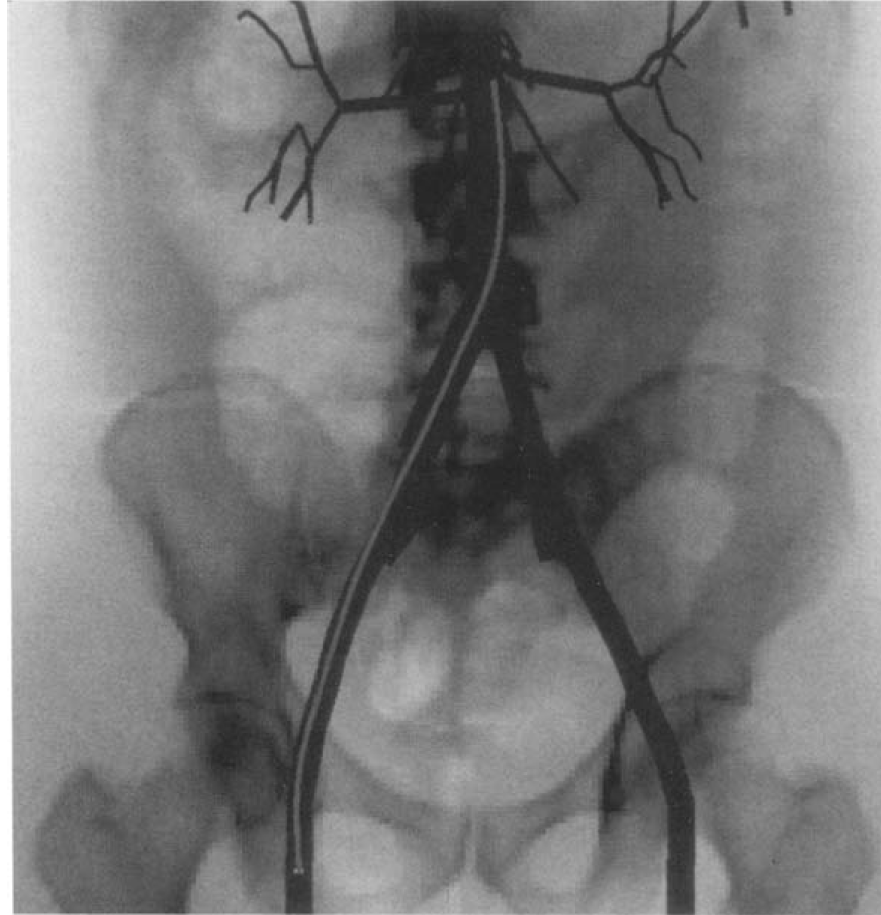
\includegraphics[scale=0.5]{Figures/DaVinci.png}
%\caption{新加坡国立大学和美国约翰·霍普金斯大学医学院共同研究的腹主动脉介入仿真训练系统daVinci\cite{Anderson1998daVinci}}
%\captionof{figure}[腹主动脉介入仿真训练系统daVinci]{新加坡国立大学和美国约翰·霍普金斯大学医学院共同研究的腹主动脉介入仿真训练系统daVinci\cite{Anderson1998daVinci}}
%\label{fig1-1}
%\end{figure}

几乎与此同时,开发daVinci的科研团队在前期工作的基础上,先后实现了用于心血管介入仿真训练的ICard系统(\textbf{\textit{I}}nterventional \textbf{\textit{Card}}iology Simulator) \cite{Wang1997ICard,Chui1998ICard,Wang1998ICard,Cai2004ICard,Cai2006ICard},以及用于脑血管介入仿真训练的NeuroCath系统(\textbf{\textit{Neuro}}radiology \textbf{\textit{Cath}}erization Simulator) \cite{Ma2000NeuroCath,Nowinski2000NeuroCath,Ma2001NeuroCath,Li2001NeuroCath,Nowinski2001NeuroCath,Anderson2001NeuroCath,Chui2002NeuroCath,Anderson2002NeuroCath,Ma2004NeuroCath,Volkau2005Vessel,Ma2005NeuroCath,Ma2006NeuroCath,Ma2006aNeuroCath,Ma2007NeuroCath}。%

ICard系统的应用目的是为医学院学生和医生提供一个能够方便地温习心血管介入疗法的平台,同时还希望兼顾评价使用者的技能水平。
该系统的软件部分提供了血管的立体模型和X光效果的显示 \cite{Wang1998ICard,Wang1998aICard}。
血管的影像数据主要来源于VHP。
对于手术涉及的主干血管,限于当时计算机的处理能力,研究团队使用Adobe Systems公司的Photoshop从每张横切影像中将感兴趣的区域中的血管影像的围线标出,然后再计算血管的中心线,最后结合中心线上各点的坐标和相应的半径,得到血管的模型 \cite{Wang1998ICard}。%
对于病灶涉及的冠状动脉,由于尸体的血管内并没有血液流动以及因此产生的压力,因此这部分较细的血管就会因为其周围肌肉组织的挤压而导致严重变形,这也就造成VHP数据中,冠状动脉的数据几乎全部被破坏 \cite{Wang1998ICard}。%
为了解决这个问题,该团队的研究人员利用三次元量床(\textbf{\textit{C}}oordinate \textbf{\textit{M}}easuring \textbf{\textit{M}}achine,CMM)\cite{CMMweb}来扫描冠状动脉的钢质模型 \cite{KyotoModelweb},从而获得包括完整冠状动脉分支的仿真血管网络,再经过后期的细部处理,得到满足系统要求的冠状动脉血管模型 \cite{Wang1998ICard}。%
此外,ICard系统还提供了人体的脑血管模型 \cite{Serra1997Vessel,Poston1995Vessel},而脑部影像数据是一组核磁共振血管影像 \cite{Wang1998ICard}。
然后,他们通过配准将上述的心脑血管模型与VHP中的主干血管模型连接在VHP数据构建的解剖环境中来获得完整的血管模型 \cite{Wang1998ICard}。
至于导管的建模,该系统同样采用了有限元方法 \cite{Wang1998ICard}。
ICard提供了两种不同的交互方式:一种是计算机界面,另一种是物理装置界面 \cite{Wang1998ICard}。
前者通过点击图形界面上的按钮;后者则通过专门设计的物理装置(导管移动传感装置,\textbf{\textit{C}}atheter \textbf{\textit{M}}ovement \textbf{\textit{S}}ensor device, CMS) \cite{Lim1998ICard,Lim1997ICard}。%
ICard的软件系统所支持的功能包括X光影像显示、立体影像显示与横切面显示、生物医学信号模拟、球囊与支架的植入、以及诸如造影剂的注射等 \cite{Wang1998ICard}。

NeuroCath用于仿真球囊和支架的安置、动脉瘤弹簧圈栓塞术(Aneurysm Coiling)等脑血管介入手术。
它继承了前两个系统的许多成熟技术和特性,包括:基于有限元方法的导丝建模以及导丝与血管壁相互作用建模 \cite{Wang1996daVinci,Chui1996daVinci}、基于多模态影像的血管中心线提取 \cite{Wang1998ICard}、以及X光效果的显示\cite{Wang1998aICard,Wang1998ICard}等。%
在此基础上,该系统为使用者提供了尽可能丰富和接近真实的体验。如:造影剂注入后在血管内扩散现象、虚拟病人在虚拟手术过程中的生理表征等。
为获得NeuroCath系统所需的脑血管模型,Cai等人 \cite{Ye2002Vessel,Cai2003aVessel,Cai2003Vessel}采用了一种利用扫描和混合操作以生成血管段和分岔的结构性方法,该方法提高了血管分岔处的光滑度;Volkau等人 \cite{Volkau2005Vessel,Volkau2008Vessel}在此基础上提出了基于血管中心线的重建方法,该方法首先提高了血管中心线的光滑程度;其次抑制了在分割和骨架化过程中引入的噪声,从而提高了(重建血管时所依赖的)血管半径的精确度。%
NeuroCath的操作风格与ICard类似,也提供了可视界面交互和物理交互装置交互两种方式 \cite{Nowinski2001NeuroCath}。
其中,研究人员为NeuroCath专门设计了物理交互装置 --- TiC(\textbf{\textit{T}}actile and \textbf{\textit{i}}mage \textbf{\textit{C}}ontrol)\cite{Chui1999TiC} \cite{Ma1999TiC},它由触觉子系统和影像操作子系统等两个主要部分组成。%
前者可以使操作者能够操作导管和导丝进行与真实血管介入手术中类似的运动;后者则通过一台虚拟工作站来操作可视界面中提供的X光影像的视角。
此外,NeuroCath还能为使用者提供血管内的视角,该功能用于血管内窥镜导航的仿真 \cite{Nowinski2001NeuroCath}。
NeuroCath最初在约翰-霍普金斯大学医学院进行了验证,随后还获得了包括德国萨尔大学诊断介入神经放射学诊所、中国北京宣武医院、以及德国国立信息技术研究中心等医院和研究机构的验证许可,并收到了比较满意的反馈 \cite{Ma2007NeuroCath}。%

为了提高工作效率,科研团队还开发了若干CAD软件,它们分别用于导管等血管介入器械,如:CathWorks \cite{Cai1998CathWorks,Cai2000CathWorks}、DCSM \cite{Li2001DCSM}等;以及血管等人体器官的建模的CAD软件工具,如:VasWorks \cite{Cai2003Vessel}、Vascular Editor \cite{Ma2007NeuroCath}等。%

近几年,该团队仍有部分研究人员致力于心血管介入手术仿真的研究,重点是心脏建模 \cite{Chiang2011,Chiang2012}等。

位于美国麻省的三菱电气实验室(Mitsubishi Electric Research Laboratories,MERL) \cite{merlweb}和美国创新微创疗法中心(Center for Innovative Minimally Invasive Therapy,CIMIT) \cite{cimitweb}联合发起了ICTS项目 \cite{Dawson2000ICTS,Cotin2000ICTS,Shaffer1999ICTS}。%
ICTS的全称是“Interventional Cardiology Training System”(介入心脏病学训练系统),该系统旨在为学习者提供训练平台,并为引入新的医学器材和手术方法提供展示平台 \cite{Cotin2000ICTS}。%
ICTS实现了X光效果的解剖环境、建立了导管的物理模型和血液流动模型、并制作了触觉接口装置 \cite{Cotin2000ICTS}。%
此外,该系统还实现了一种手术学习机制“Virtual Rounds” \cite{Shaffer1999ICTS},该学习机制复现了心血管介入手术的基本步骤,为使用者的训练评估提供了基础。
文献 \cite{Dawson2000ICTS}中提到,ICTS系统当时正准备在欧洲投入其首次训练试验。

然而,当时的ICTS仅仅处于样机验证阶段,根据与比利时Guidant公司的合同,该项目后来被移交至英国Virtual Presence公司以完成系统的研发,并最终由瑞典Mentce公司 \cite{menticeweb}将其商业化 \cite{GuidantMenticeNewsWeb,coles2011surveyCRaIVE},这就是该公司的VIST系列产品。%
目前,VIST系列的两种仿真平台已经能够仿真的血管介入技术有:冠状动脉造影、心脏节律管理、跨室间隔穿刺、肾动脉介入、髂内动脉介入、膝关节以下血管介入、主动脉内窥修复、颈动脉介入、脑血管介入、子宫动脉栓塞术等 \cite{menticeweb}。%
其中已经获得医学验证的技术有:颈动脉介入手术的仿真训练 \cite{Dayal2004VIST,Hsu2004VIST,Nicholson2006VIST,Patel2006VIST,Cates2007VIST,VanHerzeele2009VIST},肾动脉介入术 \cite{Aggarwal2006,Glaiberman2008VIST},髂内动脉介入术 \cite{Chaer2006VIST,Berry2007VIST,VanHerzeele2008VIST},冠状动脉介入术 \cite{Gallagher2006VIST}等。%

CIMIT的Sim小组 \cite{medicalsimweb}和法国INRIA的Shacra团队 \cite{shacraweb}联合开发的EVE项目 \cite{Wu2005EVE}是一种用于仿真脑血管介入手术的系统。
它提供了适用于复杂血管系统内部的具有实时的碰撞检测和碰撞响应性能的导管有限元模型 \cite{dequidt2007EVE,Duriez2006EVE,Lenoir2006EVE,Lenoir2005EVE,Cotin2005EVE},具有X光显示效果的头颈部解剖模型 \cite{Wu2011EVE,Luboz2005EVE,Muniyandi2003EVE},以及血流动力学模型、虚拟造影剂、心脏搏动和呼吸 \cite{Wu2007EVE}等视觉效果。%
文献 \cite{Dequidt2008EVE}介绍了该团队进行动脉栓塞术中弹簧圈的仿真以及验证的情况。
操作装置方面,研究人员设计了专用的触觉接口装置ABEL和专用的径向跟踪装置Cain \cite{medicalsimweb}。

此外,Shacra团队在EVE等项目的工作基础上,开发并维护着一个专门用于医学仿真的工具库 --- SOFA(\textbf{\textit{S}}imulation \textbf{\textit{O}}pen \textbf{\textit{F}}ramework \textbf{\textit{A}}rchitecture) \cite{Allard2007SOFA}。%

意大利CRS4小组发起了ViVa项目(\textbf{\textit{Vi}}rtual \textbf{\textit{Va}}scular project) \cite{abdoulaev1998},该项目的研究目标是为现代血流动力学研究者和心脏内科医生提供一系列的工具,帮助他们分析和解释在研究和临床过程中遇到的不断增多的相关信息。%
这些工具包括:图像处理与分割、实时立体体数据可视化、立体几何重建、立体网格生成、以及血流仿真和可视化等。
在此基础上,Gobbetti等人 \cite{Gobbetti1998}研究并实现了用于仿真血管镜的系统。
该系统以从标准医学影像模态所获取的数据作为输入,将其当作可供交互的虚拟环境;系统支持立体直接体绘制的实时导航和动态内窥镜的控制,可交互的组织分类,以及为实现形态学特性测量而摘取可交互点等。
Zorcolo与Gobbetti等人 \cite{Zorcolo1999,Gobbetti2000,Zorcolo2000}开发了一种实验性的导管插入系统。
该系统支持头部跟踪的立体视感,该视感通过从不同视角观察体重建而产生,体重建则与直接的立体触觉交互相匹配,这属于增强现实系统的范畴。

英国的CRaIVE(\textbf{\textit{C}}ollaborators in \textbf{\textit{R}}adiological \textbf{\textit{I}}nterventional \textbf{\textit{V}}irtual \textbf{\textit{E}}nvironments) \cite{CRaIVEweb}进行了与介入手术的仿真训练相关的研究。%
他们的研究主要集中于血管介入手术中血管系统的分割与重建 \cite{Luboz2008aCRaIVE},血管和导管及其相互作用的建模和验证\cite{Luboz2010CRaIVE,Luboz2009aCRaIVE,Luboz2008CRaIVE},Seldinger穿刺术的仿真\cite{luboz2009CRaIVE,John2008CRaIVE},以及穿刺术之前的腹股沟触诊的仿真\cite{Coles2011CRaIVE,Coles2009CRaIVE}。%
此外,文献 \cite{Coles2010CRaIVE}还对若干应用于穿刺仿真中的触觉反馈装置的性能进行了测试和比较。

法国巴黎第十二大学计算机工程与自动化实验室进行了基于虚拟现实技术的腹主动脉介入手术仿真系统的研究 \cite{Ghembaza2004Paris12U}。
系统中,腹主动脉和导管的物理模型采用基于位移的有限元方法来建立;为了实现连续的碰撞响应,研究人员采用了基于Cubic Spline的参数估计方法。

由荷兰列文胡克癌症研究所和乌德勒支大学图像科学研究所发起的MIVIS项目(\textbf{\textit{M}}inimally-\textbf{\textit{I}}nvasive \textbf{\textit{V}}ascular \textbf{\textit{I}}ntervention \textbf{\textit{S}}imulation) \cite{alderliesten2002NKI,Konings2003NKI,alderliesten2004NKI,Bosman2005NKI,alderliesten2007NKI,alderliesten2007aNKI}主要进行了腹主动脉导管介入的仿真,对导管在血管内的运动仿真是该项目的研究重点。%
血管的几何建模采用了Fuzzy Connectedness算法 \cite{Udupa1996NKI,alderliesten2002NKI,alderliesten2004NKI};而其物理建模则利用胡克定律来模拟血管壁的组织特性 \cite{alderliesten2002NKI,alderliesten2004NKI};导管模型的物理特性则建立在准静态力学(quasi-static mechanics)的基础上 \cite{alderliesten2002NKI,alderliesten2004NKI};并在此基础上进行了实物对比验证 \cite{alderliesten2002NKI,alderliesten2004NKI}。%
Konings等人 \cite{Konings2003NKI}提出了一种用于导管在血管内运动仿真的半解析算法,并进行了导管在平面弯道内运动仿真性能的验证分析。
Bosman等人 \cite{Bosman2005NKI}研究了利用一种进化算法以替代面向特定问题的一阶解析估计算法,从而解决仿真过程中的优化问题的优劣,并证明采用前者更有利于系统性能的优化。
Alderliesten等人 \cite{alderliesten2007NKI}又在此基础上进一步拓展了算法性能对比的研究,并证明采用共轭梯度算法或者进化算法能够在仅产生轻度误差的前提下,显著地减少计算时间。
文献 \cite{alderliesten2007aNKI}中报告了该项目中的导丝模型已经能够仿真导丝与血管壁之间的摩擦。

德国曼海姆大学、海德堡大学与德国维尔茨堡大学医院联合研究的CathI(\textbf{\textit{Cath}}eter \textbf{\textit{I}}nstruction System)用于血管介入尤其是经皮腔内冠状动脉成形术(\textbf{\textit{P}}ercutaneous \textbf{\textit{T}}ransluminal \textbf{\textit{C}}oronary \textbf{\textit{A}}ngioplasty,PTCA)的仿真 \cite{rebholz2004cathi,Hoefer2002CathI}。%
该系统提供了一系列的功能设施用于实现尽可能真实的血管介入手术仿真训练 \cite{rebholz2004cathi},包括:个人档案、不同型号的血管介入器械(导管、导丝、球囊和支架等)、控制C型臂的脚踏板、控制射线开关和造影剂剂量的设定、限制照射时间和介入手术总时间的设定以及人体生理指标的设定等。%
该系统的数据来自真实病例的术中X光造影,影像中能够观察到真实病例所具有的典型特征;而所选取的影像包含了一个心动周期的关键帧,因而能够提供准确的心脏搏动,这样可以为受训者提供最真实的视觉效果。
血管被抽象为刚体且横截面为圆 \cite{Hoefer2002CathI}。%
导管则被抽象为一列刚性的圆柱体,当导管与血管壁发生交互时,由这个几何模型确定其与血管壁的接触点,在此基础上计算应该发生的弯曲等形变,但未考虑导管与血管壁之间的摩擦 \cite{rebholz2004cathi}。%
在操作装置上,系统采用了导管室所使用的原始机构,最大限度地模仿真实的导管术操作工具;而测量导丝进给的功能实现上,则通过反射自附着在导丝上的玻璃纤维的光线的变化来测量导丝的运动,这种方法克服了传统机械方式所具有的摩擦和滑动等不足 \cite{Hoefer2002CathI}。%
此外,系统提供的个人档案功能能够记录受训者在仿真训练过程中的一些必要的信息,并且能够导出为Excel文件,但并未实现自动的评价功能 \cite{rebholz2004cathi}。

德国达姆施塔特科技大学和德国维尔茨堡大学医院进行了基于计算机仿真的冠状动脉造影中针对病例的导管最优选择方面的研究 \cite{Rahman2012Darmstadt,Rahman2011bDarmstadt,Rahman2011aDarmstadt,Flehmann2011Darmstadt}。%
工作的第一步是计算病例影像中主动脉的几何参数,一种新的分割后的融合方法被用于主动脉的几何模型的获取 \cite{Flehmann2011Darmstadt}。
在此基础上,文献 \cite{Rahman2011bDarmstadt,Rahman2011aDarmstadt}分别介绍了基于计算机仿真的左右两侧冠状动脉造影中针对病例的导管最优选择方法。
根据这两篇文献的结论,医师应能够更通过这些方法获得相应侧的冠状动脉介入时所需导管的最佳选择方案。
文献 \cite{Rahman2012Darmstadt}介绍了导管模型的建模方法,各种型号的导管的物理特性通过FEM方法进行建模,其具体工作使用了SOFA \cite{Allard2007SOFA}。

意大利莱切大学创新工程部的研究人员进行了心血管介入支架置入术仿真的研究 \cite{aloisio2006HERMES,aloisio2006aHERMES,aloisio2005HERMES,aloisio2004HERMES}。
其中的部分成果借鉴了由意大利CETMA集团发起的HERMES项目(\textbf{\textit{HE}}matology \textbf{\textit{R}}esearch virtual \textbf{\textit{ME}}dical \textbf{\textit{S}}ystem,用于血液学研究的虚拟医学系统) \cite{aloisio2005HERMES}。%
为了获得血管的准确形变,该系统采用有限元方法建立血管系统的模型 \cite{aloisio2004HERMES}。
系统的操作装置能够再现支架置入过程中,手术工具发生的形变 \cite{aloisio2005HERMES}。
不同于其它仿真系统的是,本系统还能够支持病例模型数据的网络检索和获取功能 \cite{aloisio2006aHERMES,aloisio2006HERMES}。
受训者可以利用这个功能,从支持相关数据共享的医疗机构获取需要的病例影像数据,这为病例数据的获取提供了极大便利,使受训者能够方便地接触到更丰富的病例。

瑞士洛桑联邦理工学院机器人系统实验室设计并实现了一种用于仿真脑血管介入手术的系统 \cite{Wang2007EPFL,Ilic2005EPFL,Moix2005EPFL,Ilic2005aEPFL,Ilic2005bEPFL}。
该系统的研究工作提出了一种基于物理特性的线形模型,以及一种快速碰撞检测策略 \cite{Wang2007EPFL}。
前者所体现的仿真物理特性模拟了导丝的弹性特征,后者可以提供连续的碰撞检测,这与中心线方法相比,能够揭露出血管壁表面的更多细节。
同样地,该系统也提供了X光显示效果的解剖环境。
此外,该实验室还设计并实现了用于脑血管介入手术仿真的4自由度触觉接口装置 \cite{Ilic2005EPFL,Moix2005EPFL,Ilic2005aEPFL}。
通过实验测量了血管介入手术中,血管因球囊膨胀过程中的弹性模量 \cite{Ilic2005bEPFL}。
根据文献 \cite{Wang2007EPFL},接下来的工作将是计算机仿真部分与触觉接口装置的整合。

日本名古屋大学的研究人员进行了用于分布式血管内遥操作手术的虚拟环境研究 \cite{Arai1994Nagoya,Arai1995Nagoya,Arai1996Nagoya}。
该虚拟环境主要为远离手术现场的医生提供直观的视觉和触觉。为此,该虚拟环境提供了三维显示功能和专门设计的操作机构。
显示功能中的血管和导管的建模都比较简化:导管模型以常数曲率弯曲、血管模型则被抽象为不同半径的圆柱体 \cite{Arai1994Nagoya,Arai1995Nagoya}。
该分布式遥操作手术系统用于脑血管介入手术,研究人员在东京市(早稻田大学)与名古屋市(名古屋大学)之间(距离350km)进行了实验。
整个过程中的数据通过异步传输模式的光纤传输 \cite{Arai1996Nagoya}。

日本名古屋大学微纳米系统工程系以及藤田保健卫生大学和安城厚生病院的研究人员进行了脑血管介入手术仿真的研究 \cite{Ikeda2004Nagoya,Ikeda2005Nagoya,Ikeda2005aNagoya,Ikeda2006Nagoya,Ikeda2007Nagoya}。%
与其他研究项目的思路不同,该项目的研究人员仍然坚持实物仿真训练,利用硅胶等材料、通过精密的加工工艺以人体头部CTA和MRA影像为依据,制作高精确度(解析度达到亚毫米级别)的人体脑血管的物理模型,为脑血管介入手术的训练提供操作场景 \cite{Ikeda2005Nagoya}。%
这种物理模型能够再现血管的物理特性,以及导管与其内壁发生的摩擦。

日本理化学研究所等科研机构开展了用于血管介入手术仿真的研究 \cite{takashima2009RIKEN,takashima2007RIKEN}。
导丝被抽象为若干段粘弹性弹簧(viscoelastic spring),其近端由于受限于导丝模型,故被抽象为刚性管道,而血管则被抽象为横截面为圆的弹性圆柱体 \cite{takashima2009RIKEN}。
血管的几何模型通过“分割血管-提取中心线-根据半径重建血管”的方式获得 \cite{takashima2009RIKEN}。
为了获得准确的、对导丝与血管壁之间相互作用的仿真效果,文献 \cite{takashima2007RIKEN}采取了实物试验与计算仿真相互比较的方法对这一场景下的摩擦和接触进行了实验和数值分析,从而得出仿真系统中准确的血管模型参数的重要性。%

日本香川大学工学部的郭书祥等人研究并实现了用于脑血管介入手术仿真的系统 \cite{Gao2012aGUO,Gao2012bGUO,Gao2012cGUO}。
该系统由为使用者提供视觉感受的虚拟现实软件和为使用者提供触觉感受的导管操作装置组成 \cite{Gao2012aGUO}。
在脑血管模型的获取过程中,研究人员通过若干开源工具,对血管影像进行阈值处理,手动记录血管的中心线坐标,使用一种被称为“四邻域法”的方法寻找血管的边缘像素点,在此基础上重建血管的几何模型 \cite{Gao2012bGUO}。%
导管模型的建立则采用了有限元的方法 \cite{Gao2012cGUO}。

美国HT Medical公司开发的CathSim系统用于仿真外周静脉内导管术 \cite{ursino1999cathsim},以及护理技术中的静脉穿刺 \cite{Barker1999CathSim}。

美国乔治·华盛顿大学研究了用于下腔静脉滤器置入的虚拟训练系统 \cite{Hahn1998GWU},该仿真系统提供下腔静脉滤器置入术的教学和测试。
为了获得X光的视觉效果,研究人员采用了一种“伪体绘制”的渲染方法 \cite{Park1996GWU},该方法能够生成影像数据的$360^\circ$的视觉效果,并且支持虚拟场景中摄像头沿虚拟人体的径向移动。
造影剂则被建模成粒子系统,该粒子系统由导管的尖端触发,系统则在不同的时刻进行记录其向心脏一侧运动过程中的位置 \cite{Hahn1998GWU}。
此外,该系统还能够模拟导管与血管壁之间的摩擦 \cite{Hahn1998GWU}。

加拿大的CAE公司 \cite{caeweb}开发了一种用于心血管介入的仿真训练系统CathLabVR。
该系统能够进行冠状动脉经皮介入、外周动脉经皮介入、以及心脏外科手术等的仿真训练。
以色列的Simbionix公司 \cite{simbionixweb}研发了一种用于血管介入的仿真训练系统Angio Mentor。
该系统能够进行介入式心脏治疗、介入式放射学诊断、血管手术、心脏手术、电生理学、介入式脑血管治疗、以及胸腔外科手术等的仿真训练。
文献 \cite{hislop2009Simbionix,Lee2012Simbionix}报告了该系统在实际使用情况。
文献 \cite{Petri2013Comparison}对主要的产品级别的仿真系统进行了临床验证。

美国的Medical Simulation公司开发了SimSuite \cite{simsuiteweb}系列血管介入手术仿真系统。
该系列中的Compass系统是一种便携式的仿真系统,这种系统为医师提供了随时进行进行基本流程的训练的条件。
该系列中的Infinity系统是一种能够运行在iPad等平板电脑上的仿真应用。
该系列中的Simantha系统是SimSuite的重量级系统,它能够支持心血管介入、脑血管介入、以及外周动脉介入等疗法的虚拟仿真。此外,该系统还支持用户建立自定义的训练课程。
文献 \cite{Dawson2007SimSuite}介绍了该系统的临床验证效果。

\subsection{国内研究现状}
\label{sec1-4-2}

近年来,随着我国社会经济的不断发展,国民生活水平也有了长足的提高,人们一方面享受到了较好的物质条件带来的多方面的益处,一方面也由于缺乏端正的健康生活意识而出现了各种由于膳食结构不合理、体力消耗水平过低而引起的疾病,其中以冠心病等心脑血管疾病为代表的人体循环系统疾病的发病率和致死率呈逐年上升趋势,这一趋势已引起了医学界和公共卫生部门的高度重视。
正是这样,国内高校和科研院所近年开展与临床手术应用相关的生物工程项目不断增多。
然而,由于我国在相关方面的科研基础与发达国家存在差距,再加上我们在科研成果转化为实际应用方面的滞后,目前,国内虚拟手术训练的研究仍处于初级阶段。

香港中文大学的计算机科学与工程系开展了血管介入手术仿真的研究 \cite{guo2007CUHK,Chui2010CUHK,Li2011CUHK,Li2012CUHK},并成为2009年该校举行50周年校庆时的重大成果之一 \cite{cuhkweb}。%
该系统的血管和导管的集合模型的建立,利用了中心线提取、图重建、曲线拟合、以及曲线帧技术;为了给形变模型赋予非线性的生物力学特性,采用了基于物理处理单元(Physics Processing Unit,PPU)的增量式Voigt模型 \cite{guo2007CUHK}。%
该系统通过一种非牛顿流的光滑粒子流体动力学(Smoothed Particle Hydrodynamics,SPH)形式来模拟血液在血管内的流变;通过流体结构相互作用的一种纯拉格朗日粒子形式来模拟血液与血管的相互作用,其中,血管壁结构被抽象为虚拟粒子;并在此基础上,模拟了血栓形成与消溶的过程 \cite{Chui2010CUHK}。%
导管与血管之间相互作用的模拟则基于最小总势能的原理,其中的势能是导管弯曲时的弹性势能、血管壁变形时的势能,以及外力所做功的总和;导管形变的模拟则利用了有限元的方法 \cite{Li2011CUHK}。%
此后,研究人员还研究了一种快速稳定的多网格求解器,以保证仿真的真实性和实时性 \cite{Li2012CUHK}。

中国科学院深圳先进技术研究院的马炘等人 \cite{Ma2010SIAT,Ma2010aSIAT}进行了脑血管介入手术仿真系统的研究。
该系统的脑血管建模,吴剑煌等人采用了面向三角网格的自适应细分模式 \cite{Ma2010bSIAT,Wu2006SIAT},所得血管模型的数据量得到了合理地精简,提高了血管模型在使用中的渲染速度和碰撞检测速度。%
导管等医疗器械的建模采用了有限元方法。导管被抽象为由许多节点相连的定长线段,对各个节点赋予物理属性,这样节点与节点就成了机构学上的铰接结构,当受到外力时,节点处可以自由旋转 \cite{Ma2010SIAT}。%
对导管与血管壁的相互作用的仿真,该系统的碰撞检测分为初步检测、精确检测、和确定碰撞位置等三个步骤 \cite{Ma2010SIAT}。
该系统还实现了触力反馈,并设计和实现触觉反馈装置 \cite{Ma2010SIAT}。

国防科技大学的熊岳山等人对虚拟心脏介入手术的相关方面进行了研究,如:
几何模型构建技术 \cite{han2005master}、
血流模拟和特效场景 \cite{ren2005master,Ren2006NUDT}、
弹簧-振子模型 \cite{wang2006master,Wang2008NUDT}、
医疗器械的三维建模 \cite{zhu2007master}
以及碰撞检测技术 \cite{kang2007master}等,
最近,该系统已经初步实现,文献 \cite{Tan2012NUDT}报告了该工作的最新进展。
其中,心脏模型的构建利用了Delaunay三角化方法,血管建模则采用了NURBS曲面;
通过组合弹簧振子联动模型的方法仿真了心脏搏动 \cite{Wang2008NUDT};
采用风腔结构 \cite{Ren2006NUDT}模拟冠状动脉和主动脉,提高了血流仿真效果。
此外,该系统还实现了虚拟造影剂、X光显示效果、以及导管等柔性器械的建模 \cite{Tan2012NUDT}。

其中与本课题研究方向有一定关系的有:
天津大学的冯鹰 \cite{li2005master}等人于2005年设计并实现了用于腹腔镜手术的虚拟训练系统;
该校的王树新等人 \cite{zeng2006master}于2006年研究了面向显微外科手术的虚拟血管缝合仿真系统。
上海交通大学的顾力栩等人开展了虚拟手术系统中模拟手术场景的渲染和平台的创建工作 \cite{zheng2008master}以及血管内血流模拟方面的工作 \cite{huang2011virtual};
该校的谢叻等人则在虚拟手术的碰撞检测 \cite{wu2010virtual}和触力反馈 \cite{wu2011virtual}方面进行研究。
复旦大学进行了房间隔缺损介入封堵术的三维可视化模拟 \cite{Zhao2006Fudan}。
北京工业大学研究了心血管系统动脉粥样硬化病灶部位的血流动力学 \cite{Huang2003BJUT}。
%# -*- coding:utf-8 -*-
\section{本文布局}
\label{sec1-4}

本文所述工作的目的是:研究创建冠状动脉介入导管术过程中所涉及的人体解剖环境的虚拟模型的方法,为仿真系统的解剖环境创建功能的实现提供关键技术支持。
冠状动脉介入导管术过程所处的解剖环境包括冠状动脉与主动脉组成的血管网络、冠状动脉围绕的心脏、躯干等。
在本研究项目中,创建解剖环境就是利用图像处理、计算机图形学、生物力学、流体力学等学科的技术,以真实病例的CT血管造影数据为基础,重建解剖环境中各个器官的几何模型,进而模拟其外观和物理特性,最终为使用仿真系统的用户提供足够真实的视觉感受。

本文开篇介绍本研究项目的基本情况,以及与本研究项目有关的同行的研究进展;接下来的每章叙述一个导管术训练系统的关键技术环节;最后一章总结我们在研究工作中的成果,经验,与教训,并展望本项目未来的一些可能的发展动向。全文分为正文和附录等两部分。
正文共八章:第一章是全文绪论,概括介绍本项目的研究动机、研究背景、以及本文的主要内容,详细描述与本文所述工作相关的典型样机和关键技术在国内外研究情况和发展历史;
第二章是医学背景介绍,比较详细地记述了与本文所述工作相关的医学知识,包括介入心脏病学和医学影像技术等内容;
第三章是血管模型的可视化,介绍了为从CTA中获得血管系统所对应的像素信息所进行的主要工作以及工作成果,详细描述本环节工作所用到的关键技术内容,以及在此基础上获得血管系统的可视化模型所进行的主要工作以及工作成果,深入描述了本环节工作所用到的关键技术内容;
第四章是心脏模型的提取与可视化,介绍了基于CTA的心脏模型的分割与可视化工作和工作成果,描述了本环节工作所用到的关键技术内容;
第五章是组织的物理特性建模,具体介绍了器官组织物理特性的分析与建模过程;
第六章是手术过程中特殊动态效果的实现,描述了为实现诸如虚拟造影剂、可视化模型的X光显示等可视效果而做的工作,展示了工作成果;
第七章是手术流程的状态机模型研究,主要介绍将冠状动脉导管术的流程进行计算机建模的一种方法;
第八章是总结与展望,客观、全面地总结全文内容,概括本研究项目所取得的工作成果,列出在此过程中表现出来的一些教训,最后对本研究工作的未来发展做了一些预测。
附录共两章,附录A给出了正文中的一些原理的数学推导;附录B记录了笔者在本项目的研究过程中对软件工程的一些思考。
文末附有参考文献和本人在学期间发表文章的清单等。

本文所述工作是“经皮介入冠脉导管术仿真系统的设计与研究”的一部分,工作任务涉及血管系统和心脏等解剖结构的场景生成和仿真。
关于该仿真系统中的手术工具的物理建模与仿真,请参考组内同事米韶华的博士学位论文《XXX》以及相关的已发表科技文章。

本文所述工作获得了国家自然科学基金(61225017)和北京市优秀博士学位论文指导教师科技项目(YB20108000103)资助。
在此,笔者谨向国家自然科学基金委员会和北京市教育委员会表示由衷的感谢!  
%# -*- coding:utf-8 -*-
\chapter{系统概观}
\label{chap2}

%# -*- coding:utf-8 -*-
本章叙述内容:
\begin{itemize}
  \item 介入心脏病学
  \item 医学影像技术
\end{itemize}
%# -*- coding:utf-8 -*-
\section{介入心脏病学}
\label{sec2-1}

本节叙述内容:
\begin{itemize}
  \item 
  \item
  \item
\end{itemize}

血管介入疗法根据其作用的血管系统的不同可以分为:神经介入疗法;心脏介入疗法;外周血管介
入疗法等。神经介入疗法专注于人的脑血管的导管介入治疗,用于治疗中风等脑血管疾病;心脏介
入疗法专注于人的心血管的导管介入治疗,用于治疗冠心病等心血管疾病;外周血管介入疗法专注
于人体外周血管系统的介入治疗\cite{coles2011surveyCRaIVE}。
%# -*- coding:utf-8 -*-
\section{医学影像技术}
\label{sec2-2}

本节叙述内容:
\begin{itemize}
  \item X光与CT \cite{Orosco2013Review}
  \item MRI
  \item Ultrasound
\end{itemize}

%# -*- coding:utf-8 -*-
\chapter{基于CTA的主动脉的分割与可视化}
\label{chap3} \fontsize{12pt}{12pt}\selectfont

%# -*- coding:utf-8 -*-
\section{Introduction}
\label{sec3_0}

Cardiovascular diseases are one of the main causes of death in the modern world.
%Recent years, they have also become one of the most killing illnesses in mainland China \cite{moh2004annual,moh2007annual,moh2010annual}.
The common causes of CVDs are the obstructive alterations occurred in the cardiovascular system.
Defects in one's life style are proved to play significant roles in the forming of the diseases, ranging from cigarette smoking and lack of physical exercises to the unhealthy diet and overweight and obesity \cite{Go2013}.

PTCA is an important medical skill for the cardiologists and has been proved to be a standard procedure to cure many kinds of CVDs, due to the small incision, short operation time, and quick recovery.
%This technique is an important medical skill for the cardiologists.
For the nature of this technique, the surgeons in this specialty have to gain solid understanding of vascular anatomy, choose the tools (catheters and guidewires) appropriately, and overcome the difficulties of the eye-hand coordination and the lack of sense of tactile \cite{Li2012CUHK}.
The other side of the coin is that during this complex procedure, the surgeons and the catheterization lab staff have to stand beside the bed to manipulate the tools, wearing bulky lead shielding aprons to protect themselves from the fluoroscope.
The harsh working conditions poses inevitable occupational hazards to the surgery practitioners \cite{Klein2009}.
Long hours of standing can raise orthopedic injuries and spinal disc diseases; therefore it leads to reduced working performance \cite{Goldstein2004}.
Moreover, the long-term ionizing radiation may induce an increased risk of brain malignancies \cite{Roguin2012}.
% So it requires sufficient learning and training from novice to master.
% Additionally, there are some precious opportunities for the trainee---to watch the real operations performed by the seniors in the catheterization labs.

The invention of medical robots has changed surgical practice as tasks are simplified and procedure time is reduced, while the clinicians are protected from the prolonged radiation exposure and the hand trembling is isolated.
Medical robots have been widely used in various clinical specialties, examples are orthopedics, neurosurgery, etc.
Nowadays, robot-assisted systems are also being developed and validated in catheterization labs in the hope of applying this innovative technology to save more lives.
A number of successful cases are Niobe magnetic navigation system from Stereotaxi Inc. \cite{NIOBEWeb}, the SenseiRobotic Catheter System from Hansen Medical \cite{HansenWeb}, Remote Navigation System (RNS) from Navicath \cite{Beyar2006RNS}, and CorPath 200 from the alliance of Phillips and Corindus Inc \cite{Smilowitz2012}.

To master the robot-assisted procedure, one must learn how to use the robot in sufficient time before his/her first real surgery.
It means that the training needs certain plants or objects to operate on -- something that provides enough details relating to the anatomy structures.
Traditionally, hospitals and medical institutions used to train their residents in this specialty by performing the procedures on donated or unclaimed cadavers, living animals (especially pigs), and sorts of physical mannequins and their variations made of plastics or some other non-biological materials \cite{Lunderquist1995,Mori1998}.
However, there are still many problems, for instance, cadavers are in scarcity and are dead for a time so that there is no blood flow in their vessels; the anatomy of living animals share only a few similarities to human's and performing biological and medical experiments on them often raise arguments from the society.
What's worse, while both preserving cadavers and raising animals cost too high, they can be used for training purposes just once.
Physical models seem to solve most of the problems: they offer fluid flow in the vessels and mimic anatomic structures, and are relatively affordable and can be reused.
However, they do need to be maintained and they have limited service periods.

Compared to the aforementioned methods, computer-aided surgical simulation demonstrates its advantages:
\begin{itemize}
\item no radiation risks;
\item less loss of details of the related anatomic structures;
\item free from restrictions of the schedule;
\item no extra costs for further use.
\end{itemize}
Computer-aided surgical simulation emerged and had quickly become an innovative and safe method in the training of many different medical procedures.
Numbers of robotic surgical simulators for the training of the famous da Vinci surgical robot are designed.
For example, dV-Trainer from Mimic \cite{Liss2012}, RoSS from Simulated Surgical Systems \cite{Kesavadas2011}, ProMIS from CAE \cite{Jonsson2011} and SEP robot simulator from SimSurgery \cite{Meijden2010}, etc.
Many research institutions have also devoted in the field of interventional cardiology and various prototypes for vessel intervention were born in 1990s, such as Dawson-Kaufman simulator \cite{Dawson1996DK}, ICard \cite{Wang1997ICard}, ICTS \cite{Cotin2000ICTS}, etc.
ICTS was turned into a commercial product by Mentice \cite{MenticeWeb} after the final work completed.
Some other commercial products were also provided, for instance, CathLabVR manufactured by CAE \cite{CAEWeb}, ANGIO Mentor invented by Simbionix \cite{SimbionixWeb}, etc.
However, to our best knowledge, most of them are designed to train their users how to do PTCA in traditional manners.

%Vessel models are the most important virtual scenarios required in this kind of training, thus making vessel segmentation an important step.

In this paper, the aim is to provide the three dimensional aorta model based on real patient's medical data for the robotic training system, which is designed for the intravascular surgical robot developed in our lab \cite{Ji2011CASIA}.
As the first task in constructing the vessel model, segmentation of abdominal aorta from the CTA series is challenging, because the aorta and the bones often adhere together.
This makes the aorta hard to segment cleanly.
To address this problem, a robust and semi-automatic approach is developed.
This approach makes the geodesic active contours method \cite{Caselles1997} as its core function which performs the segmentation on CTA series and produces the 3-D surface model of the abdominal aorta.
The 3-D model provides one of the important parts of the anatomic scenario for the simulation of PTCA procedures.
The experimental results showed that this approach is capable of segmenting the aorta in CTA series.
%The goal of this work is to extract the lumen of the abdominal aorta from CTA series and reconstruct the 3-D surface model of the aorta based on the segmented information.
%The methods and experiences should be easily ported to our further work related to the reconstruction of other organs in the anatomic scenario.

The rest of this paper is organized as follows.
Section II describes of the structure and techniques in the segmentation.
% Then the rest of this section is divided into four parts:
% First, the work flow and the main methods employed to produce the feature images are described.
% Second, the methods for the generation of the initial level set are introduced.
% Third, the core armed with geodesic active contours method is described in mathematical details.
% In the end, the method used for visualizing the segmented vasculature is given.
Section III details the experiments and presents the results.
The final section concludes the whole work. %and predicts the future work.
%# -*- coding:utf-8 -*-
\section{引言}
\label{sec3-1}

正如本文开篇所述,心血管疾病是一类对人类健康构成严重危害的疾病。
为了对这类疾病进行精确的诊断和治疗,研究人员已经成功研究了许多成像技术(见第\ref{sec2-2}节)。
血管系统本身特有的复杂的空间结构和多变的形态,决定了血管影像的大信息量、复杂特征。
于是,对血管影像的分割就成了一个通往血管模型的精确可视化的关键步骤。
在此基础上,医生才能对病情进行准确的诊断和治疗。
目前,尽管研究人员开展了大量关于血管分割的研究工作——有的已取得不俗成果,有的仍在进行;但是,血管分割仍然是一项极富挑战性的任务\cite{Lesage2009Review}。
没有一种分割方法能够独自解决当前所有影像模态获取的影像的分割问题。
分割完成后就要对分割所得信息进行图形处理,从而显示血管系统的几何外形。
我们采用行进立方体(Marching Cubes)方法\cite{Lorensen1987MC}将血管外表面所对应的像素值决定的空间曲面提取出来。
为了后续工作的需要,我们采用XXX方法计算血管模型的中心线;
利用XXX方法精简构成血管模型的多边形的数量;
利用XXX方法对多边形数量精简后的血管模型进行多边形三角化;
利用XXX方法对三角化后的血管模型进行几何外观上的平滑处理。

本章的叙述将按照研究工作的顺序依次展开。
首先,介绍基于CTA的血管系统的分割,描述工作中先后采用的两种不同分割技术的原理与实现,以及各自在算法层面的性能,并简要说明这两种技术各自的优势和劣势。
其次,介绍血管模型的可视化,描述工作中采用的主要技术方法的原理与实现。
再次,展示血管建模的实验结果。
最后,给出这部分工作的阶段性结论。
%# -*- coding:utf-8 -*-
\section{基于CTA的血管系统的分割}
\label{sec3_2}

血管分割是一项难度较大的任务,其难度在于\cite{Lesage2009Review}:
一是影像采集过程中对信息造成的损害,如:对比度、解析度、噪声等;
二是血管系统本身的复杂结构,空间分布复杂、粗细和弯曲程度不一;
三是血管内部的支架、钙化物、血管瘤、管腔狭窄等能对血管系统的外观和几何结构产生影响;
四是血管系统深植于人体复杂的解剖环境当中,彼邻其他器官。
此外,由于血管影像的上述特点,使得血管影像的数据量很大、血管的图像特征很复杂,这都给图像分割算法的运算性能提出了更高的要求。

血管分割技术被广泛应用于脑、心、肺、肝、肾、以及肢体外周等部位的血管系统的分析与诊断。
获取血管影像的医学影像模态包括磁共振和CT等。
根据分割结果的不同,血管分割可分为血管腔分割、血管外壁分割、以及血管内血栓分割\cite{Lesage2009Review}。
由于血管成像时,对比剂的增强效果只能使血管内腔在影像中得以保留,故血管腔分割相对容易;而血管外壁和管内血栓的分割则相对较难。
在本文中,我们仅讨论与经皮冠状动脉导管介入术相关的血管系统的分割,影像模态为CT,影像中包含了病例人体的躯干,扫描时对血管系统进行了增强。
因为我们仅仿真血管内部的情况,所以只需进行血管腔的分割。

用于血管分割的方法多种多样,根据其基本的提取策略可以将这些方法分为区域生长法、活动围线法、以及基于中心线的方法。

\subsection{区域生长方法}

区域生长法是一类基于区域的图像分割方法,它的运行从最初给定的“种子区域”开始,根据使用者预先定义的“生长准则”把符合要求的像素或者子区域合并成为较大区域。
其中,“种子区域”通常是一个或多个像素(二维情形)或者体素(三维情形)。
“生长准则”则是根据处理任务而制定的,其主要限定特征是像素(或者体素)的灰度值或颜色\cite{Gonzalez2004Matlab}。
区域生长法所得结果就是使用者“感兴趣的图像区域”,使用这种方法进行分割的目的就在于此,这一目的能否达成,依赖于“种子”的选取和“生长准则”的制定。
表征区域生长法区别的主要特征有:“生长准则”、确定邻接像素的邻域连接类型、以及寻找邻接像素的策略\cite{Ibanez2005ITKGuide}。
区域生长法主要用于图像分割、以及图像的预处理等场合。

理想情况下,区域生长法的操作始于种子点的选取。
然后,我们将这些种子点分为$n$组(对应于分割目标中的$n$个物体),$A_1, A_2, \ldots, A_n$。
各分组中的种子点的个数可以为$1$,即该组中仅含有一个种子点,分组总数也可以为$1$,即分割目标只有一个。
接着,区域生长法在此基础上会求出一个对作用图像的曲面细分(Tessellation),这个细分将原图像划分为若干区域。
这些区域都具有这样的性质,即一个区域中,每个连接到的分量都与某一组种子点$A_i$相连。
受此约束,所选的区域都尽可能是“齐次的”\cite{Adams1994SRG}。

算法的每一步都在演进,借以向上述的种子点的集合中的其中一个添加一个像素。
现在,我们考虑该算法运行$m$步后,集合$A_i$的状态。
如果我们用$T$来表示所有与上述区域邻接而尚未被重新分配的像素的状态,那么
\begin{equation}
\label{eq3-1}
T = \left\{x\notin\bigcup_{i=1}^{n}A_i|N(x)\cap\bigcup_{i=1}^{n}A_i\neq\varnothing\right\}
\end{equation}
其中,$N(x)$是像素$x$邻接区域中像素所组成的集合。
下面,我们假定所讨论的算法作用于平面图像上,一个像素与其周围的像素的邻接形式是$8$-邻域。
若$\forall x\in T$,
则以$i(x)\in \left\{1, 2, \ldots, n\right\}$为上述某种子点集合$A$的下标,该集合满足$N(x)\cap\bigcup_{i=1}^{n}A_i\neq\varnothing$。
以$\delta(x)$表示$x$与其邻接区域的不同程度。
该$\delta(x)$可表示为
\begin{equation}
\label{eq3-2}
\delta(x)=\left|g(x)-\underset{y\in A_{i(x)}}{mean}[g(y)]\right|
\end{equation}
其中,$g(x)$是图像在像素$x$处的灰度值。
若$N(x)$与两个或更多的$A_i$集合相交,那么我们就将$i(x)$作为$i$的值,使得$N(x)$与$A_i$相交,且$\delta(x)$最小。
或者,在同样情况下,我们可能需要将$x$归为一个边界像素,并将之添加到集合$B$中,该集合包含了那些已经被发现的边界像素。
标定这些边界像素对满足显示需要或者下文提到的半交互修正流程都很有用。
我们取$z\in T$,使得
\begin{equation}
\label{eq3-3}
\delta(z)=\min\limits_{x\in T}{\left\{\delta(x)\right\}}
\end{equation}
并将$z$添加到$A_i(z)$中。

至此,算法就完成了第$m+1$步。
整个算法将依照上面介绍的过程重复运行,直到所有的像素都被恰当地分配为止。
此过程开始于每个种子点的集合$A_i$互不相交。
式\ref{eq3-2}和式\ref{eq3-3}所给出的定义保证在考虑连接性的约束的前提下,最终的分割结果由尽可能“齐次的”区域组成。

在区域生长法的程序设计中,我们采用了串列顺序列表(Sequential Sorted List, SSL),也就是计算机算法理论中的链表(Linked List)。
在区域生长法的情景下,SSL其实就是分割过程中,原始图像中的像素被读入内存后的地址,这些像素地址根据某种属性进行排列。
当在区域生长法的每一步开始时,我们从SSL的起始处取要考虑的下一个新像素。
当一个像素要被添加至SSL的时候,我们必须根据其自身具有的排序属性来选定这个像素在SSL中的位置。
在我们讨论的这种情况中,SSL根据$\delta$来收储集合$T$中的数据。

实现上述算法(边界标定的情形)的伪代码如下:
{\renewcommand{\baselinestretch}{1}{
\begin{algorithm}[htb]                    %算法的开始
\caption{\textsc{Seeded Region Growing}}  %算法的标题
\label{alg:SRG}                           %给算法一个标签,这样方便在文中对算法的引用
\begin{algorithmic}[1]   %不知[1]是干嘛的?
%\REQUIRE ~~\\            %算法的输入参数:Initialization
%  Set $J=0$; $S_0  = \left\{ \phi  \right\}$; $R(S_0 ) = 0$; $\Omega=\{1,2,\ldots,K\}$;
\ENSURE ~~\\             %算法的迭代:Iteration
%Ensemble of classifiers on the current batch,  $E_n$;
%\WHILE    {$J<M$}
%\STATE $J\leftarrow J+1$;
%    \FORALL {$k\in \Omega$}
%    \STATE  $R_{temp}=0$;  $\Delta R_{J,k} = R(S_{J-1}\cup \{k\})-R(S_{J-1})$;
%         \IF  {$\Delta R_{J,k}>0$}
%            \IF{$R(S_{J-1}\cup \{k\})\geq R_{temp}$}
%            \STATE $R_{temp}\leftarrow R(S_{J-1}\cup \{k\})$; $s_J\leftarrow k$;
%            \ENDIF
%         \ELSE
%            \IF{$1/(1-\Delta R_{J,k}/c_k )<rand(1)$}
%            \STATE $\Omega= \Omega-\{k\}$;
%            \ENDIF
%         \ENDIF
%    \ENDFOR
%\IF {$R_{temp}>0$}
%\STATE $S_J\leftarrow S_{J-1}\cup \{s_J\}$;
%\ELSE
%\STATE $J\leftarrow J-1$; Break;
%\ENDIF
%\ENDWHILE              %算法的返回值

\STATE Label seed points according their initial grouping.
\STATE Put neighbors of seed points (the initial T \ref{eq3-1}) in the SSL.
\WHILE {$SSL\neq \varnothing$}
    \STATE Remove first point $y$ from SSL.
    \STATE Test the neighbors of this point:
    \IF {all neighbors of $y$ which are already labeled (other than with the boundary label) have the same label}
        \STATE Set $y$ to this label.
        \STATE Update running mean of corresponding region.
        \STATE Add neighbors of $y$ which are neither already set nor already in the SSL to the SSL according to their value of $\delta$.
    \ELSE
        \STATE Flag $y$ with boundary label.
    \ENDIF
\ENDWHILE
%\LASTCON ~~\\          %OUTPUT
%  selected user set $S_J$ and weighted sum rate $R(S_J)$;

\end{algorithmic}
\end{algorithm}
}}

区域生长法充分图像的局部空间信息,它能有效地克服利用其他方法进行分割时,所得结果中有可能存在的图像空间不连续的问题。
然而,作为一种低层的图像分割方法,区域生长法也存在着一些不足。
首先,区域生长法在克服了前述问题的同时,容易造成过度分割(使分割结果中包含了一些使用者“并不感兴趣的区域”);
其次,区域生长法依赖人工交互以获得使处理得以进行的“种子”——这是由其基本特征所决定;
最后,区域生长法对图像中的噪声比较敏感,因此在引入这类方法之前,必需对被处理图像进行降噪处理。
除此之外,由于区域生长法属于串行算法,当欲分割目标较大时,处理速度就会明显变慢。
因此,在诊断场合中,此类方法一般用于对肿瘤和伤疤等目标进行分割。
%# -*- coding:utf-8 -*-
\section{Methodologies}
\label{sec3_3}

In this section the overall processing pipeline is discussed and the techniques used for the lumen segmentation of the abdominal aorta from CTA are detailed.
% The original data adopted in our work is a series of CTA images with the dimension of $512\times512\times90$.
% The series are acquired from the trunk of the patient with CVDs.

The overall design of the pipeline is illustrated in Fig. \ref{fig:DataFlow}.
The format and data type of original images are firstly converted.
Then the conditioned data is fed into two branches to produce the two inputs required by the main segmentation module.
One branch performs several preprocessing work on the images to produce the feature images. %, including smoothing, gradient magnitude computation, and intensity mapping.
And the other branch computes the initial level sets of the images. %, including a mini level set branch which requires numbers of seeds.
After the branches end the computation, their production are fed into the main segmentation module, where the actual interface evolution takes place.
In the final phase, the output level sets are extracted and then visualized by using a surface rendering technique.
%The parameters and seeds are provided manually and tuned repeatedly during the processing.
\begin{figure}[t]
\centering
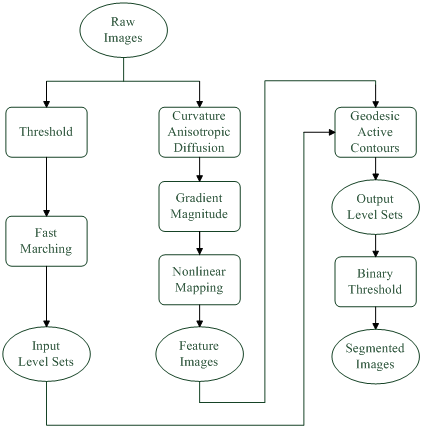
\includegraphics[width=3.2in]{Figures/chap03/DataFlow.png}
\caption{An overview of the segmentation pipeline.}
\label{fig:DataFlow}
\end{figure}

\subsection{Preprocessing}

Before the main processing begins, several necessary pretreatment on the original images should be done.
By considering the requirements of the methods chosen for this job, the preprocessing should include the production of feature images, and the generation of input level sets.
The feature images provide the main level set method with the ``maps" about where to stop, while the input level sets give the main functioning module the initial contours from where the actual interface evolution begins.

\subsubsection{Production of Feature Images}

%The branch of feature image production is depicted in Fig. \ref{fig:DataFlow}.
Image smoothing is a necessary job due to the original series acquired from the medical modality are often mixed with some noisy pixels.
What to take care of is that the original edges of the target (i.e., aorta) should be preserved as completely as possible while removing the noises.
Bear this in mind, a level-set curvature method with variable conductance \cite{Whitaker2001} is chosen for the job.
This method is good at enhancing and preserving edges, and is robust to the edge contrast.
It can be described as the following \emph{modified curvature diffusion equation} (MCDE):
\begin{equation}
\label{eqn:MCDE}
I_t = |\nabla I| \nabla \cdot c(|\nabla I|) \frac{\nabla I}{|\nabla I|},
\end{equation}
where $I = I(x, y, 0)$ represents the input image, $I_t(\cdot) = I(x, y, t)$ represents the output image generated over time $t$, and $c$ is the conductance function given by
$c(|\nabla I|) = k^2/(k^2 + |\nabla I|^2)$ with $k$ a parameter which determines the contrast of boundaries that will have significant effects on the smoothing.

After that, the computation of gradient magnitude is performed on the resulting series to detect the edge of target.
Since the feature images to be produced are required by the downstream geodesic active contours module, the most important step in this series of tasks is the computation of the magnitude of gradient pixel-wisely for the images:
\begin{equation}
\label{eqn:Gaussian}
I_{grad} = \exp(-|(\nabla \ast G) \cdot I_t|),
\end{equation}
where $I_{grad}$ is magnitude of the gradient at some point in the image, and $\nabla \ast G$ means the first order derivative of a Gaussian operator.

The computed edge images are mapped through a nonlinear relation (usually represented in the form of an S-shaped function) in order to get the feature images:
\begin{equation}
\label{eqn:Sigmoid}
I_{\sigma} = (I_{max} - I_{min}) \cdot \frac{1}{1 + \exp\left(-\frac{I_{grad} - n}{m}\right)} + I_{min},
\end{equation}
where $I_{\sigma}$ denotes the intensity values of the output image, $I_{max}$ and $I_{min}$ represent the maximum and minimum of the output intensity values, respectively; $m$ is a constant that controls the width of the input intensity range, and $n$ is a constant that gives an intensity around which the range is centered.
The mapping results may vary due to different choices of the parameters for the individual modules in the pipeline.

\subsubsection{Semi-Automatic Generation of Input Level Sets}

%The initial level set generation branch is parallel to the above one, which is responsible for the computation of the values required by the main evolution as its input level sets (see Fig. \ref{fig:DataFlow}).
% This branch is a mini level set that takes numbers of seeding points (or seeds) before the computation begins.
The first pass is a thresholding procedure that will strip out most of the irrelevant details of the images.
After the thresholding is done, the fast marching algorithm \cite{Sethian1999} could focus its evolution on the target with the appropriately selected seeding points.
For the curve $\mathcal{C}$ evolving over time $t$
\begin{equation}
\label{eqn:Curves}
\mathcal{C}(t) = \{(x,y) | T(x,y) = t\},
\end{equation}
where $(x,y)$ represents some point in the image, and $T(x,y)$ is the time of arrival.
The algorithm solves the following Eikonal equation (which is in fact a stationary Hamilton-Jacobi equation)
\begin{equation}
1 = | \nabla T | F,
\end{equation}
where $F$ denotes the velocity in the normal direction at some point $(x,y)$.
$\mathcal{C}$ propagates inwards when $F < 0$; it propagates outwards when $F > 0$.
The results of this computation are the time-crossing map in which contains of a series of curve interfaces at different time of evolution.

\subsection{Geodesic Active Contours Evolution}

%The module that actually working towards the segmentation is illustrated in Fig. \ref{fig:DataFlow}.
At this point, the geodesic active contours module has its two inputs available: the feature images and the initial level sets.
The feature images provide the maps for the interface evolution initialized by the input level sets.
The classical ``snakes" or active contour models for boundary detection were proposed by Kass et al. \cite{Kass1988}.
The idea is to evolve a contour $\mathcal{C}$ such that the edge of the object can be detected.
This evolution is achieved by minimizing an energy functional whose (local) minimum can be found at the edge of the object.
% This energy functional of the contour $\mathcal{C}_0$ in the classical snakes approach is given by (the denotation is adopted from \cite{Caselles1997})
% \setlength{\arraycolsep}{0.0em}
% \begin{eqnarray}
% \label{eqn:Snakes}
% E(\mathcal{C})&{}={}&\alpha \int_0^1 |\mathcal{C}'(q)|^2 dq + \beta \int_0^1 |\mathcal{C}''(q)|^2 dq \nonumber \\
                  % &&{-}\:\lambda \int_0^1 |\nabla I ( \mathcal{C}(q) ) | dq,
% \end{eqnarray}
\setlength{\arraycolsep}{5pt}
% where $\mathcal{C}(q)$ denotes the parametrized planar curve $\mathcal{C}(q):[0,1]\rightarrow \mathrm{R}^2$, $I:[0,a]\times [0,b]\rightarrow \mathrm{R}^{+}$ represents an image on which the edge detection task is carried out, and $\alpha$, $\beta$, and $\lambda$ are all real positive constants.
% The first two components control the smoothness of the curves to be detected, and the last one propagates the curve outwards (or inwards) until it ``touches" boundaries of the objects in the given image.
% The classical problem is to find the curve $\mathcal{C}$ that minimizes the energy functional $E$, for the given constants $\alpha$, $\beta$, and $\lambda$.
However, the curve in this approach cannot deal with the change of its topology so that detecting more than one object in the image is impossible without additional procedures \cite{Caselles1997}.
Caselles \textit{et al.} \cite{Caselles1997} improved the classical ``snakes" by proposing the geodesic active contours method, which allows to detect both the internal and external boundaries of several objects simultaneously.
This method incorporates the concepts of geodesic computation and level set evolution.
The proposed model is a particular case of the classical model:
\begin{equation}
\label{eqn:ParticularSnakes}
E(\mathcal{C}) = \alpha \int_0^1 | \mathcal{C}'(q) |^2 dq - \lambda \int_0^1 | \nabla I_{s} ( \mathcal{C}(q) ) |dq,
\end{equation}
where $\mathcal{C}(\cdot)$ denotes the parametrized planar curve $\mathcal{C}(q):[0,1]\rightarrow \mathrm{R}^2$, $I_{s}:[0,a]\times [0,b]\rightarrow \mathrm{R}^{+}$ represents an image on which the edge detection task is carried out.

To minimize the functional defined by (\ref{eqn:ParticularSnakes}), the curve at the points of maxima $|\nabla I_{s}|$ must be located.
During this process, certain level of smoothness of the curve also needs to be kept.
In (\ref{eqn:ParticularSnakes}), $|\nabla I_{s}|$ can be substituted by $-g(|\nabla I_{s}|)$, where $g(\cdot): [0, \infty) \rightarrow \mathrm{R}^{+}$ is a monotonically decreasing function. %such that $\lim_{x \to \infty} g(x) = 0}$.
Hence, a general energy functional is obtained
\begin{equation}
\label{eqn:GeneralEnergy}
E(\mathcal{C}) = \alpha \int_0^1 | \mathcal{C}'(q) |^2 dq + \lambda \int_0^1 g( | \nabla I_{s} ( \mathcal{C}(q) ) | )^2 dq.
\end{equation}
The aim of the evolution is trying to obtain
\begin{equation}
\label{eqn:MinModel}
\min \int_0^1 g(|\nabla I_{s} ( \mathcal{C} (q) )|) |\mathcal{C}' (q)| dq.
\end{equation}
% Thus the problem has been shifted from the minimization of (\ref{eqn:ParticularSnakes}) to the geodesic computation.
In (\ref{eqn:GeneralEnergy}), $g(\cdot)$ is equivalent to the speed of the evolution of the curve.
And it is also dependent upon the geometry of the image content.
For the ideal edges of the objects to be detected, the choice of parameter $g(\cdot)$ is independent of their geodesic computation.
So the minimum given in (\ref{eqn:MinModel}) can be rewritten as:
\begin{equation}
\label{eqn:MinModel2}
\min \int_0^1 g(I_{\sigma}) |\mathcal{C}' (q)| dq.
\end{equation}
To obtain the minimum given in (\ref{eqn:MinModel2}), the following Euler-Lagrange associated with this model needs to be calculated
\begin{equation}
\label{eqn:EvolutionModel}
\frac{\partial \mathcal{C}(t)}{\partial t} = g(I_{\sigma}) \kappa \mathcal{N} - (\nabla g(I_{\sigma}) \cdot \mathcal{N}) \mathcal{N},
\end{equation}
where $\kappa$ is the curvature of $\mathcal{C}(t)$, $\mathcal{N}$ is the unit inward normal vector. %, and the right-hand side of the equation is the computation of Euler-Lagrange.
This equation presents the way $\mathcal{C}$ evolving towards the boundaries of the objects to be detected.
The initial curve is marked as $\mathcal{C}(0) = \mathcal{C}_0$, which evolves to a (local) minimum of (\ref{eqn:MinModel2}).

According to (\ref{eqn:EvolutionModel}), this evolution will stop when $\frac{\partial \mathcal{C}(t)}{\partial t} = 0$, meaning that the boundaries of the objects are detected.
Suppose that the curve $\mathcal{C}$ is a level-set of a function $u(\cdot):[0,a] \times [0,b] \rightarrow \mathrm{R}$.
Regarding (\ref{eqn:MinModel2}) and (\ref{eqn:EvolutionModel}), the former geodesic calculation is transformed to finding the steady state solution of the following equation:
\begin{equation}
\label{eqn:LevelSetModel}
\begin{split}
\frac{\partial u}{\partial t} & = |\nabla u| \textrm{div} \left(g(I_{\sigma}) \frac{\nabla u}{|\nabla u|}\right) \\
                              %& = g(I_{\sigma}) |\nabla u| \textrm{div} \left(\frac{\nabla u}{|\nabla u|}\right) + \nabla g(I_{\sigma}) \cdot \nabla u \\
                              & = g(I_{\sigma}) |\nabla u| \kappa + \nabla g(I_{\sigma}) \cdot \nabla u,
\end{split}
\end{equation}
where $\kappa = \textrm{div}\left(\frac{\nabla u}{|\nabla u|}\right)$.
The right-hand side of this equation is the Euler-Lagrange of (\ref{eqn:MinModel2}).
% Here in this equation, $u$ is the embedding function mentioned above that deforms according to $u_t = \beta |\nabla u|$, where $\beta$ is a function computed on the level sets.
% From the perspective of image segmentation, a positive real constant $c$ is introduced in order to detect the boundaries of a non-convex object using a convex initial curve
% \begin{equation}
% \label{eqn:ImprovedLevelSetModel}
% \begin{split}
% \frac{\partial u}{\partial t} & = g(I) |\nabla u| \textrm{div} \left(\frac{\nabla u}{|\nabla u|}\right) + c g(I) |\nabla u| \\
                              % & = g(I) ( \kappa + c ) |\nabla u|.
% \end{split}
% \end{equation}

In order to increase the ``attractive force" to the contour towards the edges and allow the detection of non-convex objects, the term $cg(I_{\sigma})|\nabla u|$ is added to (\ref{eqn:LevelSetModel}):
\begin{equation}
\label{eqn:Geodesic1}
\frac{\partial u}{\partial t} = |\nabla u| \textrm{div} \left(g(I_{\sigma}) \frac{\nabla u}{|\nabla u|}\right) + c g(I_{\sigma}) |\nabla u|,
\end{equation}
where $c$ is a constant and $c \in \mathrm{R}^+$.
Regarding (\ref{eqn:LevelSetModel}), the above equation can be rewritten as
\begin{equation}
\label{eqn:Geodesic2}
\frac{\partial u}{\partial t} = g( I_{\sigma} )( c + \kappa ) |\nabla u| + \nabla u \cdot \nabla g(I_{\sigma}).
\end{equation}
% which means that the level sets move according to
The above equation can be transformed to the following equation
\begin{equation}
\label{eqn:Geodesic3}
\frac{\partial \mathcal{C}}{\partial t} = g(I_{\sigma}) ( c + \kappa ) \mathcal{N} - ( \nabla g(I_{\sigma}) \cdot \mathcal{N} ) \mathcal{N}.
\end{equation}
The solution to this object detection problem is equivalent to the zero level-set of the steady state ($u_t = 0$) of (\ref{eqn:Geodesic1}).
%Comparing (\ref{eqn:EvolutionModel}) and (\ref{eqn:Geodesic3}), one can find an added term $c g(I_{\sigma}) \mathcal{N}$, which is corresponding to the
% For the ideal edges of the objects to be detected, the choice of parameter $g$ is independent of their geodesic computation.
% It is a very simple edge detector which is given by the following equation
% \begin{equation}
% \label{eqn:EdgeDetector}
% g = \frac{1}{1+\|\nabla \hat{I}\|^p},
% \end{equation}
% where $\hat{I}$ denotes a Gaussian-smoothed image of the original $I$ and $p$ is the exponential of $\hat{I}$.
% What we are interested in is the time when the curve interface corresponding to the edges of the target.
% After the evolution stopped, a binary thresholder is provoked to take a ``snapshot" of this interface.
% This resulting level set should be the edges of the objects to be detected.

\subsection{Surface Extraction}

To visualize the surface model, the surface information should be firstly extracted by the marching cubes method \cite{Lorensen1987MC}.
As the initial step of surface extraction, arrays of cubes are created from the input with each cube consisting of eight pixels (four from one slice and the other four from the next slice).
Then the index for each cube is calculated by comparing the eight intensity values to the specified isovalue corresponding to the surfaces of the objects.
By referring to the triangulated cases with the indexes, the intersection patterns of the objects and the cubes can be roughly determined.
Then the precise edge intersections are computed using linear interpolation with the intensity values at each vertex of the cubes.
After that, the unit normals to the surface at each vertex of these cubes are computed via central differences.
The resulting triangles are then sent to the graphics systems and displayed by standard rendering techniques.
% The isovalue representing the edge of the segmented target is selected.
% Then the 3-D model of the target can be reconstructed.
% That is the 3-D surface model of the lumen of the aorta.
%# -*- coding:utf-8 -*-
\section{Experiments and Results}

\subsection{Experimental Setup}
Many experiments were carried out using different parameters for the validation of the approach to segment the aorta from CTA.
In our case, the CTA series in DICOM format had been converted to the form of XML first.
Then the converted data was fed into the feature image production branch and input level sets generation branch.
The resulting data from the two branches were sent to geodesic active contours module in order to generate the final results.
Finally, the marching cubes method is used to visualize the segmented data.
The experiments were all run on a machine with Intel's 2.83GHz Core 2 Quad CPU and 4GB RAM.

The input series was obtained by a 128-slice Siemens SOMATOM Definition Flash CT with the slice thickness of 0.6mm.
And the series contains the patient's entire abdominal aorta.
For illustrative purposes, a typical slice was selected from the series.
To reduce the computation time, the region that contains the major branches of the abdominal vasculature in the selected image were cropped (see Fig. \ref{fig_roi}).
\begin{figure}[t]
\centering
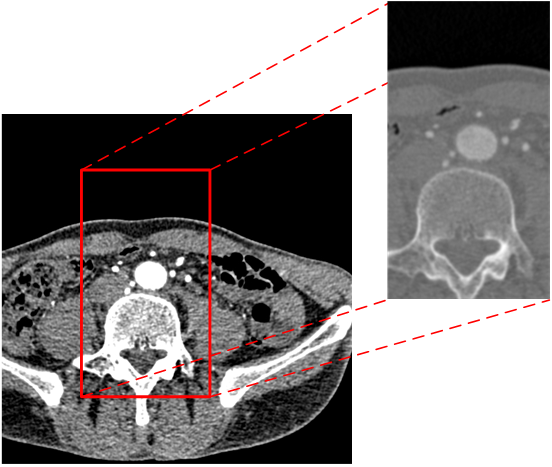
\includegraphics[width=2.5in]{Figures/chap03/ROI.png}
\caption{A typical ROI extraction of the original slice.}
\label{fig_roi}
\end{figure}
% Then the segmentation process was split into two branches first and then merged into the main evolution pipeline.
%This two-branching structure is built due to the two essential requirements of geodesic active contours module: the feature images and initial level sets.

\subsection{Feature Images}
In the feature image production branch, the following preprocessing tasks were performed sequentially:
\begin{enumerate}
\item removing noises without affecting the edges;
\item computing the gradient magnitude pixel-wisely;
\item mapping the intensity into the required feature.
\end{enumerate}
At the beginning, a level-set curvature method with variable conductance was utilized to perform the smoothing task.
It is an edge-preserving smoothing method that can remove the unnecessary noises from the images while preserving the nature of the boundaries of the objects.
The image was smoothed nicely and the boundaries of the aorta even the minor vessels (which means weaker edges) were preserved (see Fig. \ref{fig:Smoothing}).
Then the gradient magnitude module was introduced to fulfill the requirements of gradient computing.
It computes the magnitude of the gradient pixel-wisely for the image by performing the convolution with the first order derivatives of a Gaussian kernel defined by (\ref{eqn:Gaussian}).
%The only parameter of the kernel is its deviation $\sigma$ and we set it to 0.9.
The edges of the vessels, bones, and skins were extracted completely in the resulting image (see Fig. \ref{fig:Gradient}).
After computing the magnitude of the gradient, the non-linear intensity mapping was employed to generate the edge potential map.
The choices of the parameters in (\ref{eqn:Sigmoid}) heavily depends on extreme values of the pixel intensities in the gradient image.
In this case, to reverse the relationship between objects (in low intensities in the gradient map) and their edges (in high intensities in the gradient map), $m$ was set to be a negative value and $n$ to be a positive value which is larger than $|m|$.
The mapping produced the expected feature image with the proximities of the edges of the objects in zero intensity (see Fig. \ref{fig:Sigmoid}).
This made the evolution of the level sets driven by (\ref{eqn:Geodesic3}) propagated faster in the ``flat area" (with uniformly high intensities), whilst much slower (in a speed of about zero) in the ``ridge" (with rapid decreasing intensities).
\begin{figure*}[t]
\centering
%\subfloat[Smoothing with edge preserving (Conductance parameter = 0.9)]{\includegraphics[width=1.2in]{fig/dcm_smoothing.jpg}%
\subfloat[]{\includegraphics[width=1.2in]{Figures/chap03/dcm_smoothing.jpg}%
\label{fig:Smoothing}}
\hfil
%\subfloat[Computation of magnitude of gradient with Gaussian kernel ($\sigma = 0.9$)]{\includegraphics[width=1.2in]{fig/dcm_gradient.jpg}%
\subfloat[]{\includegraphics[width=1.2in]{Figures/chap03/dcm_gradient.jpg}%
\label{fig:Gradient}}
\hfil
%\subfloat[Nonlinear mapping using an S-shaped function ($m = -3$, $n = 20$)]{
\includegraphics[width=1.2in]{fig/dcm_sigmoid.jpg}%
\subfloat[]{
\includegraphics[width=1.2in]{Figures/chap03/dcm_sigmoid.jpg}%
\label{fig:Sigmoid}}
\caption{Producing the feature image in three steps: (a) smoothing with edge preserving ($\text{conductance parameter} = 0.9$); (b) computation of magnitude of gradient with Gaussian kernel ($\sigma = 0.9$); (c) nonlinear mapping using an S-shaped function ($m = -3$, $n = 20$).}
%\caption{Producing the feature image.}
\label{fig:PotentialImageGeneration}
\end{figure*}
\begin{figure*}[t]
\centering
%\subfloat[Thresholding]{\includegraphics[width=1.2in]{fig/dcm_threshold.jpg}%
\subfloat[]{\includegraphics[width=1.2in]{Figures/chap03/dcm_threshold.jpg}%
\label{fig:Threholding}}
\hfil
%\subfloat[Level set evolution using fast marching method]{
\includegraphics[width=1.2in]{fig/dcm_fastMarching.jpg}%
\subfloat[]{
\includegraphics[width=1.2in]{Figures/chap03/dcm_fastMarching.jpg}%
\label{fig:FastMarching}}
\hfil
%\subfloat[Edge detection using geodesic active contours]{
\includegraphics[width=1.2in]{fig/dcm_geodesic.jpg}%
\subfloat[]{
\includegraphics[width=1.2in]{Figures/chap03/dcm_geodesic.jpg}%
\label{fig:GeodesicActiveContours}}
\hfil
%\subfloat[Binary thresholding]{
\includegraphics[width=1.2in]{fig/dcm_out.jpg}%
\subfloat[]{
\includegraphics[width=1.2in]{Figures/chap03/dcm_out.jpg}%
\label{fig:BinaryThresholding}}
\caption{Level set evolution: (a) thresholding ($\text{lower threshold} = 300\text{HU}$, $\text{higher threshold} = 2000\text{HU}$); (b) initial level set evolution from one seeding point using fast marching method; (c) edge detection using geodesic active contours; (d) binary thresholding to inverse the pixel intensities (intensity of the light area: $255$, intensity of the dark area: $0$).}
\label{fig:LevelSetEvolution}
\end{figure*}

\subsection{Level Sets Evolution}
The initial level set generation branch works for the level sets that required by the geodesic active contours module.
In this process, the thresholding module was called first to trim off the irrelevant organs with lower intensities, such as lungs, liver, kidneys, bowels, stomach, etc. (see Fig. \ref{fig:Threholding}).
%In our case, we set the lower and upper threshold values at 300HU (HU is short for Hounsfield Unit) and 2000HU, respectively.
This can further reduce the hunger for memory and dramatically shorten the computation time.
When finished this, the fast marching module is provoked to generate the initial interfaces.
One seed located interior of the region representing the aorta was fed to this module in this two dimensional image.
% And these seeds evolved the interfaces surrounding themselves respectively towards each other (see Fig. \ref{fig:FastMarching}).
And the time of arrival $T(x,y)$ given in (\ref{eqn:Curves}) were computed (see Fig. \ref{fig:FastMarching}).
Considering the prolonged geometric nature of the aorta and the characteristics of the algorithm, multiple seeding points inside the space representing the aorta should be fed in the three dimension case to acquire better results and much shorter computation time.
% We set the stopping time for the fast marching filter in order to shorten the time for the generation of initial level sets.

% \subsection{Geodesic Evolution}
The geodesic active contours evolution began working when all the preceding computation finished.
The module took the feature image and the initial contours as its inputs.
The contours evolved by the drive defined by (\ref{eqn:Geodesic3}) with the feature image as their reference.
The segmentation module evolved the contours until the edges were met (see Fig. \ref{fig:GeodesicActiveContours}).
After that, a binary thresholding step was performed to fill the inner area of the final contours as the light zone while the outer area as the dark zone.
This result is illustrated in Fig. \ref{fig:BinaryThresholding}.
All the parameters chosen manually to make the drive suitable to evolve the contour to the expected results were reused in the three dimensional case.

\subsection{Surface Construction Based on Segmentation Results}
Finally, the resulting volume were processed using the marching cubes method \cite{Lorensen1987MC}.
The isovalue corresponding to the edge of the lumen of abdominal aorta was picked manually.
Here the higher threshold value of the binary thresholder was provided as the isovalue for the isosurface extraction.
This ensured that the rendered surface representing the surfaces of the lumen of the aorta.
The final visualization model is depicted in Fig. \ref{fig:VisualizationModel}.
%From this figure, we can see that the lumen of the aorta was extracted successfully using the approach described here.
\begin{figure}[t]
\centering
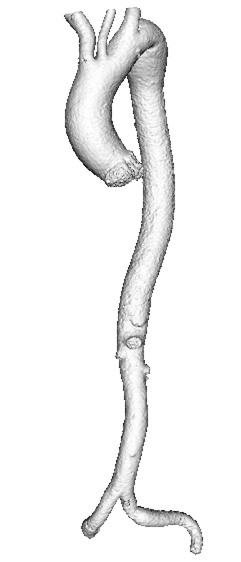
\includegraphics[width=1.1in]{Figures/chap03/model.png}
\caption{3-D surface model of the lumen of the aorta.}
\label{fig:VisualizationModel}
\end{figure}
%# -*- coding:utf-8 -*-
\section{Conclusions and Future Work}
%The conclusion goes here.

The three dimensional model of the aorta is one of the most important parts of the virtual scenarios of the robotic training systems which is built for the intravascular surgical robot.
In this paper, a robust and semi-automatic vessel segmentation approach based on geodesic active contours method has been proposed.
After reporting the design and considerations of the experiments, the results as well as the analysis were presented.
The lumen model of the aorta was then reconstructed by the marching cubes method using the segmented volumetric data.
The experimental results showed that the approach can successfully deal with the messy part due to the anatomic nature of the adherence of the aorta and the spine; and can accurately gain the vessel model.

% The pipeline in this paper was programmed mostly in C++.
%Some of the imaging filters were implemented based on the Insight Toolkit (ITK) \cite{Ibanez2005ITKGuide}.
The data format of the original CTA series were firstly converted.
Then the converted data was fed into the pipeline and was transferred into two branches: one for the production of featured images, and the other for the production of initial level sets.
The production served as the input of geodesic active contours module.
%Moreover, we also provide series of parameters for this module thus it can start the interface evolution.
The evolution stopped after a specified number of iterations and the binary threshold module was called to converse the pixel intensity.
Then the marching cubes implementation extracted the surfaces of the aorta in the segmented data before rendering.

As a future work, on the one hand the coronary arteries needs to be segmented and visualized in the volumetric data.
On the other hand, a series of post-processing work will be carried out in order to eliminate the artifacts and decimate the number of polygons that consisting the surface model.
The whole vasculature model will be available to the simulation tests of the models of the catheters/guidewires.
%Besides, the improvement of the visualization effect of the vessel model will also be an substantial work.
%During this process, a friendly software interface of the surgical simulator will be implemented.

%# -*- coding:utf-8 -*-
\chapter{基于CTA的冠状动脉的分割与可视化}
\label{chap4}

%# -*- coding:utf-8 -*-

The visualization of the coronary vasculature is of utmost importance in interventional cardiology.
Intravascular surgical robots assist the practitioners to perform the complex procedure while protecting them from the tremendous occupational hazards.
Robotic surgical simulation aims to provide support for the learners in both efficiency and convenience.
The blood vessels especially the coronary arteries with rich details are the key part of the anatomic scenario of the virtual training system.
The variations in diameters and directions make the segmentation of the coronary arteries a difficult work.
In this paper, a robust and semi-automatic approach for the segmentation of the coronary arteries is developed.
The approach is based on the multi-scale tubular enhancement and an improved geodesic active contours model.
The demonstrated approach firstly enhances the tubular objects by computing their ``vesselness".
Next the edge potential maps are calculated based on the enhanced information.
Meanwhile, the initial contours are generated by a modified fast marching method.
Then the actual wave fronts evolution extracts the details of the coronary arteries.
Finally the visualization model is organized based on the segmentation results by the marching cubes method.
This approach has been proved successful for the visualization of the coronary arteries based on the CTA information.

\section{Introduction}
\label{sec4_0}

Coronary artery diseases are one of the key causes of deaths in the modern world. % \cite{WHO2013}.
The fatty blood clot (or plaque) adhering to the inner wall of the tiny vessels can partly or completely block the supply of oxygen and other nutritious substances for the heart muscles.
The diseases may lead to serious or even fatal health problems, such as angina and heart attack \cite{OCallaghan2002}.
%The unhealthy living habits have been proved to be the main reasons that cause the fatal diseases \cite{Go2013}.
Percutaneous coronary intervention (PCI) is the standard clinical solution to the coronary heart diseases.
Comparing with the traditional paradigm of the thoracic surgery, this procedure causes much less incisions and trauma, shorter operation time and post-op observation.
Therefore, this skill lies at the core place in the toolkit of a cardiologist.
Regarding the minimally invasive feature of PCI, the clinicians need to master the insight of the complicated anatomic structures of the coronary arteries and the manipulation of the tools.
Moreover, they must conquer the difficulties of the coordination between eyes and hands during the procedure \cite{Li2012CUHK}.
However, risks arise.
Instances are orthopedic injuries turn out due to the prolonged standing and the heavy weight of the lead protection apron during the PCI procedure \cite{Goldstein2004}, and high incidence rate of brain tumors caused by the long-term ionizing radiation under the fluoroscope \cite{Roguin2012}.

To gain the mastery of this important and complex technique, one must endure sufficient and strict drills under the supervision of the mentor before his/her solo surgery.
Most of the medical institutions and hospitals used to train their residents/interns who aim to be a cardiologist mainly based on human cadavers and living animals \cite{Lunderquist1995}, as well as non-biological models \cite{Mori1998}.
Although these training methods successfully protect the trainees from the common occupational hazards, they also have their flaws:
there is no blood circulation in the human cadavers;
the animal's anatomic structures are different from the human's;
and the preservation of the cadavers and the raising of the animals cost a lot of money and all of them cannot be reused.
The physical models need to be routinely maintained and have limited lifetime, despite they can provide intuitive appearance of the human body.

Computer-aided surgical simulation demonstrates its unique characteristics, such as radiation-free, rich details of the procedure-related anatomy, schedule-free, and ease of maintain.
Numbers of simulation systems were developed in research institutions \cite{Dawson1996DK,Wang1997ICard,Cotin2000ICTS} and technological incorporations \cite{CAEWeb,MenticeWeb,SimbionixWeb}.

Intravascular surgical robots provide the cardiologists brand-new facilities to perform the PCI procedures \cite{NIOBEWeb,HansenWeb,Beyar2006RNS,Smilowitz2012}.
Since the manipulation of the robots are different from the traditional procedure, one needs to learn and practice in a series of lessons.
In this training process, new problems emerge.
First, training on the real robot systems is a huge waste of high-end medical resources.
Second, the robotic training shares the same problems with its traditional counterparts.
Robotic surgical simulation for the da Vinci system have proved successful in solving the problems \cite{Liss2012,Kesavadas2011}.

The aim of this work is to develop an approach to visualize the coronary arteries based on the computed tomography angiography (CTA).
The acquired model will be the critical part of the blood vessel model in the robotic intravascular surgical simulator designed for the robot-assist intravascular surgical system \cite{Ji2011EMBC}.
The segmentation of the coronary vasculature is a difficult and demanding work.
Due to their tiny scale and complex topology, the coronary arteries in CTA are often in relatively low intensities and the complicated details may get lost during the processing.
To address this problem, an approach based on the multi-scale tubular enhancement and an improved geodesic snakes is designed.
For a better segmentation, the vessels are enhanced at first.
The pixels are convolved with a Gaussian kernel to compute the Hessian matrix.
Then we take the eigenvalues of the matrix to calculate the ``vesselness" measure.
Next the speed images are generated by computing gradient and applying nonlinear intensity mapping to the enhanced images.
Simultaneously the initial level sets are generated by the improved fast marching algorithm.
After the above computation complete, the actual fronts propagation starts and the final segmentation results are conversed after the propagation ends.
Then the visualization model of the coronary arteries are extracted.
The experimental results demonstrate that the approach is capable of visualizing the coronary arteries in the CTA.

The rest of this paper is organized as follows.
Section II outlines the precessing work flow and details the techniques introduced in the segmentation tasks.
Section III describes the experiments and presents the results.
The final section concludes the whole work. 
%# -*- coding:utf-8 -*-
\section{Methodologies}
\label{sec4_1}

This section discusses the design of the segmentation pipeline and details the principles of the consisting modules.
Fig. \ref{fig:DataFlow} presents the block diagram of the processing pipeline in the bird's-eye view.
The data type of the pixels in the original images is firstly converted.
After the images are appropriately thresholded, the data needs to be enhanced appropriately, right before sending the data to the downstream modules.
The enhancement should highlight the ``tube-like" objects, which are the coronary arteries in this paper.
Next the intensities of the enhanced objects are tuned for the following processing.
Then two computations are performed simultaneously to generate the speed images and the initial contours for the CURVES system.
After that, the results are fed into the CURVES module, where the actual fronts propagation occurs.
The CURVES system can evolve the input contours with the reference of the speed images until the contours ``touches" the wall of the tiny vessels.
Finally the output contours are extracted and then visualized in the surface rendering way.
\begin{figure}[t]
\centering
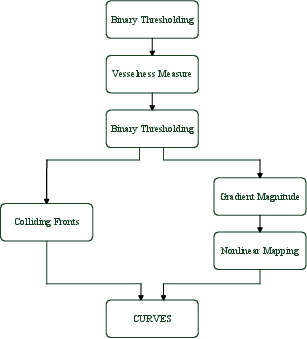
\includegraphics[height=3.2in,width=3.2in]{Figures/chap04/DataFlow.png}
\caption{Collaboration diagram of the segmentation pipeline.}
\label{fig:DataFlow}
\end{figure}

\subsection{Tubular Objects Enhancement}

The tubular enhancement is a sort of multi-scale line filtering, whose scheme can be summarized as the ``tube-like" objects in the image are highlighted whilst the rest are attenuated. %
To achieve this, the three dimensional multi-scale algorithm proposed by Sato \textit{et al.} \cite{Sato1998} is introduced.

To shape the filter response to certain width of lines and suppress the noisy effects, the pixels need to convolving with the second order derivatives of a Gaussian kernel.
This computation is an equivalent to the calculation of the Hessian matrix $\mathcal{H}$ of the three-dimensional image $I(\cdot)$:
\begin{gather}
\label{eqn:Hessian}
\mathcal{H} = \nabla^2 I =
\begin{bmatrix}
I_{xx} & I_{xy} & I_{xz} \\ I_{yx} & I_{yy} & I_{yz} \\ I_{zx} & I_{zy} & I_{zz}
\end{bmatrix},
\end{gather}
where $I_{xx} = \frac{\partial^2 I}{\partial^2 x}$, $I_{xy} = \frac{\partial^2 I}{\partial x \partial y}$, to name a few.
And all these partial second order derivatives are the convolutions with the second order derivatives of a Gaussian kernel $G(x; \sigma)$ with the standard deviation $\sigma$:
\begin{equation}
\label{GaussianConvolution}
I_{xx} = I \ast \frac{\partial^2 G}{\partial^2 x}.
\end{equation}
The eigenvalues of (\ref{eqn:Hessian}) are $\lambda_1$, $\lambda_2$, and $\lambda_3$ with their values in descending order.
Their associated eigenvectors are $e_1$, $e_2$, and $e_3$, respectively.

When $\lambda_1 \approx 0$ and $\lambda_2 \approx \lambda_3 \ll 0$, the line measure can be written as
\begin{equation}
\label{eqn:LineMeasure}
\lambda_{123} =
\begin{cases}
\left| \lambda_3 \right| \left( \frac{\lambda_2}{\lambda_3} \right)^{\gamma_{23}} \left( 1 + \frac{\lambda_1}{\left| \lambda_2 \right|} \right)^{\gamma_{12}}, & \lambda_1 \le 0 \\
\left| \lambda_3 \right| \left( \frac{\lambda_2}{\lambda_3} \right)^{\gamma_{23}} \left( 1 - \alpha \frac{\lambda_1}{\left| \lambda_2 \right|} \right)^{\gamma_{12}}, & \frac{\left| \lambda_2 \right|}{\alpha} > \lambda_1 > 0 \\
0, & \text{otherwise}.
\end{cases}
\end{equation}
In (\ref{eqn:LineMeasure}), the additional parameters $\gamma_{12}$, $\gamma_{23}$, and $\alpha$ are all positive constant, where $\gamma_{12} \in [0, \infty)$ is used to discriminate between the branching structures and the noises as well as pseudo-branches, $\gamma_{23} \in [0, \infty)$ regulates the sharpness, and $\alpha \in (0, 1.0]$ maintains the asymmetrical characteristics of the last terms of the function for all possible $\lambda_1$.

Additionally, different choices of the eigenvalues can equip the line filter with the abilities in detecting different shapes of the objects as shown in Table. \ref{tbl:Eigenvalues}. %

\subsection{Preprocessing for Level Set Evolution}

\subsubsection{Speed Images Calculation}

Level set algorithms evolves the contours in the gradient field with ``sharp" variations in intensity values from the inner or outer area to the boundaries.
The aim of the speed images is to provide this gradient field in the form of nicely shaped gradient images.
In the gradient images, the magnitude of the gradient at each pixel is calculated.
Next the gradient images $I_{\nabla}$ are transformed into the speed images $I_{\sigma}$ by applying the nonlinear relation:
\begin{equation}
\label{eqn:Sigmoid}
I_{\sigma} = (I_{max} - I_{min}) \cdot \frac{1}{1 + \exp\left(-\frac{I_{\nabla} - n}{m}\right)} + I_{min},
\end{equation}
where $I_{max}$ and $I_{min}$ are the two extreme values of the output intensity values, $m$ is a constant that controls the window width of the input intensity, and $n$ is a constant that defines the center of the window.
\begin{table}
\renewcommand{\arraystretch}{1.3}
\caption{Eigenvalue sets for detecting different shapes}
\label{tbl:Eigenvalues}
\centering
\begin{tabular}{l||c}
\hline
\bfseries Shape & \bfseries Eigenvalues \\
\hline\hline
Bright tubes   & $\lambda_1 \approx 0, \lambda_2 \approx \lambda_3 \ll 0$ \\
Dark tubes     & $\lambda_1 \approx 0, \lambda_2 \approx \lambda_3 \gg 0$ \\
Bright plates  & $\lambda_1 \approx \lambda_2 \approx 0, \lambda_3 \ll 0$ \\
Dark plates    & $\lambda_1 \approx \lambda_2 \approx 0, \lambda_3 \gg 0$ \\
Bright spheres & $\lambda_1 \approx \lambda_2 \approx \lambda_3 \ll 0$ \\
Dark spheres   & $\lambda_1 \approx \lambda_2 \approx \lambda_3 \gg 0$ \\
\hline
\end{tabular}
\end{table}

\subsubsection{Initial Contours Evolution Using Colliding Fronts}

The aim of the colliding fronts module is to evolve the contours for the CURVES system from the user-defined seeding points.
The colliding fronts method is implemented based on the principles of the fast marching algorithm \cite{Sethian1999}.
However, this method requires two seeds for each round of evolution such that the area between the seeds can be extracted.
The output of this module is the dot production of the gradient field of arrival times of the two wavefronts.
The level set initialization for the prolonged objects greatly benefit from this feature of the method.
On the other hand, the method also shortens the computation time.

\subsection{CURVES Evolution Model}

The CURVES method \cite{Lorigo2001} is chosen as the functioning segmentation method because of the complex nature of the coronary arteries.
It is highly effective in the segmentation of the complicated curvilinear structures in the volumetric medical images.
In addition, the criterion of CURVES method also takes the local smoothness of the boundaries to be detected (i.e., the inner wall of the coronary arteries) into account.

This method is a modification of the geodesic active contours method developed in Caselles \textit{et al.} \cite{Caselles1997}.
As the extensive research of the geodesic active contours, CURVES is a level set algorithm that models the tiny vessels as spatial curves with arbitrarily complicated topology \cite{Lorigo2001}. %
CURVES evolves the level sets to the boundaries of the targets based on the criterion of the minimization of the following energy functional
\begin{equation}
\label{eqn:CURVES}
\oint_0^1 g\left( \left| \nabla I \left( \mathcal{C} \left(  s \right) \right) \right| \right) \left| \mathcal{C}'\left( s \right) \right| ds,
\end{equation}
where $\mathcal{C}\left( s \right): [0,1] \rightarrow \mathrm{R}^3$ is a one-dimension curve, $I\left( \cdot \right): [0, a] \times [0, b] \times [0, c] \rightarrow [0, \infty)$ is an image on which the curve evolution takes place, and $g\left( \cdot \right): [0, \infty) \rightarrow \mathrm{R}^+$ is a monotonically decreasing function. %

The minimization of this functional can be achieved by searching for the gradient descent direction of the functional itself, which means the Euler-Lagrange equations associated with (\ref{eqn:CURVES}) needs to be computed. %
Thus the geodesic flow equation that controls the contour evolution in this process of minimization can be obtained as follows
\begin{equation}
\label{eqn:Evolution}
\frac{\partial \mathcal{C}}{\partial t} = k \mathcal{N} - \frac{g'}{g} \varPi \left( \mathcal{H} \frac{\nabla I}{ \left| \nabla I \right| } \right),
\end{equation}
where $\mathcal{H}$ is the Hessian matrix of the image $I$, $k$ is the Euclidean curvature, $\mathcal{N}$ is the unit normal vector, $\varPi(\cdot)$ is the projection operator projects the argument onto the normal space. %
The update equation can be obtained as
\begin{equation}
\label{eqn:Update}
\frac{\partial v}{\partial t} = \mathcal{F} \left( \nabla v(x, t), \nabla^2 v(x, t) \right) + \frac{g'}{g} \nabla v(x, t) \mathcal{H} \frac{\nabla I}{ \left| \nabla I \right| },
\end{equation}
where $v(\cdot): \mathrm{R}^3 \rightarrow [0, \infty)$ is the embedding function of the curve $\mathcal{C}$, $\mathcal{F} \left( \nabla v(x, t), \nabla^2 v(x, t) \right)$ is the smaller eigenvalue of the matrix $P_{\nabla v} \nabla^2 v P_{\nabla v}$. %
The matrix $P_q$ is defined as a projector which projects some vector onto the normal plane of vector $q \in \mathrm{R}^3$:
\begin{equation}
\label{eqn:ProjectionOperator}
P_q = I_0 - \frac{qq^T}{\left| q \right|^2},
\end{equation}
where $I_0$ denotes the identity matrix.

By incorporating the speed images $I_{\sigma}$ to the evolution equation (\ref{eqn:Evolution}), the evolution in our case can be obtained as
\begin{equation}
\label{eqn:Application}
\frac{\partial \mathcal{C}}{\partial t} = k \mathcal{N} - \frac{g'(I_{\sigma})}{g(I_{\sigma})} \varPi \left( \mathcal{H} \frac{\nabla I_{\sigma}}{ \left| \nabla I_{\sigma} \right| } \right).%
\end{equation}

\subsection{Surface Rendering}

The surface information is extracted for the visualization by the marching cubes method \cite{Lorensen1987MC}.
Cubes are created based on the input information and are organized into an array structure.
Each cube consists of eight pixels (each four pixels are from a slice).
The index of each cube is labeled by comparing the intensity values of every pixel to the isovalue of the surfaces.
Next the patterns of the intersection between objects and cubes are initially determined based on the triangulated cases.
Then the precise intersection are computed using linear interpolation with the intensity values at each vertex.
The unit normals to the surface are calculated via central differences for the vertices of the cubes.
Finally the generated triangles are ready for the surface rendering.
%# -*- coding:utf-8 -*-
\section{Experiments and Results}
\label{sec4_2}

\subsection{Medical Data and Experimental Setup}

The original chest CTA series was acquired by a 128-slice Siemens SOMATOM Definition Flash CT.
The slice thickness was $0.6 \text{mm}$ and the in-slice resolution was $0.4 \times 0.4 \text{mm}^2$.
Since the work was all on the coronary arteries, the volume contained the whole heart (i.e., ROI, which is the abbreviation of \textit{region of interest}) was cropped from the original data as shown in Fig. \ref{fig:Original}. %

Numbers of experiments were conducted with different sets of parameters to segment the coronary arteries from CTA for the testament of the approach in this paper.
In our case, the original CTA series in DICOM format had been converted to the form of XML first; and the data type of pixels are converted for the incoming computation.
Next the converted data was enhanced by the module which was implemented based on the algorithm developed in \cite{Sato1998}.
Then the tubular enhanced data was send to the following modules to perform calculations of speed image production and input level sets generation.
The two set of the resulting data from the two computation pipelines were transferred to the CURVES module in order to generate the final fronts evolution results.
Finally, the marching cubes method was employed to extract the iso-surface corresponding to the wall of the coronary arteries.
All the experiments were performed on a machine with Intel's 2.83GHz Core 2 Quad CPU and 4GB RAM.

\subsection{Tubular Enhancement and Its Postprocessing}

Before the tubular enhancement started, a global binary thresholding was performed in order to provide the enhancing filter with the focus on the tiny bright tubular objects.
To achieve this, the thresholder was called to trim the irrelevant contents in the images, e.g., dark lung regions with negative intensity values, bright bone regions with large positive intensity values, etc. %
As shown in Fig. \ref{fig:Binary1}, the intensity values of the regions within the interval between the lower threshold and the upper threshold were uniformly assigned a unique intensity value, i.e., $255$ in our case; the intensity values of the rest regions were uniformly assign a zero intensity value. %

Referring to the shape prior guidelines listed in Table. \ref{tbl:Eigenvalues}, the tubular enhancement filter was fed the parameters to detect the bright tubular objects, i.e., coronary arteries. %
Among these parameters, $\sigma$ controls the diameter of cross-section of the tubular objects to be enhanced, $\gamma_{12}$ is the measure of the tube similarity, and $\gamma_{23}$ is used for the recovery of vessel regions with inhomogeneous contrast or intensity loss. %
As shown in Fig. \ref{fig:Vesselness}, the tiny vessels including the coronary arteries and the vessels in lung areas were enhanced with a small $\sigma$ whilst the tubular structures with cross-section diameters larger than this value were not enhanced. %

The intensity values of the enhanced tubular objects were relatively low and scattered in a wide range.
This is a mass for the selection of the intensity value in the following processing steps.
To deal with it and facilitate this situation, some intensity transformation step was needed.
The nonlinear intensity mapping filter and the binary threshold filter were the candidates.

Equation (\ref{eqn:Sigmoid}) showed that the nonlinear intensity mapping transformed the input image into the image with partial enhancement and partial attenuation.
With the well chosen parameters, the intensity values corresponding to the targeting objects in this case were enlarged and the rest part of the images in lower intensities were all depressed as near zero intensity areas. %
Because of the mapping characteristics of the sigmoid functions, the intensity values of the bright tubular structures were not uniformly distributed and stayed at the relatively low levels (see Fig. \ref{fig:Sigmoid}). %
In another test, the binary threshold filter extracted the pixels with the intensities in the specified range and assigned them with a unique large intensity value as discussed above (see Fig. \ref{fig:Binary2}). %
Comparing the result of the two candidates, the binary threshold filter was selected to improve the results of the precedent tubular enhancement filter (see Fig. \ref{fig:DataFlow}). %
\begin{figure}[t]
\centering
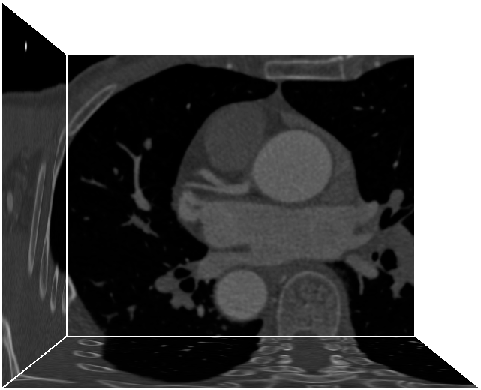
\includegraphics[width=2.8in]{Figures/chap04/original.png}
\caption{Original ROI-extracted volumetric data}
\label{fig:Original}
\end{figure}
\begin{figure}[t]
\centering
\subfloat[]{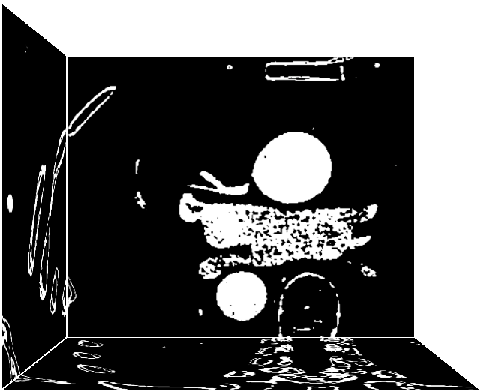
\includegraphics[width=2.8in]{Figures/chap04/binary1.png}%
\label{fig:Binary1}}
\hfil
\subfloat[]{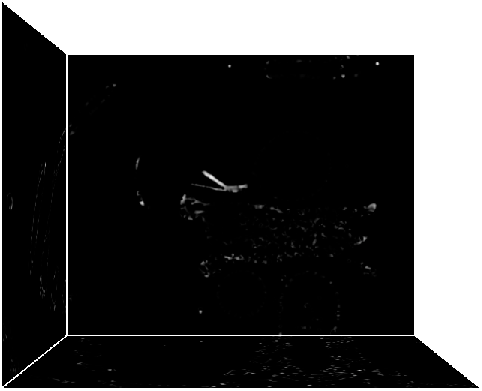
\includegraphics[width=2.8in]{Figures/chap04/hessian.png}%
\label{fig:Vesselness}}
\caption{Preprocessing results of the original CTA images based on the ``vesselness" measure: (a) binary thresholding ($\text{lower threshold} = 300$, $\text{upper threshold} = 600$) (b) tubular enhancement ($\sigma = 0.9$, $\gamma_{12} = 0.1$, $\gamma_{23} = 2.0$).}%
\label{fig:Preprocessing}
\end{figure}

\subsection{Feature Images Computation}

To generate the feature images for the CURVES system, two steps were performed:
(1) calculating the gradient magnitude at each pixel; and
(2) converting the gradient images into the speed images.
%\begin{enumerate}
%\item calculating the gradient magnitude at each pixel;
%\item converting the gradient images into the speed images.
%\end{enumerate}
The gradient magnitude module computed the magnitude of the gradient pixel-wisely for the image by performing the convolution with the first order derivatives of a Gaussian kernel.
The wall of the tiny vessels were extracted before the nonlinear intensity mapping was employed to generate the edge potential maps.
The extreme values of the pixel intensities in the gradient magnitude images directly effected the selection of the parameters in (\ref{eqn:Sigmoid}).
To reverse the lightness of the objects (in low intensities in the gradient magnitude images) and its edges (in high intensities in the gradient magnitude images), $n$ was chosen to be the center of the intensity window containing the vessels, and $m$ a negative value with $|m|$ as the width of the window. %
The minus sign of $m$ means the reverse operation on the pixels.
The neighborhood of the boundaries of the objects were in almost zero intensity, which made the evolution driven by (\ref{eqn:Application}) faster in the ``plateau" (with uniformly high intensities), whilst much slower (in a speed of about zero) in the ``ridges" (with rapid decreasing intensities). %

\subsection{Wave Fronts Propagation}

The initial level sets were evolved by the colliding fronts module.
Two seeds were located interior of the regions corresponding to the coronary arteries and the interfaces surrounding each seeds evolved towards each other.
The dot production of the gradients of arrival times of the two wavefronts were computed.
\begin{figure}[t]
\centering
\subfloat[]{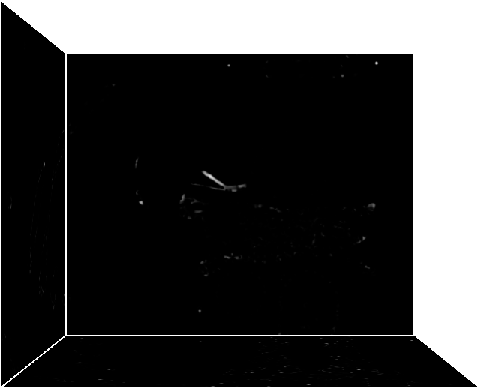
\includegraphics[width=2.8in]{Figures/chap04/sigmoid.png}%
\label{fig:Sigmoid}}
\hfil
\subfloat[]{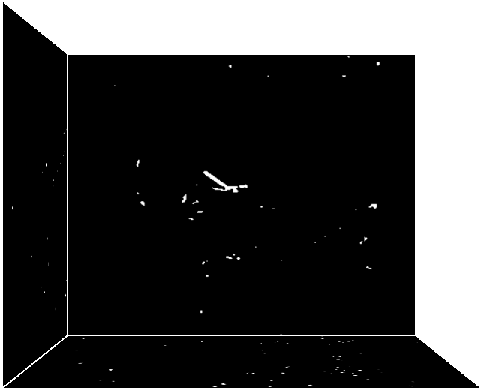
\includegraphics[width=2.8in]{Figures/chap04/binary2.png}%
\label{fig:Binary2}}
\caption{Comparison of the two different intensity conditioning approaches: (a) nonlinear intensity mapping ($m = 80$, $n = 120$); (b) binary thresholding ($\text{lower threshold} = 40$, $\text{upper threshold} = 200$).}%
\label{fig:IntensityConditioning}
\end{figure}
\begin{figure}[t]
\centering
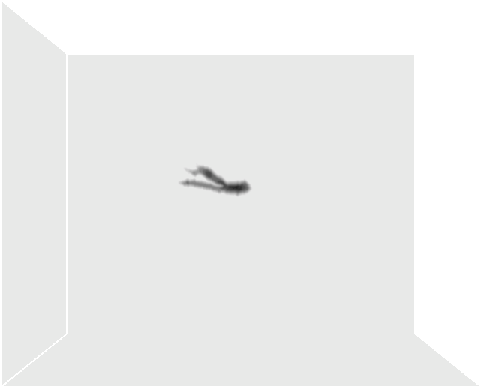
\includegraphics[width=2.8in]{Figures/chap04/curves.png}
\caption{CURVES evolution based on the initial contours generated by the colliding fronts method and the edge feature maps calculated by the nonlinear intensity mapping function.}%
\label{fig:CURVES}
\end{figure}
\begin{figure*}[t]
\centering
\subfloat[]{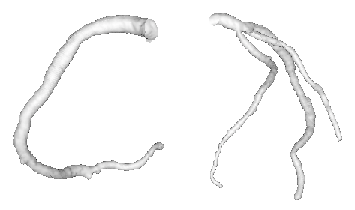
\includegraphics[width=2.8in]{Figures/chap04/model_conventional.png}%
\label{fig:VisualizationModelCURVES}}
\hfil
\subfloat[]{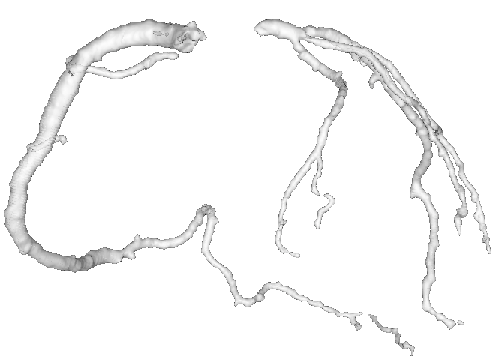
\includegraphics[width=2.4in]{Figures/chap04/model_enhanced.png}%
\label{fig:VisualizationModelTECURVES}}
\caption{Models of the coronary arteries: (a) conventional CURVES evolution; (b) tubular-enhanced CURVES evolution.}%
\label{fig:VisualizationModel}
\end{figure*}

The CURVES system started working when all the preceding calculation completed.
The module took the speed images as its evolution maps and the initial contours as its initial states and regulates the evolution according to (\ref{eqn:Application}).
The evolution terminated when the contours evolved against the wall of the coronary arteries in the specified steps of iterations.
And the resulting evolution extracted the coronary arteries as shown in Fig. \ref{fig:CURVES}.
Next a binary thresholding step was provoked to label the inner area of the coronary arteries with high intensity value whilst the outer area with zero intensity value.

\subsection{Visualization of Segmentation Results}

By manually picked the isovalue corresponding to the wall of the coronary arteries, the resulting volume were processed using the marching cubes method \cite{Lorensen1987MC}.
The visualization models of the coronary arteries respectively based on the CURVES regions without and with tubular enhancement demonstrated their capabilities of displaying the complicated geometrical details (see Fig. \ref{fig:VisualizationModelCURVES} and \ref{fig:VisualizationModelTECURVES}). %

%# -*- coding:utf-8 -*-
\section{Conclusions and Future Work}
\label{sec4_3}
%The conclusion goes here.

The three dimensional visualization of the blood vessels plays an important role in the construction of the virtual scenario for the robotic surgical simulator.
Further, the visualization of the coronary arteries is the most critical and difficult work.
Because of the complex spatial topologies, details can be easily lost in the process of segmentation.
In this paper, a vasculature segmentation method based on tubular-enhanced CURVES has been developed.
Then the process of the experiment was presented and the results were demonstrated.
The experimental results showed that the proposed approach is capable of enhancing the tiny dark vessels and visualizing the geometric details of them.

The tubular feature of coronary arteries was enhanced and the speed images were generated.
Meanwhile, the initial contours for the CURVES method were computed by a modified version of fast marching method in another process.
The actual level sets evolution began after the above computation finished and the evolution took a specified number of iterations to detect the coronary arteries.
At the end of the segmentation, the resulting pixels were all conversed in their intensities.
Finally the data representing the surface of the arteries was extracted by the marching cubes method.

Our future plans are the further optimization of the blood vessel models for the simulation with virtual tools of the robotic surgical simulator.
The principle work will be the decimation of the quantity of the triangles consisting the blood vessels and the improvements of the visualization effects of the virtual scenario. 

%# -*- coding:utf-8 -*-
\chapter{血管模型中心线的提取}
\label{chap5}

%# -*- coding:utf-8 -*-

%Cardiovascular diseases are among the most fatal illnesses in the world.
%Percutaneous coronary intervention is the gold standard in the past decades due to the much less trauma and quick recovery.
%On the other hand, for the guidance of the fluoroscope required by the procedure, the clinicians have to suffer high risks of tumors and other diseases.
%Intravascular robotic systems are applied to change this situation.
%Hence the clinicians need to participate full training projects to ensure the flexible manipulation of the systems.
The computer-aided surgical simulation aims to provide an economic tool of effectiveness and convenience for the training process.
In building this simulation system, the construction of the virtual anatomic environment is one of the major tasks.
It provides the virtual tools with the scenario in which they are manipulated by the trainee.
In intravascular surgery simulation, the surface model of the blood vessels is the most important part of the virtual environment.
In order to achieve better performances in the simulation of path planning and navigation, the surface model based on real patient's CTA data needs further process.
We proposed in this paper an approach to extract the centerlines of each segment of the image-based surface model of the blood vessels.
The surface model is firstly processed to check the connectivity of the consisting polygons in order to extract the largest connected region within the surface.
Next, the resulting surface is smoothed by a windowed sinc function kernel with proper parameters.
After the normal vectors of the smoothed surface are computed, the surface is subdivided and the centerlines of the surface model are computed by using the power crust algorithm. %
The experimental results show that the approach is capable of extracting the centerlines of the vessel model.

\section{Introduction}
\label{sec5_0}
% no \PARstart
Cardiovascular diseases are among the most fatal illnesses worldwide \cite{WHO2013}.
The diseases occur when the stenosis or even blockages formed due to the build up of fatty substances on the inner wall of the blood vessels.
Percutaneous coronary intervention (PCI) is the gold standard in fighting the lethal diseases.
Due to its minimally-invasive nature, this procedure only causes small incision and much less trauma to the patients.
In addition, the hospitalization after the procedure is in turn dramatically shortened.
However, due to the very nature of minimally-invasiveness of PCI and the complex anatomic structure of the blood vessels, the learners need thorough and strict training before performing the procedure in action. %
What's worse, the practitioners in catheterization labs have to expose themselves under the ionizing radiation from the fluoroscope while examining the morphologies of the patients' vasculature. %

The surgical robotic systems for intravascular procedures have greatly changed this situation.
With the assistance of the robotic systems, cardiology practitioners need not to be worried about the radioactive exposure and the relative risks any more.
Like their ancestors (i.e., the traditional PCI procedure), the skills of manipulating the robotic system to do the surgery are also not easy for the junior residences and still require strict and sufficient training before applying the procedure on the real patients. %

The traditional ways of training PCI procedure are deeply rooted in the physical fashion, i.e., employing biological models (e.g. human cadavers and living animals) or non-biological models (e.g. phantoms). %
The former are disposable and ethic-disputed; let alone the tremendous expenditure on the preservation and feeding, and the distinction in anatomy between human and animal volunteer. %
The latter are stiff and lack of sufficient anatomic details, even though they can be used repeatedly.
Indeed, it is infeasible to conduct the training on the expensive robotic systems whilst ignoring the real needs in the catheterization labs.
To streamline the training and the practice of robotic PCI procedure, a well-designed computing simulation system is required.

The aim of our effort is to provide a training tool of convenience and effectiveness for the minimally-invasive intravascular robotic system \cite{Ji2011EMBC}.
In constructing this training vehicle, the anatomic structures in computing environment especially the vascular system are definitely one of the most substantial components.
The centerlines is an effective way of describing the shape of the model \cite{Ogniewicz1995}, which will provide accurate shape description for the path planning in interactive simulation.
In this paper, we developed an automatic approach based on the Voronoi diagram \cite{Antiga2003} to extract the centerlines of the vasculature.
The input of the proposed approach is the patient-specific image-based surface model of the vasculature, which is reconstructed by applying our previous work \cite{Yang2014ICRA}. %
Before computing the Voronoi diagram of the tubular surface model, several preprocessing should be performed.
First, the connectivity of the polygons that consisting the surface is validated thoroughly to include the largest connected polygons that is effective in representing the surface. %
Second, the bumpy and crusty surfaces are smoothed in order to reduce the effects on the computation of centerlines.
Third, the surfaces are subdivided to gain a more precise geometric feature.
Finally, the centerlines of the vessel model by solving the Eikonal equation in the fast marching flavor.
The capability of our approach in automatically extracting the centerlines of the vessel model is proved by the experimental results.

The rest of this paper is organized as follows.
Section II introduces the related work of the centerline extraction methods for three dimensional objects.
Section III outlines the work flow and describes the techniques used in this work.
Section IV describes the experiments, ending with a brief discussion.
The final section concludes the whole work. 
%# -*- coding:utf-8 -*-
\section{Related Work}
\label{sec5_1}

Many researches have been done since the earliest work on extracting the centerline was proposed by Blum \cite{Blum1967}.
According to reference \cite{Ogniewicz1995}, most of these methods fall into four categories: (1) topological thinning; (2) distance transformation; (3) ``prairie fire" approach; (4) Voronoi Diagram methods. %

Topological thinning methods \cite{Ma2002,Sadleir2002} implement the centerline extraction by iteratively remove most of the ``simple points" except the ones that are the end-points of the generated centerline models. %
By ``simple points", it means that the boundary points consisting the object such that their removals do not destroy the topology of the object.

Distance transformation methods \cite{Niblack1992} find the centerline by searching the local maximum among the minimal distances between the points interior of the shape and the boundary. %
However, they do not ensure the resulting centerlines are connected with each other.

``Prairie fire" methods \cite{Blum1967,Leymarie1992} compute the centerline by determining the intersection of the propagating interfaces with their sources located on the boundary of the shape. %

Voronoi diagram method \cite{Sherbrooke1996,Antiga2003} treats the centerline to be generated as a subset of the Voronoi diagram.
These methods are sensitive to the noises and the regularization of the boundary of the shape.

There are numbers of other methods that are not belong to any category listed above.
Ferchichi and Wang in \cite{Ferchichi2006} reported a clustering-based algorithm for centerline extraction both for 2D and 3D objects.
The algorithm was designed based on the idea of computing the maximal disks/balls determining the centerlines, which is achieved by executing the K-means algorithm iteratively on the object-points and their distance transforms. %
Egger \textit{et al.} \cite{Egger2007} reported a centerline extraction algorithm for the blood vessels using Dijkstra's shortest path algorithm, which was designed for the catheter simulation. %
\section{Related Work}

Many researches have been done since the earliest work on extracting the centerline was proposed by Blum \cite{Blum1967}.
According to reference \cite{Ogniewicz1995}, most of these methods fall into four categories: (1) topological thinning; (2) distance transformation; (3) ``prairie fire" approach; (4) Voronoi Diagram methods. %

Topological thinning methods \cite{Ma2002,Sadleir2002} implement the centerline extraction by iteratively remove most of the ``simple points" except the ones that are the end-points of the generated centerline models. %
By ``simple points", it means that the boundary points consisting the object such that their removals do not destroy the topology of the object.

Distance transformation methods \cite{Niblack1992} find the centerline by searching the local maximum among the minimal distances between the points interior of the shape and the boundary. %
However, they do not ensure the resulting centerlines are connected with each other.

``Prairie fire" methods \cite{Blum1967,Leymarie1992} compute the centerline by determining the intersection of the propagating interfaces with their sources located on the boundary of the shape. %

Voronoi diagram method \cite{Sherbrooke1996,Antiga2003} treats the centerline to be generated as a subset of the Voronoi diagram.
These methods are sensitive to the noises and the regularization of the boundary of the shape.

There are numbers of other methods that are not belong to any category listed above.
Ferchichi and Wang in \cite{Ferchichi2006} reported a clustering-based algorithm for centerline extraction both for 2D and 3D objects.
The algorithm was designed based on the idea of computing the maximal disks/balls determining the centerlines, which is achieved by executing the K-means algorithm iteratively on the object-points and their distance transforms. %
Egger \textit{et al.} \cite{Egger2007} reported a centerline extraction algorithm for the blood vessels using Dijkstra's shortest path algorithm, which was designed for the catheter simulation. %

%# -*- coding:utf-8 -*-
\section{Methodologies}
\label{sec5_3}

This section discusses the design of the processing pipeline and details the principles of the consisting modules.
Before the actual centerline extraction begins, several processing aims to removing noises and smoothing the irregular surfaces need to be run to guarantee the quality of the input surface.
The image-based surface model of the blood vessels needs series of postprocessing steps depicted in Fig. \ref{fig:DataFlow} to meet the requirements of the centerline computing module. %
Among these processing steps, the first one is the validation of the connectivity of the consisting polygons.
During this process, the largest possible connected regions of the surface model are extracted.
Next, the surface smoothing step is needed to depress the ``crusts" and ``stairs" in the surface.
Then the normal vectors (i.e., normals) are computed to mark the ``inside" and the ``outside" of the surface model.
After that, the consisting polygons need to be subdivided under a specified criterion to facilitate the computation of the centerline extraction at the cost of longer computation time. %

%\subsection{Processing on Image-Based Surface Model}

\subsection{Connectivity Validation and Largest Region Extraction}

In this paper, the vasculature surface model is generated from the original medical volumetric data set by applying the approaches reported in our previous work \cite{Yang2014ICRA}. %
In order to find the largest region spanning the surface of the vasculature, the connectivity among the vertices in the image-based surface model needs to be thoroughly validated at the beginning of the processing. %
The inner working is to extract consisting polygons that share common vertices and meet some requirements.
In the present paper we implement the algorithm to extract the largest connected region from the input surface.
\begin{figure}[t]
\centering
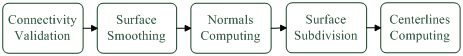
\includegraphics[width=3.2in]{Figures/chap05/DataFlow.png}
\caption{Overview of the work flow.}
\label{fig:DataFlow}
\end{figure}

\subsection{Surface Smoothing and Normals Computing}

There are plenty of methods used for the surfaces smoothing in visualization.
To overcome the ``facets" by-produced during this approximation, an optimal surface smoothing algorithm treating this problem as low-pass filtering by extending Fourier analysis is adopted \cite{Taubin1996}. %
The adopted method is built upon the formulation of the \emph{discrete graph signals}, which means the functions based on directed graph.
The directed graph $G$ represents the polyhedral surfaces in this problem, which is denoted as the set $\left\{ 1, \ldots, n \right\}$ of nodes with a set of neighborhoods $\left\{ i^{\ast}: i = 1, \ldots, n \right\}$ of node $i$. %
A discrete graph signal can be represented as a vector $x = \left[ x_1, \ldots, x_n \right]^T$, where each component of the vector corresponds one node of the graph.
A polyhedral surface $S = \{ V, F \}$ of $n$ vertices can be treated as a directed graph, where the vertices $V$ corresponds the set of nodes $n$ and the faces $F$ the polygons formed by connected nodes. %

The discrete surface signal, the discrete graph signal defined on the associated graph, can be visualized as a piece-wise linear function defined on the surface.
The computation of the Discrete Fourier Transform (DFT) of the discrete surface signal defined on the surface is achieved by decomposing the surface signals as a linear combination of the eigenvectors of the Laplacian: %
\begin{equation}
\label{eqn:Laplacian}
\Delta x_i = \sum_{j \in i^{\ast}} w_{ij} \left( x_j - x_i \right),
\end{equation}
where $w_{ij}$ is the positive weight for each difference of $x_j - x_i$ and for a given vertex $i$, the sum of its weights are always one.
The matrix form of (\ref{eqn:Laplacian}) is
\begin{equation}
\label{eqn:LaplacianMatrix}
\Delta x = - K x,
\end{equation}
where $K = I - W$, with $I$ an identity matrix and $W$ the matrix of weights $w_{ij}$.

Choosing $0 \leq k_1 \leq \ldots \leq k_n \leq 2 $ as the eigenvalues of $K$, $r_1, \ldots, r_n$ the corresponding right eigenvectors, and $d_1, \ldots, d_n$ the associated dual basis of these eigenvectors, the above $K$ can be obtained as $K = \sum_{i} k_i r_i d_i^T$. %
%\begin{equation}
%\label{eqn:K}
%K = \sum_{i} k_i r_i d_i^T.
%\end{equation}
Thus there is a unique decomposition the discrete graph signal $x$, which can be obtained as a linear combination of the right eigenvectors $x = \sum_{i} \hat{x}_i r_i$, %$r_1, \ldots, r_n$
%\begin{equation}
%\label{eqn:x}
%x = \sum_{i} \hat{x}_i r_i,
%\end{equation}
where $\hat{x}_i = d_i^T x$ is the DFT of $x$.

According to signal processing theory, the filtering calculation on the signal $x$ is to change its frequency distribution at the reference of a transfer function $f$:
\begin{equation}
\bar{x} = \sum_{i} f(k_i) \hat{x}_i r_i = \left( \sum_{i} f(k_i) r_i d_i^T \right) x.
\end{equation}
The \emph{low-pass filtering} mechanism can be implemented by adjusting the weights in the following polynomial approximation
\begin{equation}
\label{eqn:Approximation}
f_{N}(k) = w_0 \frac{\theta}{\pi} T_0 (1 - k / 2) + w_n \sum_{n} \frac{2 \sin (n \theta)}{n \pi} T_n(1 - k / 2),
\end{equation}
where $\theta$ is the unique solution of $k = 2 (1 - \cos \theta)$ on $[0, \pi / 2]$, and $T$ the Chebyshev polynomial.
Here in this paper, the weights in (\ref{eqn:Approximation}) is adjusted to form a Hamming window, among sorts of them, which is demonstrated as follows:
\begin{equation}
\label{eqn:HammingWindow}
w_n = 0.54 + 0.46 \cos (n \pi / (N + 1) ).
\end{equation}

The normal vectors to the surfaces are computed after the surfaces are smoothed.

\subsection{Surface Subdivision}

A modified butterfly scheme for surface subdivision is used in order to refine the smoothed surface model \cite{Zorin1996}.
This scheme is designed in the flavor of interpolating and has been proved to be useful in the circumstances of subdivision for the complex especially irregular surfaces.
The ultimate goal is to improve the visualization of the input surface model without affecting its original shape.
The scalar value associated with the new vertex of the 2-dimensional triangulation is generated by calculating weighted sum of neighboring vertices using the proposed interpolation scheme. %
These vertices located in the neighborhood form the subdivision stencil, which determines the features of the scheme.
By analyzing the stencil, the scheme can quickly identify the relationship between the new vertex and the topology of its neighborhood.
The two most important cases in the surface are the regular sites and the extraordinary sites.
Once the initial subdivision cycles completed, the largest number of the vertices possessing the valence other than six is not exceeding one.
The new scalar value for the midpoint on each edge of the triangulation is calculated by the subdivision scheme falls into the following cases:
(1) edge connects two regular vertices;
(2) edge connects an extraordinary vertex and a regular vertex;
(3) edge connects two extraordinary vertices; and
(4) boundary edges.
%\begin{itemize}
%\item edge connects two regular vertices;
%\item edge connects an extraordinary vertex and a regular vertex;
%\item edge connects two extraordinary vertices;
%\item boundary edges.
%\end{itemize}
Among the above cases, only the first one belongs to the regular case, whilst the rest belong to the extraordinary case.

\subsection{Centerlines Extraction}

Centerlines, or medial axis, can be generally defined as the loci of the centers of the maximal inscribed disks (in 2D space) or spheres (in 3D space) inside an object.
Conversely, the envelop of all maximal inscribed disks/spheres is the boundary/surface of the object that contains these disks/spheres \cite{Amenta2001}.
Our approach employed the method demonstrated in \cite{Antiga2003}, which treats the centerlines as the minimal action paths on the Voronoi diagrams inside the model surface.
The Voronoi diagrams are the discrete approximation of the medial axis of the shape in two or three dimensional space.
The minimization of the line integral of the action path, which links two vertices in the Voronoi diagram, generates the center points that locally maximize their minimal distances to the boundary of the surface.
To do this, the method firstly computes the following Eikonal equation from a given starting point located on the Voronoi diagram
\begin{equation}
\label{eqn:Voronoi}
\left| \nabla T \right| = \frac{1}{R(u)},
\end{equation}
where $T$ marks the time of arrival, $R$ the radius of the maximal inscribed sphere at the time $T$, and $u$ the parametric space of the Voronoi diagram.
Then the centerline is obtained by calculating the following equation upon the previously demonstrated computation terminated:
\begin{equation}
\label{eqn:Centerlines}
\frac{dc}{ds} = - \nabla T,
\end{equation}
where $c$ denotes the centerlines, and $s$ the parametric space of $c$.
As a matter of fact, computation illustrated by (\ref{eqn:Centerlines}) is equivalent to finding the resulting centerline by applying the steepest descent method at each point on the Voronoi diagram.

\section{Experiments and Discussions}

\subsection{Data and Experimental Setup}

The vasculature surface models were generated by applying the approaches proposed in \cite{Yang2014ICRA} from the original CTA images acquired from some real patient.

In our experiments, the programs written in C++ ran on a desktop with Intel's 2.83GHz Core 2 Quad CPU and 4GB RAM.
%For the simplicity of description, part of the abdominal aorta is chopped off to serve as the sample data in our experiments described here (see Fig. \ref{fig:VOI}). %
Part of the abdominal aorta was chopped off to serve as the sample data in our experiments described here (see Fig. \ref{fig:VOI}). %
The approach can be applied straightly to the surface model of the whole abdominal aorta (see Fig. \ref{fig:OverlayGlobal}). %and Fig. \ref{fig:VisualizationModel}).
\begin{figure}[t]
\centering
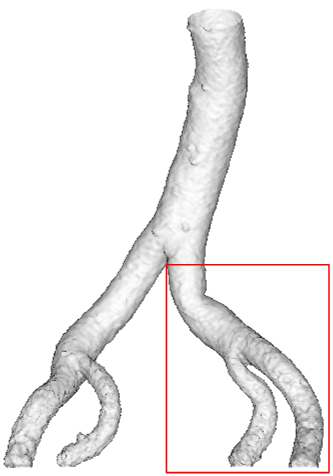
\includegraphics[height=2.4in]{Figures/chap05/VOI.png}
\caption{The original model surface (consists of $205,590$ polygons) and the VOI-extracted local part (in red square).}
\label{fig:VOI}
\end{figure}

%\subsection{Preprocessing for Centerline Extraction}

\subsection{Validating Connectivity of Image-Based Surface Model}

Before actually extracting the centerlines, the image-based surface model of the vasculature needs to be properly conditioned such that the computation can be operated successfully. %
The initial pass is the validation of the connectivity among the adjacent polygonal surfaces that consists of the whole visualization model.
The aim of this step is to find and connect the largest connected region in the given surface model (see Fig. \ref{fig:ConnectivityLocal}).
Table \ref{tbl:Connectivity} shows that the quantities of the consisting polygonal surfaces were not changed in local cases, whilst were decreased in global cases.
The former implies that the given (local) model was the largest connected region in the surface model before the validation.
The latter indicates that the largest connected region of the given model surface was fully extracted through the validation.
\begin{figure}[t]
\centering
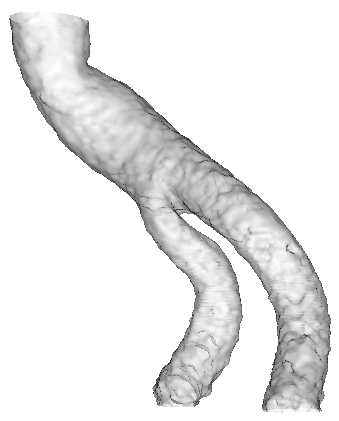
\includegraphics[width=1.5in]{Figures/chap05/connectivity_local.png}
\caption{Results of connectivity validation of model surface in local details (quantity of consisting polygons: $70,625$).}
\label{fig:ConnectivityLocal}
\end{figure}

\begin{table}[t]
\renewcommand{\arraystretch}{1.3}
\caption{Quantities of polygons before and after connectivity validation}
\label{tbl:Connectivity}
\centering
\begin{tabular}
{@{}llr@{}}
%{@{}llrr@{}}
\toprule
%\hline
%~      & ~                       & \multicolumn{2}{c}{Quantities} \\
%\cmidrule(4){3-4}
%~      & ~                       & Vertices & Polygons            \\
~      &                         & Quantities of polygons \\
%\midrule
\hline\hline
%Local  & Before validation       & N/A      & 70,625  \\
%~      & After validation        & N/A      & 70,625  \\
Local  & Before validation       & $70,625$  \\
~      & After validation        & $70,625$  \\
\hline\hline
%Global & Before validation       & N/A      & 205,590 \\
%~      & After validation        & N/A      & 205,452 \\
Global & Before validation       & $205,590$ \\
~      & After validation        & $205,452$ \\
\bottomrule
%\hline
\end{tabular}
\end{table}
\begin{figure}[t]
\centering
\subfloat[]{\includegraphics[width=1.5in]{Figures/chap05/smooth_30_1_local.png}%
\label{fig:Smooth30-1Local}}
\hfil
\subfloat[]{\includegraphics[width=1.45in]{Figures/chap05/smooth_30_01_local.png}%
\label{fig:Smooth30-01Local}}
\hfil
\subfloat[]{\includegraphics[width=1.5in]{Figures/chap05/smooth_100_1_local.png}%
\label{fig:Smooth100-1Local}}
\hfil
\subfloat[]{\includegraphics[width=1.45in]{Figures/chap05/smooth_100_01_local.png}%
\label{fig:Smooth100-01Local}}
\caption{Smoothing effects by applying different parameters: (a) $\text{pass band} = 0.1$, $\text{iterations} = 30$; (b) $\text{pass band} = 0.01$, $\text{iterations} = 30$; (c) $\text{pass band} = 0.1$, $\text{iterations} = 100$; (d) $\text{pass band} = 0.01$, $\text{iterations} = 100$.}%
\label{fig:SmoothLocal}
\end{figure}

%\begin{table}
%\renewcommand{\arraystretch}{1.3}
%\caption{Comparison of quantities of polygonal surfaces - Part I}
%\label{tbl:Eigenvalues}
%\centering
%\begin{tabular}{l||r}
%\hline
%\bfseries Connectivity validation & \bfseries Quantities \\
%\hline\hline
%Before                            & 757,538 \\
%After                             & 757,400 \\
%\hline
%\end{tabular}
%\end{table}

\subsection{Smoothing Connected Surface Model}

The centerline extracting method adopted in this work is sensitive to the noises on the input surface.
Due to the poor quality in some level of details of the original images, segmentation may introduce unnecessary uneven surfaces.
These artifacts in the surfaces can cause difficulties in the delivering of the virtual guidewires towards the hesion along the lumen of the model vessels.
To depress the noisy surface of the model, a surface smoothing module implemented based on low-pass filtering is applied.
There are two parameters associated with the smoothing module.
One of them specifies the number of iterations, which is equivalent to the degree of the polynomial approximating the windowed sinc function defined by (\ref{eqn:Approximation}).
The other determines the pass band of this low-pass filtering module.
Different sets of parameters were fed to the smoothing module in order to find the best results for the following processing (see Fig. \ref{fig:SmoothLocal}).
Observing these results, the parameters ($\text{pass band} = 0.01$, $\text{iterations} = 100$) used to generating the resulting surface in Fig. \ref{fig:Smooth100-01Local} demonstrated better effects than the rest.
%\begin{figure}[t]
%\centering
%\subfloat[]{\includegraphics[width=1.5in]{../Figures/smooth_30_1_local.eps}%
%\label{fig:Smooth30-1Local}}
%\hfil
%\subfloat[]{\includegraphics[width=1.45in]{../Figures/smooth_30_01_local.eps}%
%\label{fig:Smooth30-01Local}}
%\hfil
%\subfloat[]{\includegraphics[width=1.5in]{../Figures/smooth_100_1_local.eps}%
%\label{fig:Smooth100-1Local}}
%\hfil
%\subfloat[]{\includegraphics[width=1.45in]{../Figures/smooth_100_01_local.eps}%
%\label{fig:Smooth100-01Local}}
%\caption{Smoothing effects by applying different parameters: (a) $\text{pass band} = 0.1$, $\text{iterations} = 30$; (b) $\text{pass band} = 0.01$, $\text{iterations} = 30$; (c) $\text{pass band} = 0.1$, $\text{iterations} = 100$; (d) $\text{pass band} = 0.01$, $\text{iterations} = 100$.}%
%\label{fig:SmoothLocal}
%\end{figure}

\subsection{Subdivision Using Improved Butterfly Scheme}

To further attenuate the effects of noisy surfaces on extraction of centerlines and increase the precision of the centerlines extraction, the number of the polygons consisting the model surface has to be increased.
In order to achieve this, the smoothed surface need to be subdivided without introducing more perturbation.
Figure \ref{fig:SubdivisionLocal} illustrates that the subdivision computation based on the improved butterfly scheme.
At the same time, the quantities of the consisting polygonal surfaces increased substantially after the subdivision complete (see Table \ref{tbl:Subdivision}).
Comparing the quantities of the polygons before and after the subdivision in both cases, the quantities of the resulting polygons are about four times greater than the quantities of the input polygons due to the subdivision scheme employed in this work.
\begin{figure}[t]
\centering
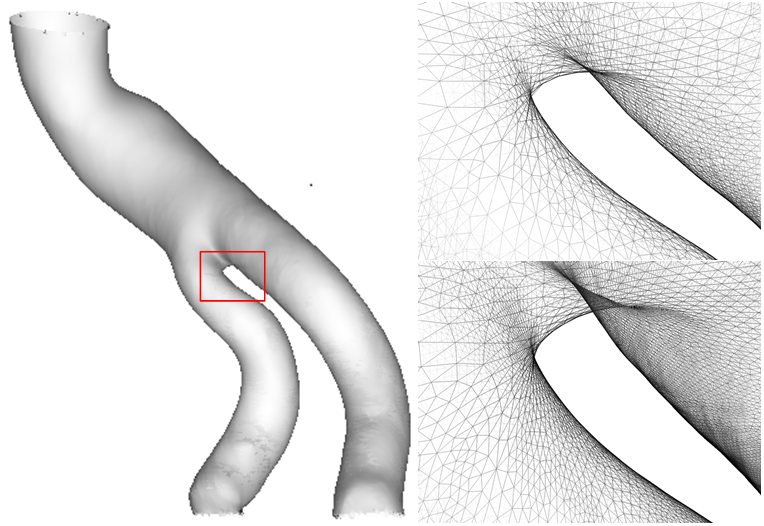
\includegraphics[width=3.0in]{Figures/chap05/subdivision.png}
\caption{Subdivision of smoothed surface by using improved butterfly scheme. \emph{Left}: subdivision in local details. \emph{Top right}: polyhedral surface before subdivision. \emph{Bottom right}: polyhedral surface after subdivision.}%
\label{fig:SubdivisionLocal}
\end{figure}

\begin{table}[t]
\renewcommand{\arraystretch}{1.3}
\caption{Quantities of polygons before and after subdivision using an improved butterfly scheme}
\label{tbl:Subdivision}
\centering
\begin{tabular}
%{@{}llr@{}}
{@{}llrr@{}}
\toprule
%\hline
%~      & ~                       & \multicolumn{2}{c}{Quantities} \\
%\cmidrule(4){3-4}
%~      & ~                       & Vertices & Polygons            \\
~      &                         & Quantities of polygons & Percentages ($\%$)\\
%\midrule
\hline\hline
%Local  & Before subdivision      & N/A      &  70,625  \\
%~      & After subdivision       & N/A      & 281,060  \\
Local  & Before subdivision      &  $70,625$  &\\
~      & After subdivision       & $281,060$  & 398 \\
\hline\hline
%Global & Before validation       & N/A      & 205,452  \\
%~      & After validation        & N/A      & 821,808  \\
Global & Before validation       & $205,452$  &\\
~      & After validation        & $821,808$  & 400 \\
\bottomrule
%\hline
\end{tabular}
\end{table}

%\begin{table}
%\renewcommand{\arraystretch}{1.3}
%\caption{Comparison of quantities of polygonal surfaces - Part II}
%\label{tbl:Eigenvalues}
%\centering
%\begin{tabular}{l||r}
%\hline
%\bfseries Subdivision  & \bfseries Quantities \\
%\hline\hline
%Before                 &  757,400 \\
%After                  & 3,029,600 \\
%\hline
%\end{tabular}
%\end{table}

\begin{figure}[t]
\centering
\subfloat[]{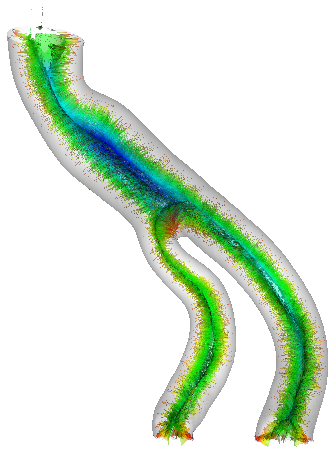
\includegraphics[width=1.5in]{Figures/chap05/overlay_100_01_voronoi_local.png}%
\label{fig:VoronoiLocal}}
\hfil
\subfloat[]{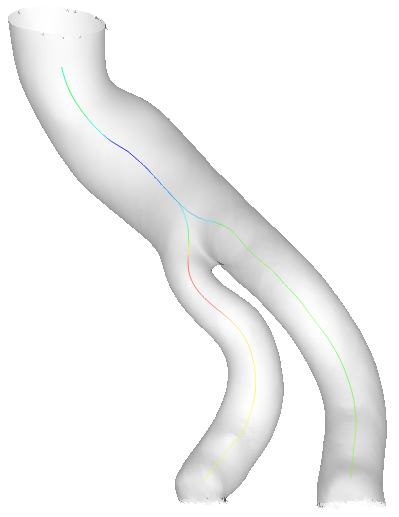
\includegraphics[width=1.5in]{Figures/chap05/overlay_100_01_centerlines_local.png}%
\label{fig:OverlayLocal}}
\caption{Centerlines extraction of the aorta in local details: (a) embedded Voronoi diagram; (b) centerlines inside the vessel.}%
\label{fig:CenterlinesLocal}
\end{figure}

\begin{figure}[t]
\centering
\subfloat[]{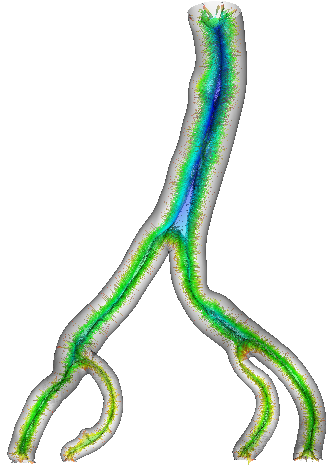
\includegraphics[height=2.0in]{Figures/chap05/overlay_100_01_voronoi.png}
%\caption{Voronoi diagrams of the abdominal aorta.}
\label{fig:VoronoiGlobal}}
\hfil
\subfloat[]{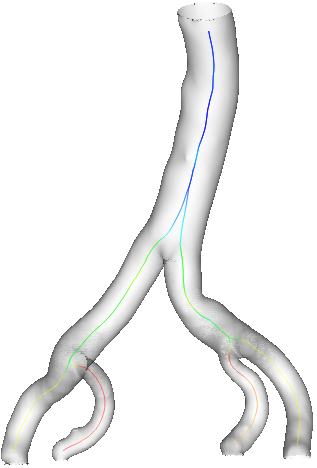
\includegraphics[height=2.0in]{Figures/chap05/overlay_100_01_centerlines.png}
%\caption{Centerlines of the abdominal aorta.}
\label{fig:OverlayGlobal}}
\caption{Centerlines extraction of the aorta in VOI. (a) Voronoi diagrams; (b) Centerlines. }
\label{fig:CenterlineGlobal}
\end{figure}

\subsection{Centerlines Extraction Based on Surface Model}

The centerlines extraction computation was performed on the subdivided surface model.
Firstly, the embedded Voronoi diagram of the preprocessed surface model is generated (see Fig. \ref{fig:VoronoiLocal}).
Secondly, the centerlines of the tubular surface model is computed (see Fig. \ref{fig:OverlayLocal}).
The colors marked on the Voronoi diagram and the centerlines denote the diameters of the local resection circle, decreasing from blue to red.
The same processing was straightly applied to the model surface of the whole abdominal aorta (see Fig. \ref{fig:VoronoiGlobal} and Fig. \ref{fig:OverlayGlobal}).
One can see from the details of the results that the starting and ending points are not exactly located at the ``entrances" or ``exits".
The reason of this is the Voronoi diagram on which the points consisting the centerlines exist never intersect with the model surface, i.e., the ending points of the centerlines are approaching the terminals of the surface model as near as possible, but never stick to them.
\begin{figure}[t]
\centering
\subfloat[]{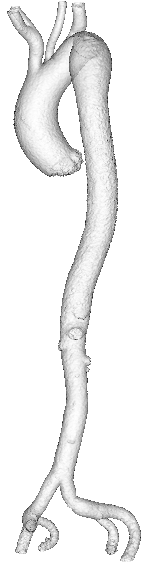
\includegraphics[width=0.7in]{Figures/chap05/surface.png}%
\label{fig:SurfaceModel}}
\hfil
\subfloat[]{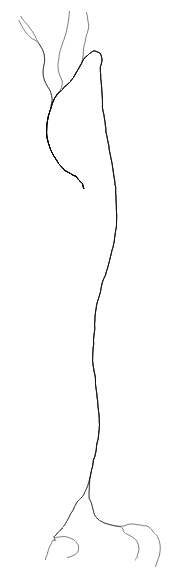
\includegraphics[width=0.9in]{Figures/chap05/centerlines.png}%
\label{fig:CenterlinesModel}}
\caption{Visualization models of the aorta: (a) image-based surface model (quantity of consisting polygons: $757,538$); (b) centerlines of the surface model.}%
\label{fig:VisualizationModel}
\end{figure}

\subsection{Discussions}

The computer programs used in this paper were written in C++ based on the Visualization Toolkit, an open source library aims at providing general facilities in the scientific visualization field \cite{Schroeder2000VTK}. %
To depress the unintended affections of the unstructured polygonal surfaces and the noises introduced by the image segmentation, series of steps were introduced in our experiments to extract the centerlines of the surface model of the vasculature. %
During this process, the quantities of the consisting polygons were obviously decreased for the extraction of the largest connected region in the surface model.
Due to the centerlines extraction computation is sensitive and expensive, we subdivided the smoothed surface model based on an improved butterfly scheme.
After this process, the quantities of the consisting polygonal surfaces were increased because of the refinement of the polygons.
With this step, the potential perturbation was further reduced, leading to much less errors which may occur during the computation of the centerlines extraction.
It is noteworthy that the extraction of centerlines for the model surface is an expensive computation both in time and space.
The calculation of the whole aorta (see Fig. \ref{fig:VisualizationModel}) cost nearly eight hours on our desktop machine with dedicated modification on the code to fit the bulky data into the relatively limited memory. %
%The calculation of the whole aorta cost nearly eight hours on our desktop machine with dedicated modification on the code to fit the bulky data into the relatively limited memory. %

%# -*- coding:utf-8 -*-
\section{Experiments and Discussions}
\label{sec5_3}

\subsection{Data and Experimental Setup}

The vasculature surface models were generated by applying the approaches proposed in \cite{Yang2014ICRA} from the original CTA images acquired from some real patient.

In our experiments, the programs written in C++ ran on a desktop with Intel's 2.83GHz Core 2 Quad CPU and 4GB RAM.
%For the simplicity of description, part of the abdominal aorta is chopped off to serve as the sample data in our experiments described here (see Fig. \ref{fig:VOI}). %
Part of the abdominal aorta was chopped off to serve as the sample data in our experiments described here (see Fig. \ref{fig:VOI}). %
The approach can be applied straightly to the surface model of the whole abdominal aorta (see Fig. \ref{fig:OverlayGlobal}). %and Fig. \ref{fig:VisualizationModel}).
\begin{figure}[t]
\centering
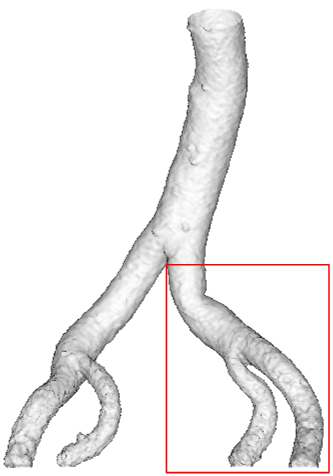
\includegraphics[height=2.4in]{Figures/chap05/VOI.png}
\caption{The original model surface (consists of $205,590$ polygons) and the VOI-extracted local part (in red square).}
\label{fig:VOI}
\end{figure}

%\subsection{Preprocessing for Centerline Extraction}

\subsection{Validating Connectivity of Image-Based Surface Model}

Before actually extracting the centerlines, the image-based surface model of the vasculature needs to be properly conditioned such that the computation can be operated successfully. %
The initial pass is the validation of the connectivity among the adjacent polygonal surfaces that consists of the whole visualization model.
The aim of this step is to find and connect the largest connected region in the given surface model (see Fig. \ref{fig:ConnectivityLocal}).
Table \ref{tbl:Connectivity} shows that the quantities of the consisting polygonal surfaces were not changed in local cases, whilst were decreased in global cases.
The former implies that the given (local) model was the largest connected region in the surface model before the validation.
The latter indicates that the largest connected region of the given model surface was fully extracted through the validation.
\begin{figure}[t]
\centering
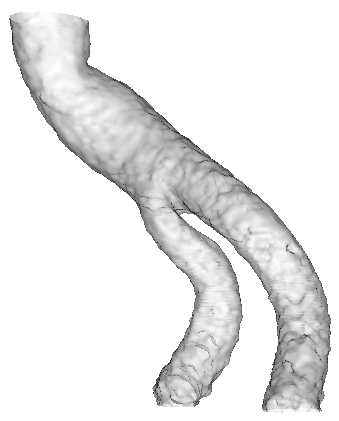
\includegraphics[width=1.5in]{Figures/chap05/connectivity_local.png}
\caption{Results of connectivity validation of model surface in local details (quantity of consisting polygons: $70,625$).}
\label{fig:ConnectivityLocal}
\end{figure}

\begin{table}[t]
\renewcommand{\arraystretch}{1.3}
\caption{Quantities of polygons before and after connectivity validation}
\label{tbl:Connectivity}
\centering
\begin{tabular}
{@{}llr@{}}
%{@{}llrr@{}}
\toprule
%\hline
%~      & ~                       & \multicolumn{2}{c}{Quantities} \\
%\cmidrule(4){3-4}
%~      & ~                       & Vertices & Polygons            \\
~      &                         & Quantities of polygons \\
%\midrule
\hline\hline
%Local  & Before validation       & N/A      & 70,625  \\
%~      & After validation        & N/A      & 70,625  \\
Local  & Before validation       & $70,625$  \\
~      & After validation        & $70,625$  \\
\hline\hline
%Global & Before validation       & N/A      & 205,590 \\
%~      & After validation        & N/A      & 205,452 \\
Global & Before validation       & $205,590$ \\
~      & After validation        & $205,452$ \\
\bottomrule
%\hline
\end{tabular}
\end{table}
\begin{figure}[t]
\centering
\subfloat[]{\includegraphics[width=1.5in]{Figures/chap05/smooth_30_1_local.png}%
\label{fig:Smooth30-1Local}}
\hfil
\subfloat[]{\includegraphics[width=1.45in]{Figures/chap05/smooth_30_01_local.png}%
\label{fig:Smooth30-01Local}}
\hfil
\subfloat[]{\includegraphics[width=1.5in]{Figures/chap05/smooth_100_1_local.png}%
\label{fig:Smooth100-1Local}}
\hfil
\subfloat[]{\includegraphics[width=1.45in]{Figures/chap05/smooth_100_01_local.png}%
\label{fig:Smooth100-01Local}}
\caption{Smoothing effects by applying different parameters: (a) $\text{pass band} = 0.1$, $\text{iterations} = 30$; (b) $\text{pass band} = 0.01$, $\text{iterations} = 30$; (c) $\text{pass band} = 0.1$, $\text{iterations} = 100$; (d) $\text{pass band} = 0.01$, $\text{iterations} = 100$.}%
\label{fig:SmoothLocal}
\end{figure}

%\begin{table}
%\renewcommand{\arraystretch}{1.3}
%\caption{Comparison of quantities of polygonal surfaces - Part I}
%\label{tbl:Eigenvalues}
%\centering
%\begin{tabular}{l||r}
%\hline
%\bfseries Connectivity validation & \bfseries Quantities \\
%\hline\hline
%Before                            & 757,538 \\
%After                             & 757,400 \\
%\hline
%\end{tabular}
%\end{table}

\subsection{Smoothing Connected Surface Model}

The centerline extracting method adopted in this work is sensitive to the noises on the input surface.
Due to the poor quality in some level of details of the original images, segmentation may introduce unnecessary uneven surfaces.
These artifacts in the surfaces can cause difficulties in the delivering of the virtual guidewires towards the hesion along the lumen of the model vessels.
To depress the noisy surface of the model, a surface smoothing module implemented based on low-pass filtering is applied.
There are two parameters associated with the smoothing module.
One of them specifies the number of iterations, which is equivalent to the degree of the polynomial approximating the windowed sinc function defined by (\ref{eqn:Approximation}).
The other determines the pass band of this low-pass filtering module.
Different sets of parameters were fed to the smoothing module in order to find the best results for the following processing (see Fig. \ref{fig:SmoothLocal}).
Observing these results, the parameters ($\text{pass band} = 0.01$, $\text{iterations} = 100$) used to generating the resulting surface in Fig. \ref{fig:Smooth100-01Local} demonstrated better effects than the rest.
%\begin{figure}[t]
%\centering
%\subfloat[]{\includegraphics[width=1.5in]{../Figures/smooth_30_1_local.eps}%
%\label{fig:Smooth30-1Local}}
%\hfil
%\subfloat[]{\includegraphics[width=1.45in]{../Figures/smooth_30_01_local.eps}%
%\label{fig:Smooth30-01Local}}
%\hfil
%\subfloat[]{\includegraphics[width=1.5in]{../Figures/smooth_100_1_local.eps}%
%\label{fig:Smooth100-1Local}}
%\hfil
%\subfloat[]{\includegraphics[width=1.45in]{../Figures/smooth_100_01_local.eps}%
%\label{fig:Smooth100-01Local}}
%\caption{Smoothing effects by applying different parameters: (a) $\text{pass band} = 0.1$, $\text{iterations} = 30$; (b) $\text{pass band} = 0.01$, $\text{iterations} = 30$; (c) $\text{pass band} = 0.1$, $\text{iterations} = 100$; (d) $\text{pass band} = 0.01$, $\text{iterations} = 100$.}%
%\label{fig:SmoothLocal}
%\end{figure}

\subsection{Subdivision Using Improved Butterfly Scheme}

To further attenuate the effects of noisy surfaces on extraction of centerlines and increase the precision of the centerlines extraction, the number of the polygons consisting the model surface has to be increased.
In order to achieve this, the smoothed surface need to be subdivided without introducing more perturbation.
Figure \ref{fig:SubdivisionLocal} illustrates that the subdivision computation based on the improved butterfly scheme.
At the same time, the quantities of the consisting polygonal surfaces increased substantially after the subdivision complete (see Table \ref{tbl:Subdivision}).
Comparing the quantities of the polygons before and after the subdivision in both cases, the quantities of the resulting polygons are about four times greater than the quantities of the input polygons due to the subdivision scheme employed in this work.
\begin{figure}[t]
\centering
\includegraphics[width=3.0in]{Figures/chap05/subdivision.png}
\caption{Subdivision of smoothed surface by using improved butterfly scheme. \emph{Left}: subdivision in local details. \emph{Top right}: polyhedral surface before subdivision. \emph{Bottom right}: polyhedral surface after subdivision.}%
\label{fig:SubdivisionLocal}
\end{figure}

\begin{table}[t]
\renewcommand{\arraystretch}{1.3}
\caption{Quantities of polygons before and after subdivision using an improved butterfly scheme}
\label{tbl:Subdivision}
\centering
\begin{tabular}
%{@{}llr@{}}
{@{}llrr@{}}
\toprule
%\hline
%~      & ~                       & \multicolumn{2}{c}{Quantities} \\
%\cmidrule(4){3-4}
%~      & ~                       & Vertices & Polygons            \\
~      &                         & Quantities of polygons & Percentages ($\%$)\\
%\midrule
\hline\hline
%Local  & Before subdivision      & N/A      &  70,625  \\
%~      & After subdivision       & N/A      & 281,060  \\
Local  & Before subdivision      &  $70,625$  &\\
~      & After subdivision       & $281,060$  & 398 \\
\hline\hline
%Global & Before validation       & N/A      & 205,452  \\
%~      & After validation        & N/A      & 821,808  \\
Global & Before validation       & $205,452$  &\\
~      & After validation        & $821,808$  & 400 \\
\bottomrule
%\hline
\end{tabular}
\end{table}

%\begin{table}
%\renewcommand{\arraystretch}{1.3}
%\caption{Comparison of quantities of polygonal surfaces - Part II}
%\label{tbl:Eigenvalues}
%\centering
%\begin{tabular}{l||r}
%\hline
%\bfseries Subdivision  & \bfseries Quantities \\
%\hline\hline
%Before                 &  757,400 \\
%After                  & 3,029,600 \\
%\hline
%\end{tabular}
%\end{table}

\begin{figure}[t]
\centering
\subfloat[]{\includegraphics[width=1.5in]{Figures/chap05/overlay_100_01_voronoi_local.png}%
\label{fig:VoronoiLocal}}
\hfil
\subfloat[]{\includegraphics[width=1.5in]{Figures/chap05/overlay_100_01_centerlines_local.png}%
\label{fig:OverlayLocal}}
\caption{Centerlines extraction of the aorta in local details: (a) embedded Voronoi diagram; (b) centerlines inside the vessel.}%
\label{fig:CenterlinesLocal}
\end{figure}

\begin{figure}[t]
\centering
\subfloat[]{\includegraphics[height=2.0in]{Figures/chap05/overlay_100_01_voronoi.png}
%\caption{Voronoi diagrams of the abdominal aorta.}
\label{fig:VoronoiGlobal}}
\hfil
\subfloat[]{\includegraphics[height=2.0in]{Figures/chap05/overlay_100_01_centerlines.png}
%\caption{Centerlines of the abdominal aorta.}
\label{fig:OverlayGlobal}}
\caption{Centerlines extraction of the aorta in VOI. (a) Voronoi diagrams; (b) Centerlines. }
\label{fig:CenterlineGlobal}
\end{figure}

\subsection{Centerlines Extraction Based on Surface Model}

The centerlines extraction computation was performed on the subdivided surface model.
Firstly, the embedded Voronoi diagram of the preprocessed surface model is generated (see Fig. \ref{fig:VoronoiLocal}).
Secondly, the centerlines of the tubular surface model is computed (see Fig. \ref{fig:OverlayLocal}).
The colors marked on the Voronoi diagram and the centerlines denote the diameters of the local resection circle, decreasing from blue to red.
The same processing was straightly applied to the model surface of the whole abdominal aorta (see Fig. \ref{fig:VoronoiGlobal} and Fig. \ref{fig:OverlayGlobal}).
One can see from the details of the results that the starting and ending points are not exactly located at the ``entrances" or ``exits".
The reason of this is the Voronoi diagram on which the points consisting the centerlines exist never intersect with the model surface, i.e., the ending points of the centerlines are approaching the terminals of the surface model as near as possible, but never stick to them.
\begin{figure}[t]
\centering
\subfloat[]{\includegraphics[width=0.7in]{Figures/chap05/surface.png}%
\label{fig:SurfaceModel}}
\hfil
\subfloat[]{\includegraphics[width=0.9in]{Figures/chap05/centerlines.png}%
\label{fig:CenterlinesModel}}
\caption{Visualization models of the aorta: (a) image-based surface model (quantity of consisting polygons: $757,538$); (b) centerlines of the surface model.}%
\label{fig:VisualizationModel}
\end{figure}

\subsection{Discussions}

The computer programs used in this paper were written in C++ based on the Visualization Toolkit, an open source library aims at providing general facilities in the scientific visualization field \cite{Schroeder2000VTK}. %
To depress the unintended affections of the unstructured polygonal surfaces and the noises introduced by the image segmentation, series of steps were introduced in our experiments to extract the centerlines of the surface model of the vasculature. %
During this process, the quantities of the consisting polygons were obviously decreased for the extraction of the largest connected region in the surface model.
Due to the centerlines extraction computation is sensitive and expensive, we subdivided the smoothed surface model based on an improved butterfly scheme.
After this process, the quantities of the consisting polygonal surfaces were increased because of the refinement of the polygons.
With this step, the potential perturbation was further reduced, leading to much less errors which may occur during the computation of the centerlines extraction.
It is noteworthy that the extraction of centerlines for the model surface is an expensive computation both in time and space.
The calculation of the whole aorta (see Fig. \ref{fig:VisualizationModel}) cost nearly eight hours on our desktop machine with dedicated modification on the code to fit the bulky data into the relatively limited memory. %
%The calculation of the whole aorta cost nearly eight hours on our desktop machine with dedicated modification on the code to fit the bulky data into the relatively limited memory. %

%# -*- coding:utf-8 -*-
\section{Conclusions and Future Work}
\label{sec5_4}
%The conclusion goes here.

Centerlines are useful in describing the shape of three dimensional objects.
In implementing the intravascular surgical simulation system, centerlines model of the vasculature will serve as the shape description for the simulation of path planning and navigation of the virtual guidewires/catheters.
In this paper, an automatic approach is designed and validated to extract the centerlines of the image-based patient-specific vasculature model.
The shape analysis presented here lays the foundation for our further research in visualizing the vessels that are closely related to the simulation of PCI procedure.

The connectivity of the polygons in the surface model is firstly checked to find out and remove the redundant polygons that are irrelevant to the actual surface.
Then the resulting surfaces are smoothed at the locations that seems to be uneven in order to prevent these perturbations against the centerlines computation.
After that, the surfaces are subdivided by applying an improved butterfly scheme with the aim of acquiring a more precise surface model.
Finally, the Eikonal equation of the time of arrivals of the embedded Voronoi diagram is computed to obtain the centerlines of the model surface.
Experiments are designed and carried out with the results in demonstrating the effectiveness of the developed approach.

In the future, our research directions are further optimization of the surface model on the one hand, and the visualization of other organs (e.g., heart) and the simulation of the typical phenomena (such as contrast injection, heart beat, etc.) during the procedure on the other. %


%# -*- coding:utf-8 -*-
\chapter{面向虚拟交互的血管模型优化}
\label{chap6}

%# -*- coding:utf-8 -*-

%Cardiovascular diseases are among the most fatal illnesses in the world.
Percutaneous coronary intervention is the gold standard to coronary diseases in the past decades due to much less trauma and quick recovery.
%On the other hand, for the guidance of the fluoroscope required by the procedure, the clinicians have to suffer high risks of tumors and other diseases.
%Intravascular robotic systems are applied to change this situation.
%Hence the clinicians need to participate full training projects to ensure the flexible manipulation of the systems.
However, due to its minimally invasive traits, clinicians have to defeat the difficulties in eye-hand coordination during the procedure, which also makes it a non-trivial task in the training lab. %
The computer-aided surgical simulation is designed to provide a reliable tool for the early stage of the training process.
In this simulation system, the surface model of the vessels contribute the major part in the virtual anatomic environment.
On the other hand, heavy interactions between the virtual surgical tools and the model surface occur during the training.
In order to achieve acceptable performances, the patient-specific vessel surface model needs further process to adapt to this situation.
We proposed in this paper an approach to optimize the meshes that consist the surface model with its application in consideration.
The connectivity of the surface model is firstly checked.
Next a smooth processing is applied without modifying the geometry of the largest-connected surface.
Then the quantities of the polygons consisting the model surface are eliminated both dramatically and appropriately.
Experimental results illustrated the capability of the proposed approach in optimizing the image-based surface model of human vessels.
The resultant surface model can be used as the validation and experimentation involving the virtual surgical tools.

\section{Introduction}
\label{sec6_0}

%Coronary heart diseases () are among the most fatal illnesses worldwide \cite{WHO2013}.
%The diseases occur when the stenosis or even blockages formed due to the build up of fatty substances on the inner wall of the blood vessels.
Percutaneous coronary intervention (PCI) is the gold standard in fighting the coronary heart diseases, which is one of the most lethal diseases in the modern world \cite{WHO2013}. %
Due to the minimally-invasive traits, this procedure causes smaller incision and much less trauma to the patients than open surgery performed in the past.
%In addition, the hospitalization after the procedure is in turn dramatically shortened.
However, this feature also makes it hard for the learners to get used to it.
Besides, after entering the real catheterization labs, the clinicians have to endure the potential occupational hazards year after year \cite{Smilowitz2012}.
%They typically need strict and long term training before performing the procedure on real patient. %
%What's worse, the practitioners in catheterization labs have to expose themselves under the ionizing radiation from the fluoroscope while examining the morphologies of the patients' vasculature. %

In this context, robot-assisted intravascular system came into play with the aim of changing this situation.
With these robots \cite{Beyar2006RNS,Smilowitz2012}, the work load of the cardiologists are dramatically lightened, and the risks of their health are greatly decreased.
However, as their ancient manually performed counterparts, the technique of steering the robotic arms in surgery is still hard for the novice.

Traditional paradigm of PCI training strictly followed the physical fashion -- performing demonstrative procedure on biological or non-biological models \cite{Lunderquist1995,Mori1998}. %
The former materials, including unclaimed cadavers and live animals, are ethic-disputed.
Moreover, the expenditure on the preservation and feeding is high-rising, and the distinction in anatomy between human and animal volunteer is apparent even for the amateur. %
The latter are rigid and stiff both in touching and looking.

In the case of training of robotic systems, one fact is that the advanced robotic systems can not be applied to the training for the health of the clinicians and the lives of the patients will be at risk. %
In order to solve this problem, better training vehicles are required.
Thanks to the advancement of computer hardware, we could employ the greatly improved computer system as the platform, on which the dedicated computer-aided training simulation can be realized. %

Our aim is to implement a computer-aided simulation training system for the minimally-invasive intravascular robotic system built in our lab \cite{Ji2011EMBC}.
In realizing this training platform, the temporal performance of interaction between the anatomic structures in computing environment (e.g., the vascular system) and the virtual surgical tools are undoubtedly of the primary concern. %
In order to improve this performance, the quantity of the consisting polygons needed to be greatly reduced.

In this paper, we developed an approach to substantially eliminate the total number of the polygonal elements of the vasculature model.
As the most popular primitive for the modern computer graphics application, the polygons can be rendered in any standard commercial computer graphics systems.
The fact is that in surface rendering, the more precise the results are, the more polygons are required.
This makes the rendering of the huge amount of polygons occupy too much computation resources, especially the memories.
In the field of medical visualization and simulation, models rendered using surface techniques require even more polygons to capture various of complex and delicate human anatomic structures. %
The decimation algorithm introduced in our work is an application independent method to eliminate the polygons (especially triangles) by performing local operations \cite{Schroeder1992}. %

The input data is the patient-specific surface model of the human vasculature based on the computed tomography angiography (CTA).
Firstly, the connectivity of the polygons that consisting the surface is validated thoroughly to include the largest connected polygons that is effective in representing the surface. %
Secondly, the uneven surfaces are smoothed in order to reduce the unnecessary effects on the following decimation.
Finally, numbers of the component polygons of the vessel model are eliminated.
The capability of our approach in reducing the amount of polygonal components of the vessel model is proved by the experimental results.

The remainder of this paper is organized as follows.
Section II outlines the work flow and describes the techniques introduced in this work.
Section III describes the experiments and presents the results, ending with a discussion.
The final section concludes the whole work and outlooks the future plans. 
%# -*- coding:utf-8 -*-
\section{Methodologies}
\label{sec6_1}

\subsection{Overview}

This section discusses the layout of the main methods used in processing and optimization of the meshes consisting the model surface.
The surface model of the vasculature used in this work was generated from the CTA information which was acquired from some real patient.
In order to put the model into the use of virtual interaction, the amount of information of the model have to be limited because of the constraints of the graphics hardware.
To limit the amount of information is equivalent to eliminate the total number of the polygonal elements that consist the model as much as possible, while preserving the original geometry of the vasculature. %

Some preprocessing steps illustrated in Fig. \ref{fig:DataFlow} are necessary before the elimination of the polygons in the surface.
First of all, the validation of the connectivity among the vertices in the image-based model surface are performed to guarantee that the surface to be processed is complete as a whole and all the vertices are connected. %
Secondly, the smoothing step is introduced in order to depress the bulges and sunken areas in the connected surface.
Finally, the polygonal elements in the surface model are selected and part of them are deleted; the ``holes" left are patched and the geometry of the model is preserved as complete as possible. %

\subsection{Connectivity Validation}

Before any processing steps, one routine must be done to ensure that the surface model considered is well-shaped that no extra polygons exist in defining the same piece of surface.
This routine is designed to extract the polygons based on the geometric connectivity.
Concretely, it can extract the cells (i.e., polygons and/or triangles) that share the common points (i.e., vertices).

\subsection{Surface Smoothing}

In the field of computer graphics and imaging, the visualization of curves and surfaces (both will be referred to as \emph{shapes}) both in two- or three-dimensional space are common, especially for the volumetric data from medical field. %
The computation is in fact the proper approximation of the original shapes by the polygonal curves or polyhedral surfaces.
Typically, artifacts at certain level can be found in the resultant approximating shapes (see Fig. \ref{fig:Artifact}), and can be smoothed while maintaining the overall geometry (see Fig. \ref{fig:ArtifactRemoved}). %
In this work, one of our objectives is the smoothing or fairing of the model surface acquired by applying the iso-intensity extraction techniques on the raw medical images.
\begin{figure}[t]
\centering
\includegraphics[width=3.2in]{Figures/chap06/DataFlow.png}
\caption{Overview of the work flow.}
\label{fig:DataFlow}
\end{figure}
\begin{figure}[t]
\centering
\subfloat[]{\includegraphics[height=1.0in]{Figures/chap06/artifact.png}%
\label{fig:Artifact}}
\hfil
\subfloat[]{\includegraphics[height=1.0in]{Figures/chap06/artifact_removed.png}%
\label{fig:ArtifactRemoved}}
\caption{Smoothing the artifacts due to the approximation in visualization. (a) the artifacts (the horizontal ``steps" on the model surface of the vasculature); (b) the results after the smoothing process.}%
\label{fig:ArtifactComparison}
\end{figure}
A signal processing approach is employed to fulfill this task.
The approach is actually a linear low-pass filtering technique \cite{Taubin1995ICCV}, which is a low-level processing in the field of digital signal processing.
It can be applied to the smoothing process on the curves/surfaces of arbitrary dimension and complexities in geometry.
Moreover, no shrinkages will be introduced by the method during the computation.

The method is built upon the concepts of \emph{discrete graph signal} and its three-dimensional counterpart, \emph{discrete surface signal} \cite{Taubin1995SIG}.

By discrete graph signal, it means that some functions defined on the directed graph (\emph{digraph} for short).
Corresponding the polyhedral surfaces in consideration, the digraph $G$ can be marked as $G: \left\{ V_g, E\right\}$, where $V_g = \left\{ 1, \ldots, n \right\}$ is \emph{vertex set} including all the vertices in the graph, labeled from $1$ to $n$; and $E$ is the \emph{edge set} including the edges between any pair of vertices in the set $V_g$. %
The so-called discrete graph signal is a $n$-dimensional vector $x = \left[ x_1, \ldots, x_n \right]^T$, where the component $x_i, i = 1, \ldots, n$ denotes the signal intensity at the vertex $i \in V_g$. %

By discrete surface signal, it means that some functions defined on the polyhedral surfaces.
The polyhedral surfaces $S$ can be represented as $S: \left\{ V_s, F\right\}$, where $V_s = \left\{ 1, \ldots, n \right\}$ is \emph{vertex set} including all the vertices in the polyhedral surfaces, marked from $1$ to $n$; and $F$ is the set including the faces surrounded by the vertices in the set $V_s$ and the edges connecting them. %
The discrete surface signal is a $n$-dimensional vector $y = \left[ y_1, \ldots, y_n \right]^T$, where the component $y_j, j = 1, \ldots, n$ corresponds to the signal value at the vertex $j \in V_s$. %

For the smoothing of the planar polygonal curves, the classical Fourier analysis can be applied to decompose the original curves into orthogonal subspaces with distinct frequencies. %
After that, the components at high frequencies are removed as noises and the ones at low frequencies are left.
The idea can be extended to the case of the polyhedral surfaces with arbitrary topology.

For the discrete surface signal $y$, the weighted Laplacian operators for the vertices in $V_s$ are defined as
\begin{equation}
\label{eqn:Laplacian}
\Delta y_i = \sum_{j \in i^{\ast}} w_{ij} \left( y_j - y_i \right),
\end{equation}
where $w_{ij}$ is the positive weight for $y_j - y_i$, and for any $i$, the sum of its weights are always one, $\sum_{j \in i^{\ast}} w_{ij} = 1$.
The matrix form of (\ref{eqn:Laplacian}) is
\begin{equation}
\label{eqn:LaplacianMatrix}
\Delta y = - K y,
\end{equation}
where $K = I - W$, with $W$ the matrix of weights and $I$ an identity matrix.
Here we define $0 \leq \lambda_1 \leq \ldots \leq \lambda_n \leq 2$ as the real eigenvalues of $K$, and $e_1, \ldots, e_n$ the corresponding unit right eigenvectors.

At this point, the low-pass filtering can be presented as the multiplication of the matrix function $f(K)$ by the input signal $y$:
\begin{equation}
\label{eqn:LowPassEquivalent}
y' = f(K) y.
\end{equation}
For any polynomial transfer function, the output signal in (\ref{eqn:LowPassEquivalent}) can be rewritten as
\begin{equation}
\label{eqn:LowPassPolynomial}
y' = \sum_{i=1}^{n} \rho_i f(k_i) e_i,
\end{equation}
where $\rho_i$ are the coefficients of the linear combination of the unit right eigenvectors of the input signal $y$: $y = \sum_{i} \rho_i e_i$.
In order to realize a low pass filter, $f(k_i)$ is designed to satisfy two conditions: for $k_i \in [0,2]$, $f(k_i) \approx 1$ for low frequencies; $f(k_i) \approx 0$ for high frequencies. %

The low-pass filtering mechanism can be achieved by adjusting the weights in the following polynomial approximation \cite{Taubin1996}:
\begin{equation}
\label{eqn:Approximation}
f_{N}(k) = w_0 \frac{\theta}{\pi} T_0 (1 - k / 2) + w_n \sum_{n} \frac{2 \sin (n \theta)}{n \pi} T_n(1 - k / 2),
\end{equation}
where $\theta$ is the unique solution of $k = 2 (1 - \cos \theta)$ on $[0, \pi / 2]$, and $T_0(\cdot)$ and $T_n(\cdot)$ are the Chebyshev polynomials.
Here in this work, the weights in (\ref{eqn:Approximation}) is adjusted to form a Hamming window \cite{Taubin1996}, which can be represented as follows:
\begin{equation}
\label{eqn:HammingWindow}
w_n = 0.54 + 0.46 \cos (n \pi / (N + 1) ).
\end{equation}

After smoothing the surface, the normal vectors (\emph{normals} in short) are computed for each polygonal mesh.

\subsection{Polygons Decimation}
\label{subsec:decimation}

To eliminate the total number of polygons that consisting the model surface, an algorithm for the decimation of triangle meshes is employed in our approach \cite{Schroeder1992}.
The algorithm attempts to decimate certain rate of original meshes by firstly deleting the vertices whose coordinates are validated beforehand in the surface and then patching the holes left by creating a new triangulation at the location. %

All the vertices are labeled as simple, complex, and corners (see Fig. \ref{fig:FiveClasses}).
For simple vertices, two special cases are further specified as boundary vertices, and interior edge vertices.
\begin{figure}[t]
\centering
\subfloat[]{
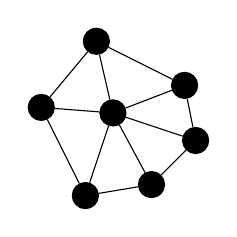
\begin{tikzpicture}[scale=.7,every node/.style={draw,shape=circle,fill=black,minimum size=1pt}]
% vertices
\path (0.5,1.5) node (p0) {}
(0,0) node (p1) {}
(1.2,0.2) node (p2) {}
(2,1) node (p3) {}
(1.8,2) node (p4) {}
(0.2,2.8) node (p5) {}
(-0.8,1.6) node (p6) {};
% edges
\draw (p0) -- (p1)
(p0) -- (p2)
(p0) -- (p3)
(p0) -- (p4)
(p0) -- (p5)
(p0) -- (p6)
(p1) -- (p2)
(p2) -- (p3)
(p3) -- (p4)
(p4) -- (p5)
(p5) -- (p6)
(p6) -- (p1);
\end{tikzpicture}
\label{fig:GeneralSimple}
}
\hfil
\subfloat[]{
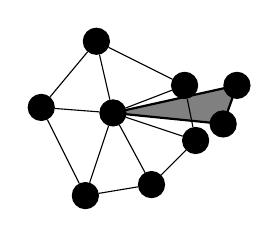
\begin{tikzpicture}[scale=.7,every node/.style={draw,shape=circle,fill=black,minimum size=1pt}]
\draw [fill=gray,thick] (0.5,1.5) -- (2.5,1.3) -- (2.75,2) -- (0.5,1.5);
% vertices
\path (0.5,1.5) node (p0) {}
(0,0) node (p1) {}
(1.2,0.2) node (p2) {}
(2,1) node (p3) {}
(1.8,2) node (p4) {}
(0.2,2.8) node (p5) {}
(-0.8,1.6) node (p6) {}
(2.5,1.3) node (p7) {}
(2.75,2) node (p8) {};
% edges
\draw (p0) -- (p1)
(p0) -- (p2)
(p0) -- (p3)
(p0) -- (p4)
(p0) -- (p5)
(p0) -- (p6)
(p1) -- (p2)
(p2) -- (p3)
(p3) -- (p4)
(p4) -- (p5)
(p5) -- (p6)
(p6) -- (p1);
\end{tikzpicture}
\label{fig:Complex}
}
\hfil
\subfloat[]{
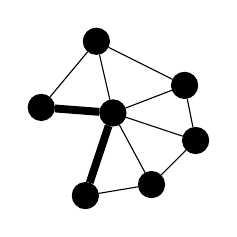
\begin{tikzpicture}[scale=.7,every node/.style={draw,shape=circle,fill=black,minimum size=1pt}]
% vertices
\path (0.5,1.5) node (p0) {}
(0,0) node (p1) {}
(1.2,0.2) node (p2) {}
(2,1) node (p3) {}
(1.8,2) node (p4) {}
(0.2,2.8) node (p5) {}
(-0.8,1.6) node (p6) {};
% edges
\draw (p0) -- (p1)
(p0) -- (p2)
(p0) -- (p3)
(p0) -- (p4)
(p0) -- (p5)
(p0) -- (p6)
(p1) -- (p2)
(p2) -- (p3)
(p3) -- (p4)
(p4) -- (p5)
(p5) -- (p6);
\draw [line width=.1cm] (p1) -- (p0) -- (p6);
\end{tikzpicture}
\label{fig:Boundary}
}
\hfil
\subfloat[]{
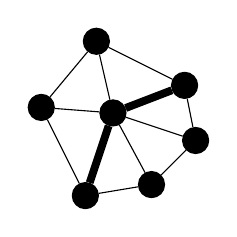
\begin{tikzpicture}[scale=.7,every node/.style={draw,shape=circle,fill=black,minimum size=1pt}]
% vertices
\path (0.5,1.5) node (p0) {}
(0,0) node (p1) {}
(1.2,0.2) node (p2) {}
(2,1) node (p3) {}
(1.8,2) node (p4) {}
(0.2,2.8) node (p5) {}
(-0.8,1.6) node (p6) {};
% edges
\draw (p0) -- (p1)
(p0) -- (p2)
(p0) -- (p3)
(p0) -- (p4)
(p0) -- (p5)
(p0) -- (p6)
(p1) -- (p2)
(p2) -- (p3)
(p3) -- (p4)
(p4) -- (p5)
(p5) -- (p6)
(p6) -- (p1);
\draw [line width=.1cm] (p1) -- (p0) -- (p4);
\end{tikzpicture}
\label{fig:InteriorEdge}
}
\hfil
\subfloat[]{
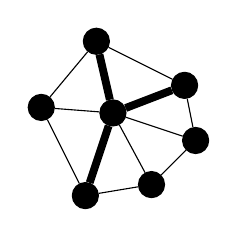
\begin{tikzpicture}[scale=.7,every node/.style={draw,shape=circle,fill=black,minimum size=1pt}]
% vertices
\path (0.5,1.5) node (p0) {}
(0,0) node (p1) {}
(1.2,0.2) node (p2) {}
(2,1) node (p3) {}
(1.8,2) node (p4) {}
(0.2,2.8) node (p5) {}
(-0.8,1.6) node (p6) {};
% edges
\draw (p0) -- (p1)
(p0) -- (p2)
(p0) -- (p3)
(p0) -- (p4)
(p0) -- (p5)
(p0) -- (p6)
(p1) -- (p2)
(p2) -- (p3)
(p3) -- (p4)
(p4) -- (p5)
(p5) -- (p6)
(p6) -- (p1);
\draw [line width=.1cm] (p1) -- (p0) -- (p4);
\draw [line width=.1cm] (p0) -- (p5);
\end{tikzpicture}
\label{fig:Corner}
}
\caption{Five classes of the vertex in the surface. (a) General simple case; (b) Complex case; (c) Boundary case; (d) Interior edge case; (e) Corner case. }%
\label{fig:FiveClasses}
\end{figure}
\begin{figure}[t]
\centering
\subfloat[]{
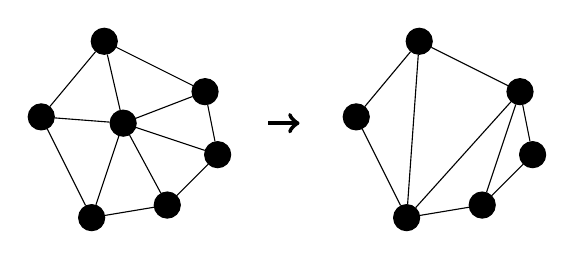
\begin{tikzpicture}[scale=.8,every node/.style={draw,shape=circle,fill=black,minimum size=3pt}]
% vertices
\path (0.5,1.5) node (p0) {}
(0,0) node (p1) {}
(1.2,0.2) node (p2) {}
(2,1) node (p3) {}
(1.8,2) node (p4) {}
(0.2,2.8) node (p5) {}
(-0.8,1.6) node (p6) {};
\path %(5.5,1.5) node (p7) {}
(5,0) node (p8) {}
(6.2,0.2) node (p9) {}
(7,1) node (p10) {}
(6.8,2) node (p11) {}
(5.2,2.8) node (p12) {}
(4.2,1.6) node (p13) {};
% edges
\draw (p0) -- (p1)
(p0) -- (p2)
(p0) -- (p3)
(p0) -- (p4)
(p0) -- (p5)
(p0) -- (p6)
(p1) -- (p2)
(p2) -- (p3)
(p3) -- (p4)
(p4) -- (p5)
(p5) -- (p6)
(p6) -- (p1);
\draw (p8) -- (p9)
(p9) -- (p10)
(p10) -- (p11)
(p11) -- (p12)
(p12) -- (p13)
(p13) -- (p8)
(p8) -- (p12)
(p8) -- (p11)
(p9) -- (p11);
% draw arrow
\draw [->,ultra thick] (2.8,1.5) -- (3.3,1.5);
\end{tikzpicture}
\label{fig:SimpleReduction}
}
\hfil
\subfloat[]{
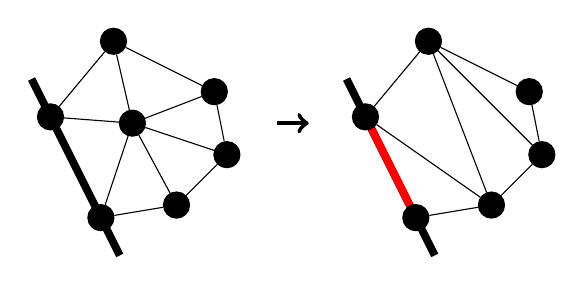
\begin{tikzpicture}[scale=.8,every node/.style={draw,shape=circle,fill=black,minimum size=3pt}]
% vertices
\path (0.5,1.5) node (p0) {}
(0,0) node (p1) {}
(1.2,0.2) node (p2) {}
(2,1) node (p3) {}
(1.8,2) node (p4) {}
(0.2,2.8) node (p5) {}
(-0.8,1.6) node (p6) {};
\path %(5.5,1.5) node (p7) {}
(5,0) node (p8) {}
(6.2,0.2) node (p9) {}
(7,1) node (p10) {}
(6.8,2) node (p11) {}
(5.2,2.8) node (p12) {}
(4.2,1.6) node (p13) {};
% edges
\draw (p0) -- (p1)
(p0) -- (p2)
(p0) -- (p3)
(p0) -- (p4)
(p0) -- (p5)
(p0) -- (p6)
(p1) -- (p2)
(p2) -- (p3)
(p3) -- (p4)
(p4) -- (p5)
(p5) -- (p6);
\draw [line width=0.1cm] (-1.1,2.2) -- (0.3,-0.6);
\draw (p8) -- (p9)
(p9) -- (p10)
(p10) -- (p11)
(p11) -- (p12)
(p12) -- (p13)
(p13) -- (p8)
(p9) -- (p13)
(p9) -- (p12)
(p10) -- (p12);
\draw [line width=0.1cm] (3.9,2.2) -- (5.3,-0.6);
\draw [line width=0.1cm,red] (p8) -- (p13);
% draw arrow
\draw [->,ultra thick] (2.8,1.5) -- (3.3,1.5);
\end{tikzpicture}
\label{fig:BoundaryReduction}
}
\caption{Reduction of polygons before and after eliminating the vertex. (a) General simple vertex case: number of polygons before reduction: $6$, number of polygons after reduction: $4$; (b) Boundary vertex case: number of polygons before reduction: $5$, number of polygons after reduction: $4$. Note that the edge in \emph{red} does not belong to the surface before the computation. }%
\label{fig:Reduction}
\end{figure}

To delete the unimportant vertices, some criteria must be designed and applied to validate the geometry of all potential targets among the model.
First of all, the complex vertices are definitely retained.
Then the rest are well checked to decide whether delete or not.
For the simple vertices that are not located on the boundary or the interior edge, the distance from them to the average plane is the unique principle -- if the distance is less than a certain value, it will be preserved; if not, it will be deleted. %
The vertices on the boundary or the interior edge are checked in the similar way -- if the distance is less than a certain value, it will be retained; otherwise, it will be kicked out. %
The vertices located at corners are usually preserved to maintain the approximation of the original geometry or left the ``noises" introduced in the modeling phase to be depressed by using appropriate method. %

Once upon the deletion of the vertex and its associated edges, one (in simple case) or two holes (in boundary or interior edge case) are left for patching thus maintaining the surface. In achieving the new patches for these holes, new triangulation at the location is created, which is done before the actual deletion mentioned before.

Comparing the number of triangles before and after this process, two triangles are reduced for the cases of general simple vertices, interior edge vertices, and some corner vertices; whilst one for the cases of vertices located at the boundaries (see Fig. \ref{fig:Reduction}). %

%# -*- coding:utf-8 -*-
\section{Experiments and Results}
\label{sec6_2}

\subsection{Data and Experimental Setup}

The vasculature surface models were generated by applying the approaches proposed in \cite{Yang2014ICRA} from the original CTA images.
The resolution of the original data was $0.4 \times 0.4 \times 0.6 \text{mm}^3$.
For the sake of simplicity, only a segment of the abdominal aorta is depicted in this paper to demonstrate the effectiveness of our approach (see Fig. \ref{fig:VOI}).
The approach can be ported in order to process the model surfaces of the whole vasculature related to the surgical procedure to be simulated.

All of our experimental programs ran on a desktop machine equipped with Intel's 2.83GHz Core 2 Quad CPU and 4GB RAM.

\begin{figure}[t]
\centering
\includegraphics[height=2.0in]{Figures/chap06/original.png}
\caption{VOI-extracted surface model consisting of $74307$ polygons.}
\label{fig:VOI}
\end{figure}

\subsection{Validating Connectivity Between Vertices}

First of all, the polygonal elements in the patient-specific surface model of the human vessels need to be checked such that the connectivity between any pair of vertices are validated. %
After doing this, the integration of the model surface is guaranteed that the excessive polygons are kicked off.
Table \ref{tbl:Connectivity} shows that the total number of the polygonal surfaces were not changed, which implies that the given model (i.e., the local one) was already the largest-connected region in the model before the validation process. %

\subsection{Smoothing Model Surface}

Since the unavoidable noises introduced in the phase of image acquisition and processing, uneven surfaces may be found in the surface rendered based on the imagery.
The mess of artifacts and crusts may induce the problems in the smoothness of the delivery of the virtual surgical tools, e.g., guidewires, catheters, etc.
To avoid this situation, a thorough smoothing process is needed on the inner surface of the model, which is equivalent to the smoothing on the model surface per se.
\begin{table}[t]
\renewcommand{\arraystretch}{1.3}
\caption{Numbers of polygons before and after connectivity validation}
\label{tbl:Connectivity}
\centering
\begin{tabular}
{@{}l||r@{}}
%{@{}llrr@{}}
%\toprule
\hline
~                       & No. of polygons \\
\hline\hline
Before validation       & $74,307$  \\
After validation        & $74,307$  \\
\hline
\end{tabular}
\end{table}

The algorithm utilized in this processing task is implemented based on the low-pass filtering principles, with two parameters to be tuned in control of the smoothing effect on the objects. %
One of the parameters regulates the number of iterations the algorithm should take.
It is equivalent to the order of the polynomial that approximating the windowed sinc function given in (\ref{eqn:Approximation}).
The other parameter is used to configure the bandwidth of this so-called low-pass filter.

In this work, several parameter sets were given with the aim of searching for the one that can generate the most acceptable results.
The numbers of iterations of the smoothing were chosen to be $30$, $60$, and $100$ in the two cases, where the bandwidths were $0.1$, and $0.01$.

Judging from the resultant models in Fig. \ref{fig:Smooth}, the ones on the top row (see Figures \ref{fig:Smooth30-1}, \ref{fig:Smooth60-1}, and \ref{fig:Smooth100-1}) smoothed with the bandwidth $0.1$ are still fairly rough compared to the input, while the ones on the bottom row (see Figures \ref{fig:Smooth30-01}, \ref{fig:Smooth60-01}, and \ref{fig:Smooth100-01}) with the bandwidth $0.01$ are much better. %
With the increase of the number of iterations, the smoothing effect became more apparent, compared with the column of results from the one on its left.
At this stage of processing, we chose the parameter set which was used to generated the results depicted in Fig. \ref{fig:Smooth100-01} ($\text{no. of iterations} = 100$, $\text{pass band} = 0.01$). %
\begin{figure}[t]
\centering
\subfloat[]{\includegraphics[height=2.0in]{Figures/chap06/smooth_30_1.png}%
\label{fig:Smooth30-1}}
\hfil
\subfloat[]{\includegraphics[height=2.0in]{Figures/chap06/smooth_60_1.png}%
\label{fig:Smooth60-1}}
\hfil
\subfloat[]{\includegraphics[height=2.0in]{Figures/chap06/smooth_100_1.png}%
\label{fig:Smooth100-1}}
\hfil
\subfloat[]{\includegraphics[height=2.0in]{Figures/chap06/smooth_30_01.png}%
\label{fig:Smooth30-01}}
\hfil
\subfloat[]{\includegraphics[height=2.0in]{Figures/chap06/smooth_60_01.png}%
\label{fig:Smooth60-01}}
\hfil
\subfloat[]{\includegraphics[height=2.0in]{Figures/chap06/smooth_100_01.png}%
\label{fig:Smooth100-01}}
\caption{Smoothing effects by applying different parameters: top row illustrate the results with $\text{pass band} = 0.1$, and the numbers of iterations are: $30$, $60$, and $100$, respectively; bottom row illustrate the results with $\text{pass band} = 0.01$, and the numbers of iterations are: $30$, $60$, and $100$, respectively.}%
\label{fig:Smooth}
\end{figure}

\subsection{Elimination of Component Polygons}

The elimination of polygon elements of the model surface was conducted after the smoothing computation terminated demonstrated in the last section.

For the input surface model, over $74$k polygons were required to model the vessel segment by using Marching Cubes method \cite{Lorensen1987MC}.
One can imagine that the overall number of the polygons needed to model the whole aorta and the trees of the coronary arteries.
Rendering the large amount of data will surely exhaust the most memory on any machine with typical hardware configuration, thus no sufficient space could be spared for the interaction and other computation.
To facilitate this situation, we adopted the decimation algorithm introduced in Section \ref{subsec:decimation} with multiple sets of parameters in a series of experiments. %

In this work, the termination conditions of the adopted algorithm were set to $10\%$, $50\%$, $75\%$, $90\%$, and $99\%$, respectively.
By termination condition, which is equivalent to the reduction rate, we mean that the rate of the total number of the polygonal elements deleted with respect to the total number of the polygonal elements in the input model surface. %
This can be written as follows
\begin{equation}
\label{eqn:ReductionRate}
\text{Reduction Rate (\%)} = \frac{\text{No. of \emph{deleted} Polygons}}{\text{No. of Input Polygons}}.
\end{equation}

Table \ref{tbl:Decimate} illustrates the effects of the decimation algorithm.
Figure \ref{fig:Decimate} depicts the visualization results of the decimation with typical parameters.
Observing the results, visualization in Figures \ref{fig:Decimate90} and \ref{fig:Decimate99} contain acceptable amounts of polygons.
However, the visualization in fig. \ref{fig:Decimate99} unveiled obvious alterations in its geometry.

\subsection{Discussions}

All the programs ran in the experiments were written in C++.
Some of the functioning modules were implemented based on the Visualization Toolkit (VTK) \cite{Schroeder2000VTK}, an open source effort containing various of computation facilities implementing algorithms from both the general and special fields of computer graphics. %

In validating the connectivity of the adjacent points among the surface model, the algorithm was configured to extract the largest-connected areas in this work.
To depress the effects from the noisy meshes introduced by image processing, a surface smoothing algorithm was employed to remove these meshes by slightly altering the locations of the vertices of the meshes. %
In smoothing the surface, two distinct parameters were the key switches for the algorithm, among which the width of the pass band of the low-pass filter and the number of the iterations to be performed were determined. %
Between the number of iterations and the smoothing effects on the surface, a positive correlation was demonstrated that the larger the number, the smoother the result.
On the other hand, the width of the pass band and the smoothing effects implied a negative correlation that the narrower the pass band, the smoother the result.
%One thing to be noted is that the loss of certain details occurred on all the resultant surface models.
\begin{table}[t]
\renewcommand{\arraystretch}{1.3}
\caption{Reduction rates and quantities of polygons in the model surface after decimation}
\label{tbl:Decimate}
\centering
\begin{tabular}{c||r r r r r}
\hline
%\bfseries      & \bfseries Quantity of polygonal surfaces \\
Reduction Rate ($\%$)  &    $10$ &    $50$ &    $75$ &   $90$ &  $99$ \\
\hline\hline
No. of Polygons & $66875$ & $37153$ & $18576$ & $7430$ & $743$ \\
\hline
\end{tabular}
\end{table}
\begin{figure}[t]
\centering
\subfloat[]{\includegraphics[height=2.0in]{Figures/chap06/smooth_100_01_d10.png}%
\label{fig:Decimate10}}
\hfil
\subfloat[]{\includegraphics[height=2.0in]{Figures/chap06/smooth_100_01_d90.png}%
\label{fig:Decimate90}}
\hfil
\subfloat[]{\includegraphics[height=2.0in]{Figures/chap06/smooth_100_01_d99.png}%
\label{fig:Decimate99}}
\hfil
\subfloat[]{\includegraphics[height=2.0in]{Figures/chap06/smooth_100_01_d10_w.png}%
\label{fig:Decimate10-w}}
\hfil
\subfloat[]{\includegraphics[height=2.0in]{Figures/chap06/smooth_100_01_d90_w.png}%
\label{fig:Decimate90-w}}
\hfil
\subfloat[]{\includegraphics[height=2.0in]{Figures/chap06/smooth_100_01_d99_w.png}%
\label{fig:Decimate99-w}}
\caption{Decimation effects by applying different parameters: top row illustrate the results with reduction rates of $10\%$, $90\%$, and $99\%$, respectively; bottom row illustrate the wire frame representation of the corresponding results depicted above.}%
\label{fig:Decimate}
\end{figure}

In decimating the polygons, the problem is two-folded: on the one hand, the higher rate of reduction is preferred for the following interaction system; on the other hand, however, the over high rate of reduction may lead to heavy tortures on the model surface thus the geometry is doomed to be destroyed. %
This should be taken into consideration when selecting the reduction rate for the decimator algorithm.
In this work, we have tested series of cases with different rates and successfully determined the one that was acceptable in eliminating the excessive polygons.
The output of the decimation process are the progressive meshes \cite{Hoppe1996}.
Besides the aforementioned decimation on the input meshes, the resultant meshes had well preserved the geometry of the model, as well as its global appearance (normals, color values, etc.). %

%# -*- coding:utf-8 -*-

\section{Conclusions and Future Work}
%The conclusion goes here.

In the context of simulating the intravascular surgical procedure, the interactive performance between the virtual surgical tools (i.e., catheters or guidewires) and the vasculature is one of the most important benchmarks. %
The amount of the data used to model the surface of the related vasculature is one of the main factors.
In this paper, we developed an approach in order to address this problem.
The basic idea is to eliminate the polygon components consisting the model surface without destroying the geometry of the vasculature.
The data used in the experiments were the patient-specific vessel model generated by series of image processing on the original CT dataset in our previous work.

First of all, the connectivity between the adjacent vertices was validated and the unconnected vertices were removed.
Then the noisy surfaces introduced from the image acquisition and processing were smoothed with the least effects on the model's geometry.
Finally the decimation pass was introduced to reduce the number of the polygon components at the desired reduction rate.
In reducing the polygonal elements, not only did we consider the number of the polygons that had been removed, but also the visualization of the resultant models.
Experimental results illustrated the effectiveness of our approach in reducing the quantities of the polygonal elements in the surface model.

Our future work will be the visualization of other human organs (e.g., heart, skeletons, etc.) appeared in the field of real surgeries on the one hand, and the physical modeling of the virtual human organs on the other. %


%# -*- coding:utf-8 -*-
\chapter{基于CTA的心脏分割与可视化}
\label{chap7}

%# -*- coding:utf-8 -*-
本章敘述內容:
\begin{enumerate}
  \item 引言
  \item 状态机的原理
  \item 介入式冠脉导管术的流程
  \item 介入导管术流程的状态机化
  \item 实际验证
  \item 本章小结
\end{enumerate}
%# -*- coding:utf-8 -*-
\section{引言}
\label{sec7-1} 

Coronary heart diseases (CHDs), ranking among the top ten list of the non-accidental causes of deaths, are the malformations of the coronary arteries through which the nutrition supply is transported to the heart muscle \cite{WHO2013}. %
The diseases had spread in both developed and developing countries all over the world.
The main reasons that cause CHDs include cigarette smoking, lack of exercises, depressed mood, pressures from work and life, unhealthy diet, and obesity \cite{Go2013}.

As the key procedure in revascularization, percutaneous coronary intervention (PCI) are conducted in the catheterization laboratories of different continents to save hundreds of lives. %
Small incisions and short period of operation make the procedure incur traumas to the patients as slight as possible; whilst make the learning of it more difficult for the novice in the labs. %

In learning this technique, one has to fully understand the vascular anatomy, to choose the proper catheters or guidewires at the right time, and to overcome the difficulties of the eye-hand coordination \cite{Li2012CUHK}. %
The traditional ways of training rely on human cadavers, living animals, physical simulators made of non-biological materials.
However, the expenditure on keeping the cadavers and feeding the animals are extremely high, while the physical simulators can only provide poor intuition for the trainees.
The situation went worse after the invention and application of the surgical robotic systems, i.e., the high-end machinery also require the users to receive proper and sufficient training before the real robot-assisted operation. %
To streamline this process, several computer-aided simulators have been designed and already demonstrated their advantages \cite{Liss2012}.

The ultimate goal is to design and implement a computer-enhanced surgical simulation system for the training of the intravascular surgical robot built in our lab \cite{Ji2011EMBC}.
The whole work is organized into two integral parts: one is the reconstruction of the human anatomy, and the other is the simulation of the surgical tools.
In this paper, we proposed an approach to segment and visualize the heart in the original CT information, aiming to provide sufficient intuition to the users when interacting with the computer-aided surgical simulation system under construction. %
The main idea in this paper is based on our previous work in segmenting the blood vessels \cite{Yang2014ICRA}.
The resultant heart model, enveloped by the coronary arteries \cite{Yang2013ROBIO}, enables the users judging the directions and spatial relationship of the complicated branches of the vasculature more conveniently. %

The remainder of this paper is organized as follows.
Section II outlines the work flow and details the techniques used in this work.
Section III describes the experiments with a brief discussion.
The final section concludes the whole work and outlooks the future.
%# -*- coding:utf-8 -*-
\section{方法}
\label{sec7-2} 
%# -*- coding:utf-8 -*-
\section{实验与结果}
\label{sec7-3}

\subsection{Original Data and Experimental Setup}

Considering our aim and the requirements on the computation resources, the volume containing the whole heart was extracted from the original one that include the whole body trunk of an anonymous patient. %
The dataset, in resolution of $0.4\text{mm} \times 0.4\text{mm} \times 0.6\text{mm}$, was acquired on a 128-slice CT modality (Siemens SOMATOM Definition Flash).
\begin{figure}[t]
\centering
\includegraphics[height=2.0in]{Figures/chap07/original.pdf}
\caption{The anterior view of the original volume contains the whole heart extracted from the raw CT information.}
\label{fig:Original}
\end{figure}
\begin{figure}[t]
\centering
\includegraphics[height=2.0in]{Figures/chap07/binary_threshold.pdf}
\caption{Volume after binary threshold processing. Note that the pericardium, and most of the blood vessels are excluded.}%
\label{fig:BinaryThreshold}
\end{figure}

Numbers of experimental trials were carried out on the image dataset, applying distinct sets of parameters for the evaluation of the approach.
%In our case, the CTA series in DICOM format had been converted to the form of XML first.
%Then the converted data was fed into the feature image production branch and input level sets generation branch.
%The resulting data from the two branches were sent to geodesic active contours module in order to generate the final results.
%Finally, the marching cubes method is used to visualize the segmented data.
The experiments were executed on a desktop machine armed with Intel's 2.83GHz Core 2 Quad CPU and 4GB RAM.

\subsection{Preprocessing}

As mentioned in Sec. \ref{sec:overview}, series of preprocessing were conducted before the evolution of the ``snakes":
(i) the image smoothing preserving the edges;
(ii) the exclusion of the uninterested image details;
(iii) the calculation of the image gradient magnitude;
(iv) the generation of the initial contours.

As the first step, an algorithm based on MCDE given by (\ref{eqn:MCDE}) was utilized to smooth the input images.
By applying this numerical method, the edges in the images were well protected from the smoothing effect.

Then the binary thresholding was applied to archived the goal -- excluding most uninteresting contents, i.e., only the contents of interest were left after this step.
To achieve this goal, the properly chosen threshold pairs were decided based on the analysis of the histogram of the smoothing images.
Figure \ref{fig:BinaryThreshold} depicted the results of the binary thresholding step.

After thresholding the images, the rest two steps (the calculation of the edge potential and the initial contours) were performed simultaneously.

In calculating the edge potential of the images, the work was divided into two consecutive steps:
Firstly, the gradient magnitude of the images were calculated by solving (\ref{eqn:Gaussian}).
Secondly, the results of the previous step were converted into the appearance that the edges are dark while the rest of the images are bright.
In converting the gradient images, the selection of the parameters $m$ and $n$ in (\ref{eqn:Sigmoid}) were essential.
Their values depended the two extreme intensities of the pixels in the gradient images.
In the experiments, the guideline of the selection was: $m < 0$, and $n > 0$, where $n > |m|$.
The resultant images demonstrated the edges of the objects in zero intensity while the inside/outside areas in the maximum intensity (i.e., $255$).
%\begin{figure*}[t]
%\centering
%\subfloat[]{\includegraphics[height=2.5in]{../Figures/heart.eps}
%\label{fig:Heart}}
%\hfil
%\subfloat[]{\includegraphics[height=2.5in]{../Figures/heart_with_ca.eps}
%\label{fig:Overlay}}
%\caption{The resultant models of this paper. (a) the three-dimensional model of the heart; (b) the overlayed three-dimensional models of the heart and the coronary arteries acquired in the previous work \cite{Yang2013ROBIO} are rendered in the same scene.}%
%\label{fig:HeartModel}
%\end{figure*}

Meanwhile, the evolution, driven by the fast marching algorithm \cite{Sethian1999}, started with the aim of generating the initial contours for the geodesic ``snakes" computation.
The results provided the geodesic computation the \emph{time-crossing} map so that the ``snakes" can evolve according to the computed time-of-arrival.
In this step, the only human intervention was the selection of the input seeding points, from which the computation would begin.
The location of the seeds should be located interior of the targets, and the sign of the speed function $F$ in (\ref{eqn:Eikonal}) should be positive to ensure outwards propagation of the contours. %

\subsection{Level Set Computation of Geodesic ``Snakes"}

The evolution of the geodesic ``snakes" started from the seeding points fed in previous step for the generation of the initial contours.
The ``snakes" utilized the resultant initial contours as the map in which all the pixels were marked with the time when the fronts ever crossed them.
On the other hand, that edge potential maps depicted the general geometric feature of the images, in which the magnitudes of the gradients were calculated and represented to show the ``valleys" and the ``plains" in the images. %

In order to speed up the calculation, sufficient ``attraction" in (\ref{eqn:GeodesicDriver}) was required.
Besides, the disturbance of the false edges during the evolution can be avoided due to larger attraction.
In this work, the original contours were located inside of the targets, meaning that they evolved ``outwards" towards the edges.
During the computation, the speed of the propagation was fast on the ``plains" (i.e., the inner areas of the targets), and was pretty slow when falling into the ``valleys" (i.e., the edges of the targets). %
To terminate the computation in time, the numbers of the iterations was set to $500$ in the experiments.
\begin{figure}[t]
\centering
\includegraphics[height=2.4in]{Figures/chap07/heart.pdf}
\caption{The anterior view of the three-dimensional surface model of the heart.}
\label{fig:Heart}
\end{figure}

%# -*- coding:utf-8 -*-
\section{讨论}
\label{sec7-4} 

%# -*- coding:utf-8 -*-
\chapter{虚拟手术中主要医学操作的可视化效果}
\label{chap8}

%# -*- coding:utf-8 -*-
如果上述基本要求能够在较短时间内顺利实现,则把工作的重心转移的实现系统的高级要求上来。
系统的高级特性包括:血管模型应具备与真实血管相近的弹性和形变特性;所重建的心脏区域
(指冠状动脉和心房与心室)可以虚拟心脏的搏动过程;实现虚拟造影剂,该特性在触觉操作机
构的激发下呈现,应当具有与真实手术过程中,医生通过导管向冠状动脉中注入造影剂时的视觉
效果应当一致;实现虚拟支架-气囊,使其能够像真实情况一样--在气囊内部被气体填充的过程
中,支架的结构发生变化、内径逐渐增大;操作过程记录;训练难度分级与训练评价等。

%# -*- coding:utf-8 -*-
\section{球囊模型}
\label{sec8-1}
%# -*- coding:utf-8 -*-
\section{器官运动模型}
\label{sec8-2}
%# -*- coding:utf-8 -*-
\section{造影剂注射仿真}
\label{sec8-3}
%# -*- coding:utf-8 -*-
\section{X光可视效果与视角协调}
\label{sec8-4} 
%# -*- coding:utf-8 -*-
\section{本章小结}
\label{sec8-5} 
%# -*- coding:utf-8 -*-
\chapter{虚拟手术的过程模型}
\label{chap9}

%# -*- coding:utf-8 -*-
本章敘述內容:
\begin{enumerate}
  \item 引言
  \item 状态机的原理
  \item 介入式冠脉导管术的流程
  \item 介入导管术流程的状态机化
  \item 实际验证
  \item 本章小结
\end{enumerate} 
%# -*- coding:utf-8 -*-
\section{引言}
\label{sec9_1}
%# -*- coding:utf-8 -*-
\section{状态机的原理}
\label{sec9_2}
%# -*- coding:utf-8 -*-
\section{介入式冠脉导管术的流程}
\label{sec9_3}
%# -*- coding:utf-8 -*-
\section{介入导管术流程的状态机化}
\label{sec9_4}
%# -*- coding:utf-8 -*-
\section{实际验证}
\label{sec9_5} 
%# -*- coding:utf-8 -*-
\section{本章小结} 
\label{sec9_6} 

%# -*- coding:utf-8 -*-
\chapter{总结与展望}
\label{chap10}

%# -*- coding:utf-8 -*-
如果上述基本要求能够在较短时间内顺利实现,则把工作的重心转移的实现系统的高级要求上来。
系统的高级特性包括:血管模型应具备与真实血管相近的弹性和形变特性;所重建的心脏区域
(指冠状动脉和心房与心室)可以虚拟心脏的搏动过程;实现虚拟造影剂,该特性在触觉操作机
构的激发下呈现,应当具有与真实手术过程中,医生通过导管向冠状动脉中注入造影剂时的视觉
效果应当一致;实现虚拟支架-气囊,使其能够像真实情况一样--在气囊内部被气体填充的过程
中,支架的结构发生变化、内径逐渐增大;操作过程记录;训练难度分级与训练评价等。
%# -*- coding:utf-8 -*-
\section{总结}
\label{sec10-1}
%# -*- coding:utf-8 -*-
\section{展望}
\label{sec10-2}




% 附录
\begin{appendix}
\renewcommand{\chaptername}{附录 \Alph{chapter}}
%# -*- coding:utf-8 -*-
\chapter{软件系统的整合}
\label{chap1a}

本章叙述内容:
\begin{enumerate}
  \item 引言
  \item 软件系统的设计
  \item 相关的软件库
  \item 工程注记
  \item 本章小结
\end{enumerate}

\section{引言}

\section{软件系统的设计}

\section{相关的软件库}

\section{工程注记}

\section{本章小结} 
%# -*- coding:utf-8 -*-
\chapter{软件系统的整合}
\label{chap1a}

本章叙述内容:
\begin{enumerate}
  \item 引言
  \item 软件系统的设计
  \item 相关的软件库
  \item 工程注记
  \item 本章小结
\end{enumerate}

\section{引言}

\section{软件系统的设计}

\section{相关的软件库}

\section{工程注记}

\section{本章小结} 
\end{appendix}
\backmatter %结束章节自动编号

%参考文献
\cleardoublepage
\phantomsection
\bibliographystyle{thubib}
%\bibliographystyle{unsrt}
\addcontentsline{toc}{chapter}{参考文献}
\addtolength{\bibsep}{-4.5pt} % 缩小参考文献间的垂直间距
\bibliography{Reference/myreference_UTF8}

%\frontmatter
%攻读博士学位期间的研究成果
%# -*- coding:utf-8 -*- 
%=========================================================================%
%   LaTeX File for phd thesis of Institute of Automation, CAS
%-------------------------------------------------------------------------%
%   Revised by J. G. Lou (jglou@nlpr.ia.ac.cn)
%-------------------------------------------------------------------------%
%%%%%%%%%%%%%%%%%%%%%%%%%%%%%%%%%%%%%%%%%%%%%%%%%%%%%%%%%%%%%%%%%%%%%%%%%

\chapter*{攻读博士期间发表的论文\markboth{攻读博士学位期间发表的论文}{攻读博士学位期间发表的论文}}
\addcontentsline{toc}{chapter}{攻读博士学位期间发表的论文}
\begin{enumerate}
   \item[1.] \textbf{Fan Yang}, Zeng-Guang Hou, Shao-Hua Mi, Gui-Bin Bian and Xiao-Liang Xie, "3D Modeling of Coronary Arteries Based on Tubular-Enhanced CURVES Segmented Regions for Robotic Surgical Simulation", 2013 International Conference (IEEE-ROBIO 2013) on Robotics and Biomimetics, 12th December 2013.
%   \item[2.] \textbf{楼建光},柳崎峰,胡卫明,谭铁牛, "交通视觉监控中的摄像机参数求解", 计算机学报, 第25卷, 第11册, 2002年11月.
%   \item[3.] \textbf{Jianguang Lou}, Qifeng Liu, Tieniu Tan and Weiming Hu, "Semantic interpretation of object activities in a surveillance system", IEEE International Conference on Pattern Recognition, Canada, 2002 (\textbf{oral presentation}).
%   \item[4.] \textbf{Jianguang Lou}, Hao Yang, Weiming Hu, Tieniu Tan, "Visual Vehicle Tracking Using An Improved EKF", the 5th Asia Conference on Computer Vision, Australia, 2002 (\textbf{oral presentation}).
%   \item[5.] \textbf{Jianguang Lou}, Hao Yang, Weiming Hu, Tieniu Tan, "An Illumination Invariant Change Detection Algorithm", the 5th Asia Conference on Computer Vision, Australia, 2002 (\textbf{oral presentation}).
%   \item[6.] Hao Yang, \textbf{Jianguang Lou}, Hongzan Sun, Weiming Hu and Tieniu Tan, "Efficient and robust vehicle localization", Proceeding of IEEE International Conference on Image Processing, Vol.2, pp. 355-358, Greece, 2001.
%   \item[7.] Qifeng Liu, \textbf{Jianguang Lou}, Weiming Hu, Tieniu Tan, "Comparison of model-based pose evaluation algorithm in traffic scenes", the 2nd International Conference on Image and Graphics, Hefei, 2002.
%   \item[8.] 柳崎峰,\textbf{楼建光},"智能视觉监控技术",科学新闻,第23期,pp. 35-36, 2002年12月.
\end{enumerate}



% 致谢
%# -*- coding:utf-8 -*- 
%=========================================================================%
%   LaTeX File for phd thesis of Institute of Automation, CAS
%-------------------------------------------------------------------------%
%   Revised by J. G. Lou (jglou@nlpr.ia.ac.cn)
%-------------------------------------------------------------------------%
%%%%%%%%%%%%%%%%%%%%%%%%%%%%%%%%%%%%%%%%%%%%%%%%%%%%%%%%%%%%%%%%%%%%%%%%%

\chapter*{致\ 谢\markboth{致\ 谢}{致\ 谢}}
\addcontentsline{toc}{chapter}{致谢}



值此学位论文完成之际,我要向我的导师侯增广研究员表示最衷心感谢。老师渊博的学识,
对学术发展的敏锐眼光,对科研事业的执着追求和对工作的热忱,以及对我们研究生的关
心和爱护,都深深地鼓舞和影响了我。所有这些,都令学生受益终生!

感谢复杂系统管理与控制国家重点实验室机器人研究组的各位老师为我们营造的这样一个
良好的学习环境。感谢同组已毕业的同学吉程博士和徐飞硕士,与他们的讨论激发了我的
创意和兴趣;感谢同组同届的同学米韶华和陈翼雄,这共同攻读博士学位的“苦难岁月”
让我们成为了战友;感谢同组的其他同学对我的帮助和支持。同机器人研究组的导师和同
学一起学习和工作的时光,将是我个人学习生涯中最难以忘怀的。

感谢上海市胸科医院的方唯一教授和曲新凯博士,感谢他们在百忙中抽出宝贵的时间为我
们耐心地讲解和演示经皮介入冠状动脉导管术,热心回复我们在工作中遇到的医学方面的
问题,并为我们提供了宝贵的医学资料。

感谢开源软件社区的每一位黑客,感谢他们在智慧上的无私分享。如果没有这些设计优雅、
性能优异的专业级别的开源软件工具,那么我们的研究工作很可能无法在这短短几年中完
成。

感谢中国科学院自动化研究所研究生部的各位工作人员为我在研究所学习和工作期间提供
的咨询和帮助。

最深的感谢送给我的父母,感谢他们孜孜不倦的教诲和无限的宽容与鼓励。感谢我的妹妹,
家庭的开心果,感谢与她共同成长成人的岁月,感谢她带给我们的每一次开怀大笑。最后,
我要感谢我的妻子,感谢她给我无尽的爱和支持。
\\
\\
\\
\\
\hspace*{10.8cm}2013年10月


\clearpage
\end{CJK*}
\end{document}
%%%%%%%%%%%%%%%%%% End of the file  %%%%%%%%%%%%%%%%%%%%%%%%
